\documentclass[12pt,a4paper]{scrartcl} 

%Deutsch:
	\usepackage[ngerman]{babel} %Deutsches Datumformat, Umlaute m\"oglich,...
	\usepackage[utf8]{inputenc}
	\usepackage[T1]{fontenc} 
	
%Quellenverzeichnis:
	\usepackage[maxcitenames=2,autocite=footnote,uniquename=full,uniquelist=true,backend=biber]{biblatex} %style=authoryear-icomp
	\usepackage{csquotes} %Hilfspaket für Biblatex
	\bibliography{bib_database.bib} %Datei mit bibliographischen Daten
	\DefineBibliographyStrings{ngerman}{andothers={et\ al\adddot}} % "u.a." zu "et al."
	\DefineBibliographyStrings{ngerman}{and={\&}} % "und" zu "&"

%Mathematik:
	\usepackage{dsfont} %Symbole
	\usepackage{amsmath} %Umgebung
	\usepackage{amssymb} %Symbole
	\usepackage{bbm} %doppelstreifen bei buchstaben (zb symbol für ganze zahlen \mathbbm{Z})
	
%Grafiken:
	\usepackage{graphics}
	\usepackage{graphicx}
	\usepackage{picinpar} %bilder so einfügen, dass text um bilder weiterläuft
	\usepackage{float} %\begin{figure}[H] => Grafik wird HIER eingefügt!

%Euro-Zeichen:
	\usepackage{eurosym}

%Pseudo Code:
	\usepackage{algorithmic}
	\usepackage{algorithm}
	\renewcommand{\algorithmicrequire}{\textbf{Eingabe:}}
	\renewcommand{\algorithmicensure}{\textbf{Ausgabe:}}

%Verzeichnis-struktur darstellen:
	\usepackage{dirtree}

%Tabellen:
	\usepackage{multirow}
	
%Quellcode:
	%\usepackage[numbered,framed]{mcode} %Quellcode darstellen
	
%Englisch:
	%\usepackage[ngerman,english]{babel} %automatisch erzeugte Überschriften etc. auf englisch
	
\DeclareMathOperator*{\argmin}{arg\,min} % Importiere die Einstellungen aus der Präambel

% hier beginnt der eigentliche Inhalt
\begin{document}

% Deckblatt
\begin{titlepage}
	\rmfamily
	\begin{center}
		% Logo
		%\includegraphics[width=0.15\textwidth]{./logo}\\[1cm]
	
		\textsc{\LARGE Statistisches Consulting}\\[1.5cm]

		\textsc{
			\large{	Master Studiengang Statistik\\[0.25cm]
							Institut für Statistik\\[0.25cm]
							Ludwig-Maximilians-Universität München}}\\[0.25cm]
						
		% Title
		\newcommand{\HRule}{\rule{\linewidth}{0.5mm}}
		\HRule \\[0.4cm]
		{\huge \bfseries Online-Marketing der Interhyp AG\\[0.5cm]Analyse von Tracking-Daten}\\[0.4cm]
		\HRule \\[1.5cm]
		
		% Autoren
		\textbf{Daniel Fuckner} d.fuckner@gmx.de\\
		\textbf{Markus Vogler} markus@vogler-lindau.de\\[1.5cm]
	
		% Betreuer und Projektpartner
		\begin{minipage}{0.4\textwidth}
			\begin{flushleft}
				Projektpartner:\\
				\textbf{Nicola Gries} (Interhyp AG)
			\end{flushleft}
		\end{minipage}
		\hfill
		\begin{minipage}{0.4\textwidth}
			\begin{flushright}
				Betreuer:\\
				\textbf{Dr. Fabian Scheipl}
			\end{flushright}
		\end{minipage}
		
		\vfill

		% Datum
		{\large München, 26.08.2014}
		
	\end{center}
\end{titlepage}

%\thispagestyle{plain}
\pagenumbering{roman} %römische Seitennummerierung

%Abstract
\begin{abstract}
\noindent\subsubsection*{Abstract}
Die Interhyp AG ist Vermittler für private Baufinanzierungen. Das primäre Ziel des Marketing der Interhyp AG ist die Kundenakquise. Da etwa 80\% aller Kundenanträge online abgeschickt werden, liegt der Fokus auf dem Online-Marketing, das über verschiedene Kampagnen verfügt. Beispiele sind Kooperationen mit anderen Unternehmen, bezahlte Anzeigen bei Suchmaschinen oder Bannerschaltungen.\\
Die Refined Labs GmbH ist verantwortlich für das Online-Tracking der Werbekampagnen der Interhyp AG. Durch Online-Tracking werden die Werbekontakte eines potentiellen Kunden zu einem sogenannten Funnel zusammengefasst. Am Ende eines jeden Funnels steht das Ausfüllen eines Onlineantrages oder der Abbruch. Man spricht von konvertierten beziehungsweise nicht-konvertierten Funnels.\\
In dieser Arbeit werden die Tracking-Daten zunächst anhand deskriptiver Analysen vorgestellt. Außerdem werden Methodik und Ergebnisse eines zeitdiskreten Survival-Modells und eines Sequential Pattern Mining-Algorithmus beschrieben. Mit Hilfe des zeitdiskreten Survival-Modells, das mit Stochastic Gradient Boosting geschätzt wurde, konnten Zusammenhänge zwischen den erklärenden Variablen und der Wahrscheinlichkeit für eine Konvertierung gefunden werden. Häufige Abfolgen von Kampagnen in den konvertierten und nicht-konvertierten Funnels wurden mit dem Sequential Pattern Mining-Algorithmus entdeckt. Zudem wurden die Funnels in Form eines Netzwerkes visualisiert. Die Daten für dieses Netzwerk und ein Programm, dass die interaktive Betrachtung ermöglicht, ist im elektronischen Anhang enthalten.
\end{abstract}

%Inhaltsverzeichnis
\newpage
\tableofcontents

\newpage
\pagenumbering{arabic} %ab hier wieder normale Seitennummerierung

% Hier beginnt der eigentliche Text
\section{Einleitung} 

\begin{frame}\frametitle{Einleitung} 
	\begin{itemize}
		\item Interhyp AG ist Vermittler für private Baufinanzierungen
		\item Primäres Ziel des Marketing ist die Kundenakquise
		\item Etwa $80 \%$ aller Kundenanträge werden online abgeschickt
		\item Online-Marketing verfügt über verschiedene Kanäle
		\item Refined Labs GmbH ist verantwortlich für das Online-Tracking der Werbekampagnen der Interhyp AG
	\end{itemize}
\end{frame}

\begin{frame}\frametitle{Entstehung eines Funnels (Quelle: Interhyp AG)}
	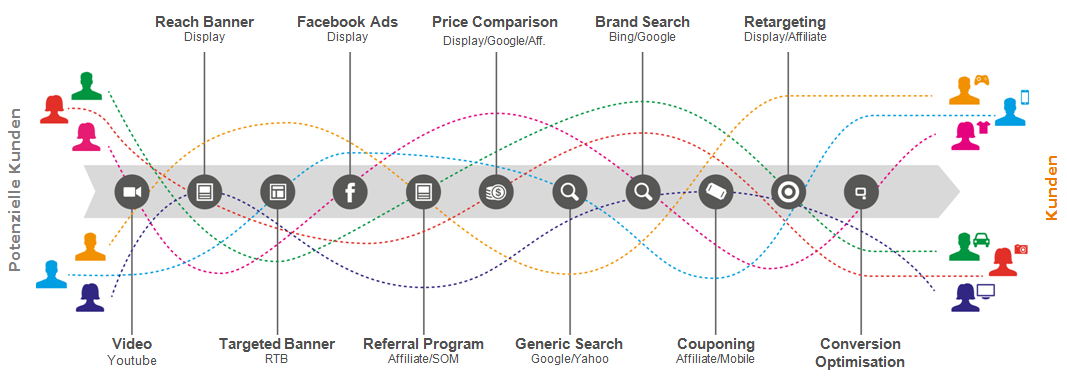
\includegraphics[scale=0.38]{customerJourney.png}\\
	\centering Unterschiede zwischen konvertierten und nicht-konvertierten Funnels?
\end{frame} % Importiere die Einleitung
\section{Datenlage}\label{datenlage}

Die Daten wurden von der Refined Labs GmbH als SQL-Dump bereitgestellt, der eine Größe von circa $13$ Gigabyte hat. Die MySQL-Datenbank enthält die vier Tabellen \textit{project\_out}, \textit{redirects\_short}, \textit{searchFunnel} und \textit{stage2\_transactionHandling}. Mit Hilfe der vorhanden Informationen in \textit{searchFunnel} und \textit{stage2\_transactionHandling} konnten die Kontaktpunkte in \textit{redirects\_short} in konvertierte und nicht-konvertierte Funnels unterteilt werden. In \textit{projects\_out} sind die Kampagnen in Form einer Baumstruktur organisiert. In Absprache mit der Interhyp AG wurden $17$ Kategorien ausgewählt, die sich auf den ersten drei Ebenen dieser Baumstruktur befinden. Anhand von IDs wurde jedem Kontaktpunkt eine dieser Kategorien zugewiesen.\\
Tabelle \ref{exdata} enthält ein Datenbeispiel mit den Spalten \textit{ID}, \textit{Campaign}, \textit{Transaction} und \textit{Position}. Das Beispiel enthält zwei verschiedene \textit{IDs}, das heißt zwei Funnels, wobei der erste vier und der zweite drei Kontaktpunkte hat. Die Spalte \textit{Campaign} enthält die Kampagne der Kontaktpunkte. \textit{Transaction} ist eine binäre Variable und gibt an, ob der Kunde konvertiert ist, wobei der Wert $1$ nur für den letzten Kontaktpunkt vor der Konvertiertung angenommen wird. Das heißt bei \textit{ID} $1$ handelt es sich um einen konvertierten und bei \textit{ID} $2$ um einen nicht-konvertierten Funnel. Die \textit{Position} gibt die Nummer des Kontaktpunktes an und reicht damit von $1$ bis zur Länge des Funnels.\\
\begin{table}[H]
	\begin{center}
		\begin{tabular}{|c|l|c|c|c|c|}
			\hline
			ID & Campaign 									 & Transaction & Position & ... \\ \hline\hline
			1  & Affiliate - Partnerprogramm & 0					 & 1		    & ... \\ \hline
			1  & SEM - Brand                 & 0					 & 2		    & ... \\ \hline
			1  & Direct                      & 0					 & 3		    & ... \\ \hline
			1  & Direct                      & 1					 & 4		    & ... \\ \hline
			2  & Display                     & 0					 & 1		    & ... \\ \hline
			2  & SEM - Generisch             & 0					 & 2		    & ... \\ \hline
			2  & Social Media                & 0					 & 3		    & ... \\ \hline
		\end{tabular} 
	\end{center}
	\caption{Beispiel für einen Auszug aus der Datenbank}\label{exdata}
\end{table}
Nun sollen noch die verschiedenen Kategorien des Features \textit{campagin}, das heißt die verschiedenen Werbeformen betrachtet werden. Tabelle \ref{beschreibungCampaign} enthält Erklärungen der $17$ verwendeten Kategorien.\\
\textit{Affiliate - Partnerprogramm} sind Partner, die von der Interhyp AG bereitgestellte Werbemittel wie Rechner, Logo oder Banner einbinden. Partner, die einen Zinsvergleich bereitstellen, welcher das Zinsangebot der Interhyp AG mit deren Wettbewerbern im Vergleich dargestellt, gehören \textit{Affiliate - Rest} an. \textit{Direct} bedeutet, dass ein potentieller Kunde im Browser direkt \textit{www.interhyp.de} eingibt und \textit{Display} sind Bannerschaltungen auf diversen Webseiten. \textit{E-Mailing} umfasst Mails an Interessenten, die bereits einen Antrag gestellt oder ein Infopaket angefordert haben. Wenn ein potentieller Kunde über einen unbezahlten Link zur Interhyp AG gelangt, so wird der Kontaktpunkt der Kampagne \textit{Generic} zugewiesen. \textit{Kooperationen} sind individuelle Zusammenarbeiten mit größeren Partnern, die je nach Vertrag verschiedene Werbemittel auf ihrer Seite einbinden und \textit{Newsletter} sind regelmäßige Rundschreiben. \textit{SEM} sind bezahlte Suchergebnisse, wobei \textit{Brand} bedeutet, dass die Suchanfrage das Wort \textit{Interhyp} beinhaltete, \textit{Generisch} bedeutet, dass etwas wie \textit{Baufinanzierung} oder ähnliches gesucht wurde und \textit{Remarketing} bedeutet, dass der potentielle Kunde bereits zuvor auf der Seite der Interhyp AG war und deshalb erneut eine Werbeeinblendung der geschaltet wurde. Unbezahlte Suchergebnisse werden \textit{SEO} zugewiesen und \textit{Social Media} umfasst Werbung auf \textit{Facebook} und \textit{gutefrage.net}.
\begin{table}[H]
	\begin{center}
		\begin{tabular}{|l|p{9cm}|}
			\hline \textbf{Kampagne} & \textbf{Beschreibung}\\ \hline
			\hline Affiliate - Partnerprogramm & Partner, die Werbemittel einbinden\\
			\hline Affiliate - Rest & Partner, die Zinsvergleich bereitstellen\\ 
			\hline Direct & Direkte Eingabe von \textit{www.interhyp.de}\\ 
			\hline Display & Bannerschaltungen\\
			\hline E-Mailing & Mails an Interessenten, die schon einen Antrag o.ä. gestellt haben\\
			\hline Generic & Unbezahlter Link\\
			\hline Kooperationen - Focus & \multirow{5}{6cm}{Individuelle Zusammenarbeit mit größeren Partnern}\\
			Kooperationen - Immonet & \\
			Kooperationen - Immoscout24 & \\
			Kooperationen - Immowelt & \\
			Kooperationen - Rest & \\
			\hline Newsletter & Regelmäßige Rundschreiben\\
			\hline SEM - Brand & \multirow{3}{6cm}{Bezahlte Suchergebnisse}\\
			SEM - Remarketing & \\
			SEM - Generisch & \\
			\hline SEO & Unbezahlte Suchergebnisse\\
			\hline Social Media & \textit{facebook} und \textit{gutefrage.net}\\
			\hline
		\end{tabular} 
	\end{center}
	\caption{Beschreibung der Kampagnen}\label{beschreibungCampaign}
\end{table}
Ein Kontaktpunkt mit einer der $17$ Kampagnen tritt entweder in der Form eines \textit{Clicks} oder eines \textit{Views} auf. Man spricht von einem \textit{Click}, wenn der potentielle Kunde tatsächlich etwas angeklickt hat und ein \textit{View} wird getrackt, wenn ein Banner oder ähnliches lediglich gesehen, aber nicht angeklickt wird. An dieser Stelle wirft die Datenerhebung allerdings ein Problem für die statistischen Analysen auf. Die \textit{Views} werden für alle konvertierten Funnels gespeichert, für die nicht-konvertierten Funnels allerdings nur, wenn diese bei einem anderen Kunden der Refined Labs GmbH konvertieren. Dass heißt, es ist eine systematische Veränderung der Daten gegeben. Deshalb besteht keine Möglichkeit die \textit{Views} in statistische Analysen, die konvertierte und nicht-konvertierte Funnels vergleichen, einzubeziehen. Die \textit{Views} werden lediglich in Kapitel \ref{descriptiv} in einigen Plots betrachtet, die nur konvertierte Funnels enthalten, und von den weiteren Analysen ausgeschlossen.\\
Nach der Vorverarbeitung der Daten, die mit \textit{MySQL 6.1} und \textit{R 3.0.2} \cite{r} durchgeführt wurde, liegen $ 297,963 $ \textit{Clicks} für die konvertierten und $ 9,550,802 $ \textit{Clicks} für die nicht-konvertierten Funnels vor. Zum Handhaben der großen Datenmenge wurden die Pakete \textit{data.table} \cite{data.table} und \textit{plyr} \cite{plyr} verwendet. Eine nähere Beschreibung der in \textit{R} erstellten Features erfolgt in Kapitel \ref{descriptiv}.\\




\section{Deskriptive Analyse}

\begin{frame}\frametitle{Inhalt}
	\tableofcontents[currentsection,hideallsubsections]
\end{frame}

\begin{frame}\frametitle{Beispiel für einen Auszug aus der Datenbank}
	\begin{table}[H]
		\begin{center}
			\begin{tabular}{|c|l|c|c|c|c|}
				\hline
				ID & Campaign 									 & Transaction & Position & ... \\ \hline\hline
				1  & Affiliate - Partnerprogramm & 0					 & 1		    & ... \\ \hline
				1  & SEM - Brand                 & 0					 & 2		    & ... \\ \hline
				1  & Direct                      & 0					 & 3		    & ... \\ \hline
				1  & Direct                      & 1					 & 4		    & ... \\ \hline
				2  & Display                     & 0					 & 1		    & ... \\ \hline
				2  & SEM - Generisch             & 0					 & 2		    & ... \\ \hline
				2  & Social Media                & 0					 & 3		    & ... \\ \hline
			\end{tabular} 
		\end{center}
	\end{table}
\end{frame}

\begin{frame}\frametitle{Datenlage} 
	\begin{itemize}
		\item SQL-Dump mit Größe von circa $13$ Gigabyte
		\item Einteilung in konvertierte und nicht-konvertierte Funnels
		\item Kampagnen in Form einer Baumstruktur organisiert
		\item Festlegung auf $17$ Kategorien
		\item \textit{Views} liegen in den nicht-konvertierten Funnels nur vor, wenn diese bei einem anderen Kunden der Refined Labs GmbH konvertiert sind
		\item $ 297,963 $ \textit{Clicks} für die konvertierten und $ 9,550,802 $ \textit{Clicks} für die nicht-konvertierten Funnels
		\item Erstellung von Features
	\end{itemize}
\end{frame}

\subsection{Views in den konvertierten Funnels}

\begin{frame}\frametitle{clickCount}
	\begin{columns}
		\column{7cm}
			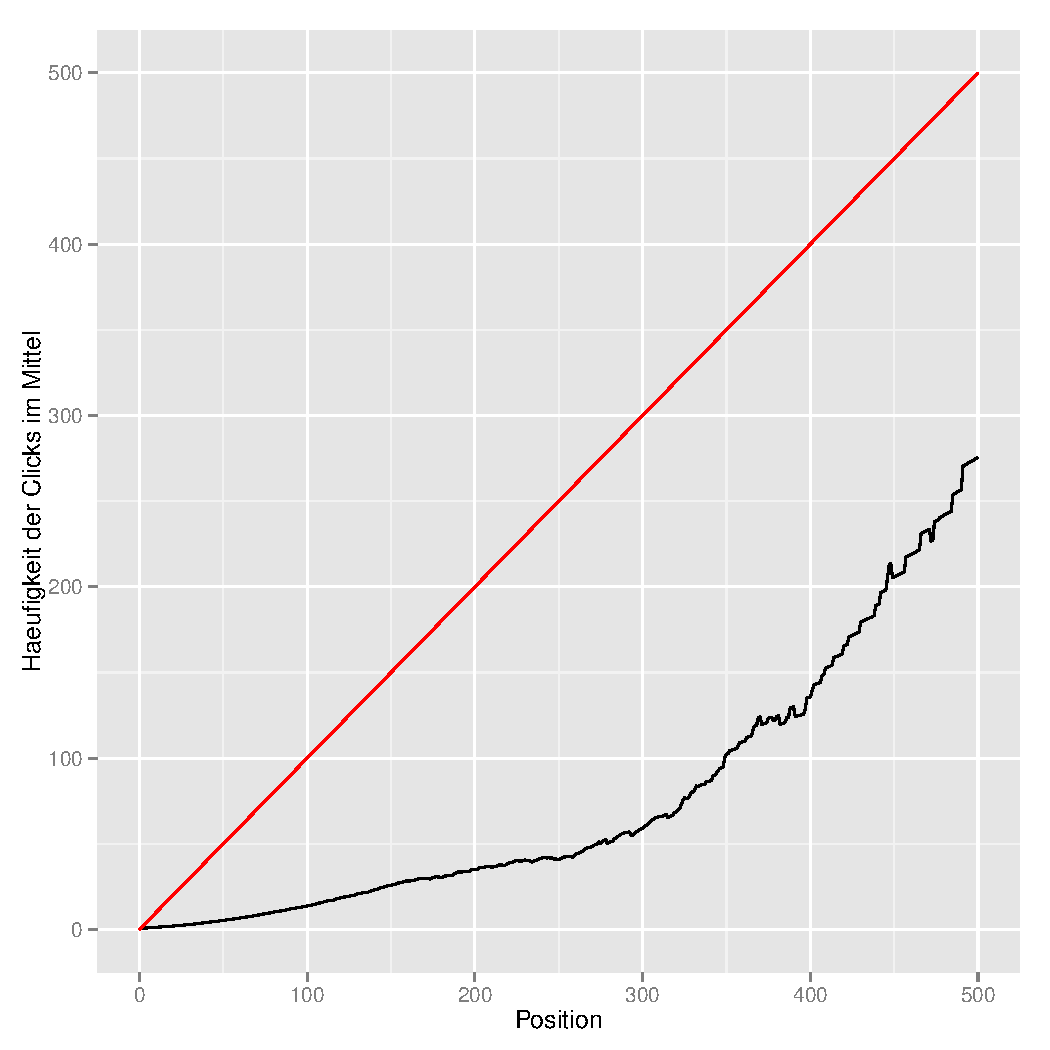
\includegraphics[scale=0.39]{clickCountSucc.pdf}
		\column{4cm}
			\begin{itemize}
				\item Anzahl der Clicks bis zur aktuellen Position
				\item Gemittelt über alle konvertierten Funnels
				\item Mehr \textit{Views} als \textit{Clicks}
			\end{itemize}
	\end{columns}
\end{frame}

%\begin{frame}\frametitle{hasClicked}
	    %\centering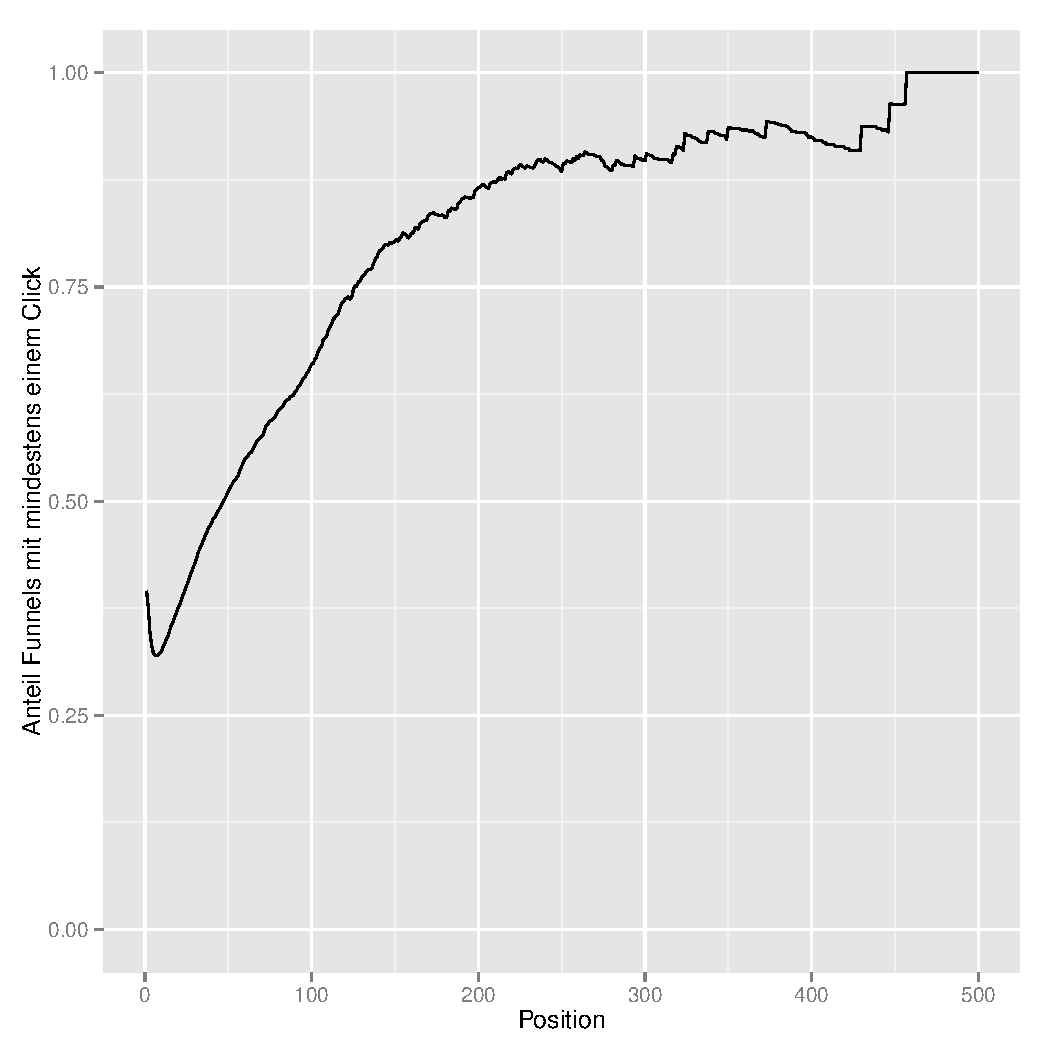
\includegraphics[scale=0.39]{hasClickedSucc.pdf}
%\end{frame}

\begin{frame}\frametitle{Beschreibung der Kampagnen}
	\begin{table}[H]
		\tiny
		\begin{center}
			\begin{tabular}{|l|p{7cm}|}
				\hline \textbf{Kampagne} & \textbf{Beschreibung}\\ \hline
				\hline Affiliate - Partnerprogramm & Partner, die Werbemittel einbinden\\
				\hline Affiliate - Rest & Partner, die Zinsvergleich bereitstellen\\ 
				\hline Direct & Direkte Eingabe von \textit{www.interhyp.de}\\ 
				\hline Display & Bannerschaltungen\\
				\hline E-Mailing & Mails an Interessenten, die schon einen Antrag o.ä. gestellt haben\\
				\hline Generic & Unbezahlter Link\\
				\hline Kooperationen - Focus & \multirow{5}{7cm}{Individuelle Zusammenarbeit mit größeren Partnern}\\
				Kooperationen - Immonet & \\
				Kooperationen - Immoscout24 & \\
				Kooperationen - Immowelt & \\
				Kooperationen - Rest & \\
				\hline Newsletter & Regelmäßige Rundschreiben\\
				\hline SEM - Brand & \multirow{3}{7cm}{Bezahlte Suchergebnisse}\\
				SEM - Remarketing & \\
				SEM - Generisch & \\
				\hline SEO & Unbezahlte Suchergebnisse\\
				\hline Social Media & \textit{facebook} und \textit{gutefrage.net}\\
				\hline
			\end{tabular} 
		\end{center}
	\end{table}
\end{frame}

\begin{frame}\frametitle{campaign}
	\begin{columns}
		\column{7cm}
			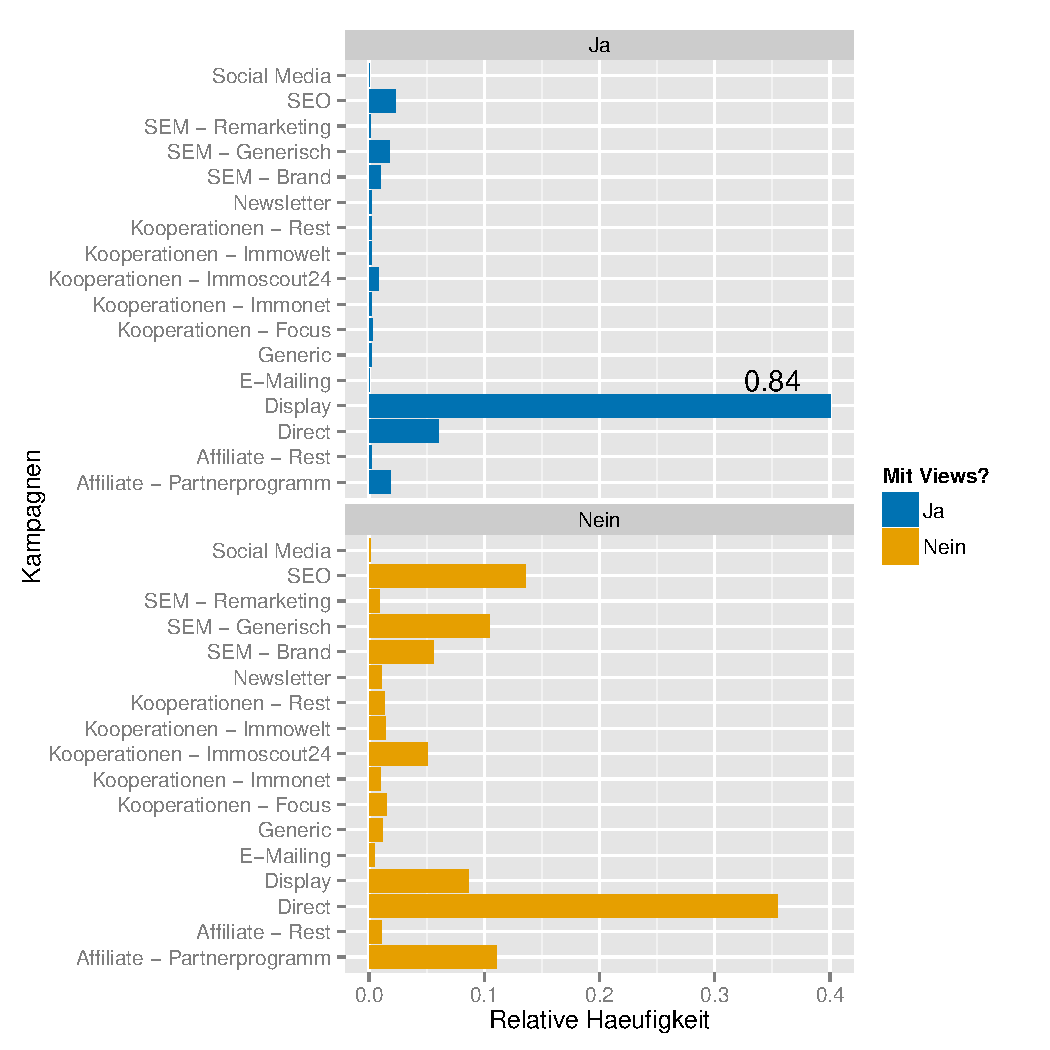
\includegraphics[scale=0.39]{campaignSucc.pdf}
		\column{4cm}
			\begin{itemize}
				\item Hauptsächlich \textit{Display} bei Berücksichtigung der \textit{Views}
				\item Ausgewogenere Verteilung wenn \textit{Views} gelöscht werden
			\end{itemize}
	\end{columns}
\end{frame}

\subsection{Vergleich von konvertierten und nicht-konvertierten Funnels}

%\begin{frame}\frametitle{weekday}
	    %\centering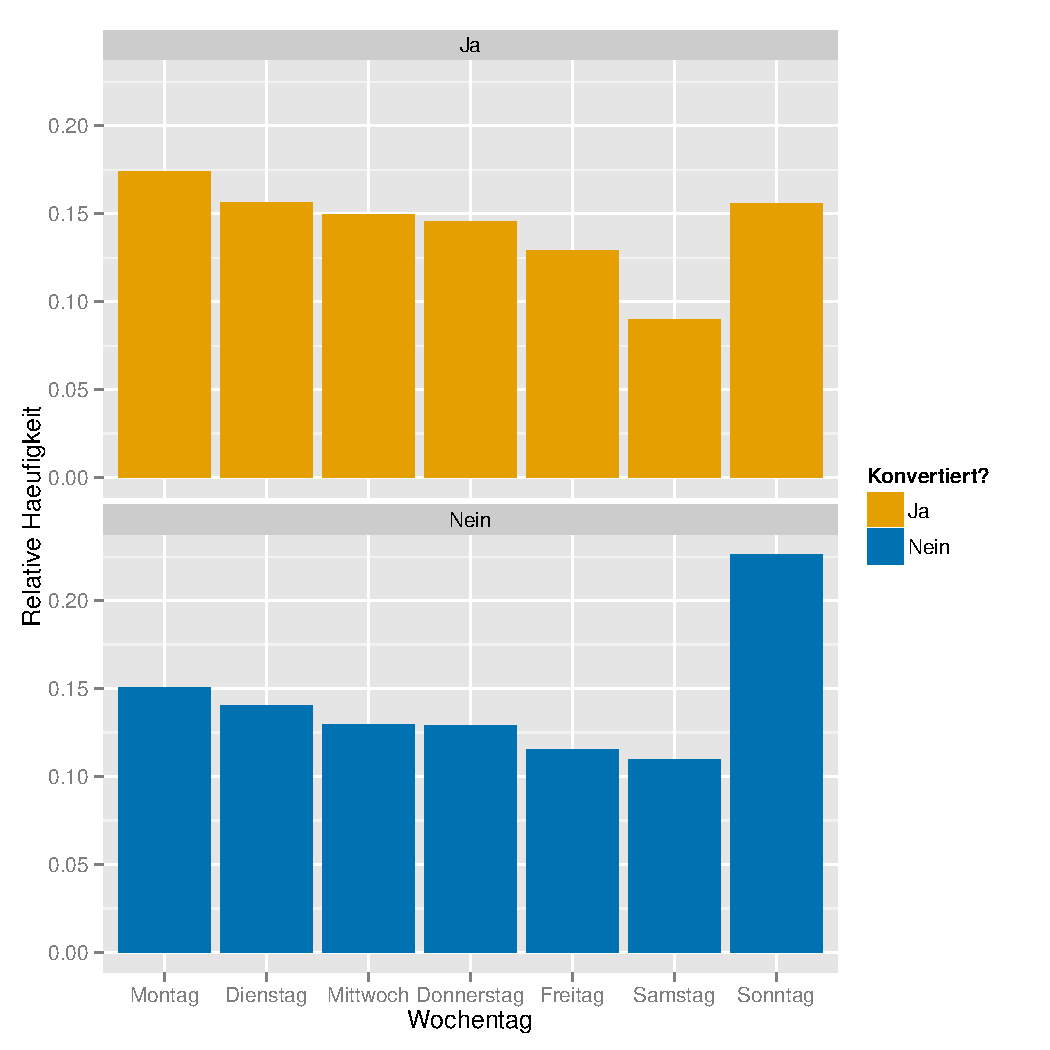
\includegraphics[scale=0.3]{weekday.pdf}
%\end{frame}

%\begin{frame}\frametitle{hour}
	    %\centering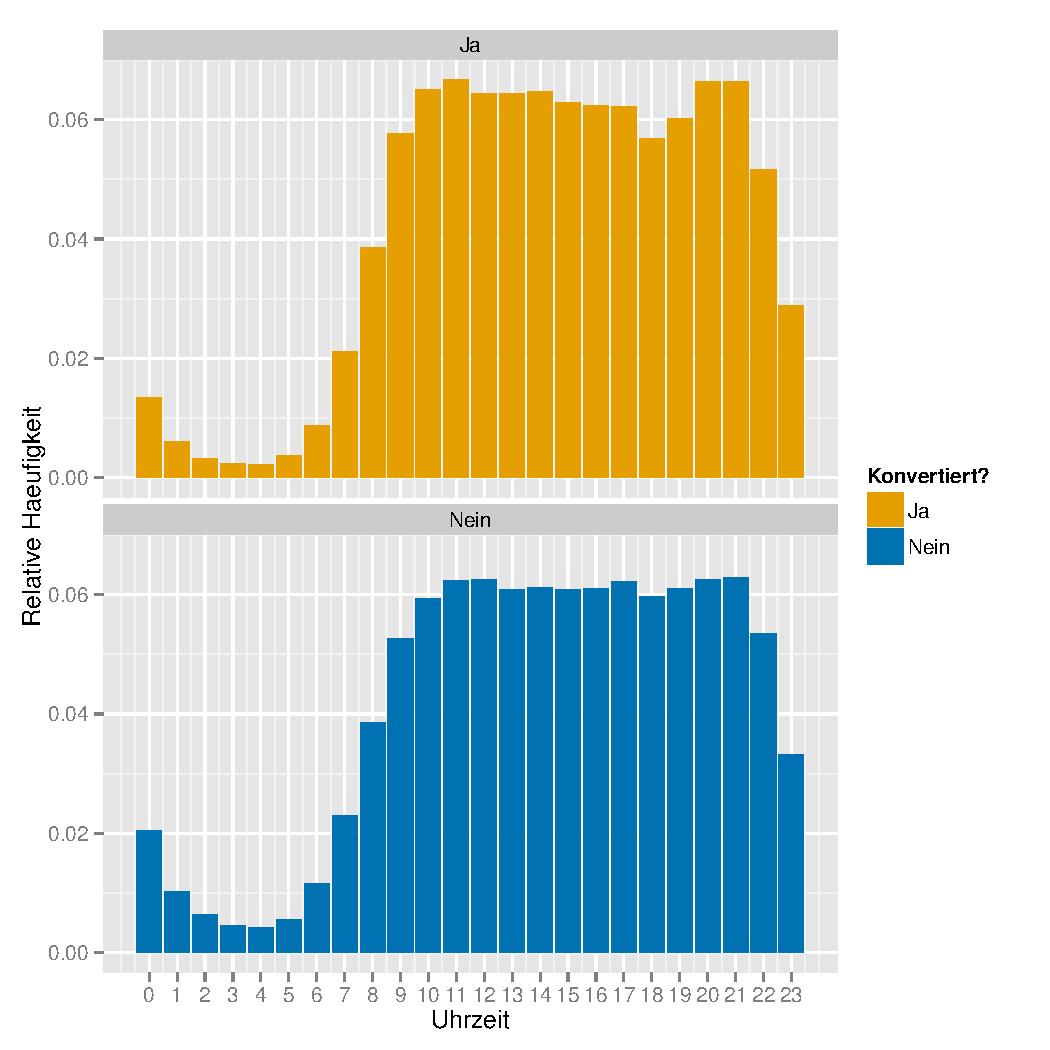
\includegraphics[scale=0.3]{hour.pdf}
%\end{frame}

\begin{frame}\frametitle{campaign}
	\begin{columns}
		\column{7cm}
			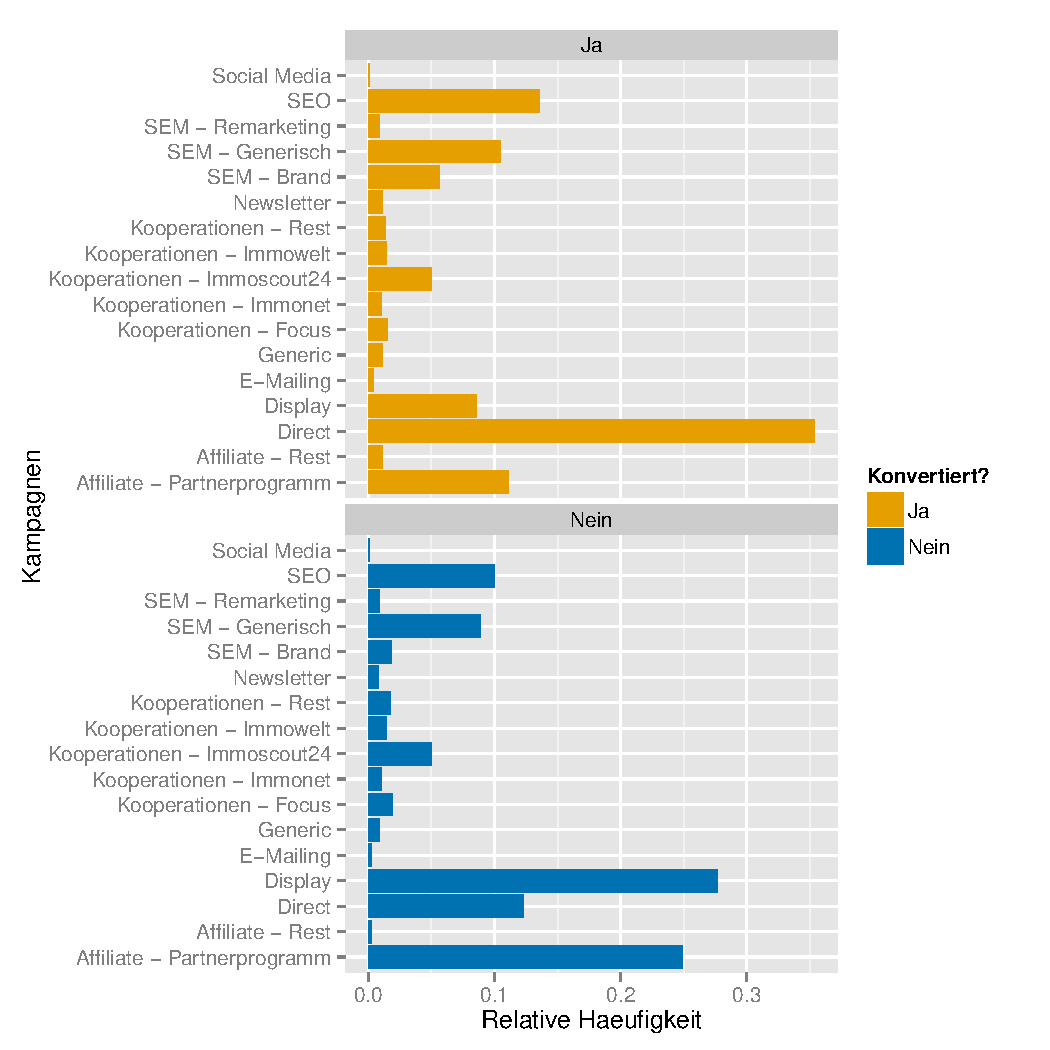
\includegraphics[scale=0.39]{campaign.pdf}
		\column{4cm}
			\begin{itemize}
				\item \textit{Direct} am häufigsten in den konvertierten Funnels
				\item \textit{Display} und \textit{Affiliate - Partnerprogramm} am häufigsten in den nicht-konvertierten Funnels
			\end{itemize}
	\end{columns}
\end{frame}

\begin{frame}\frametitle{funnelLength}
	\begin{columns}
		\column{7cm}
			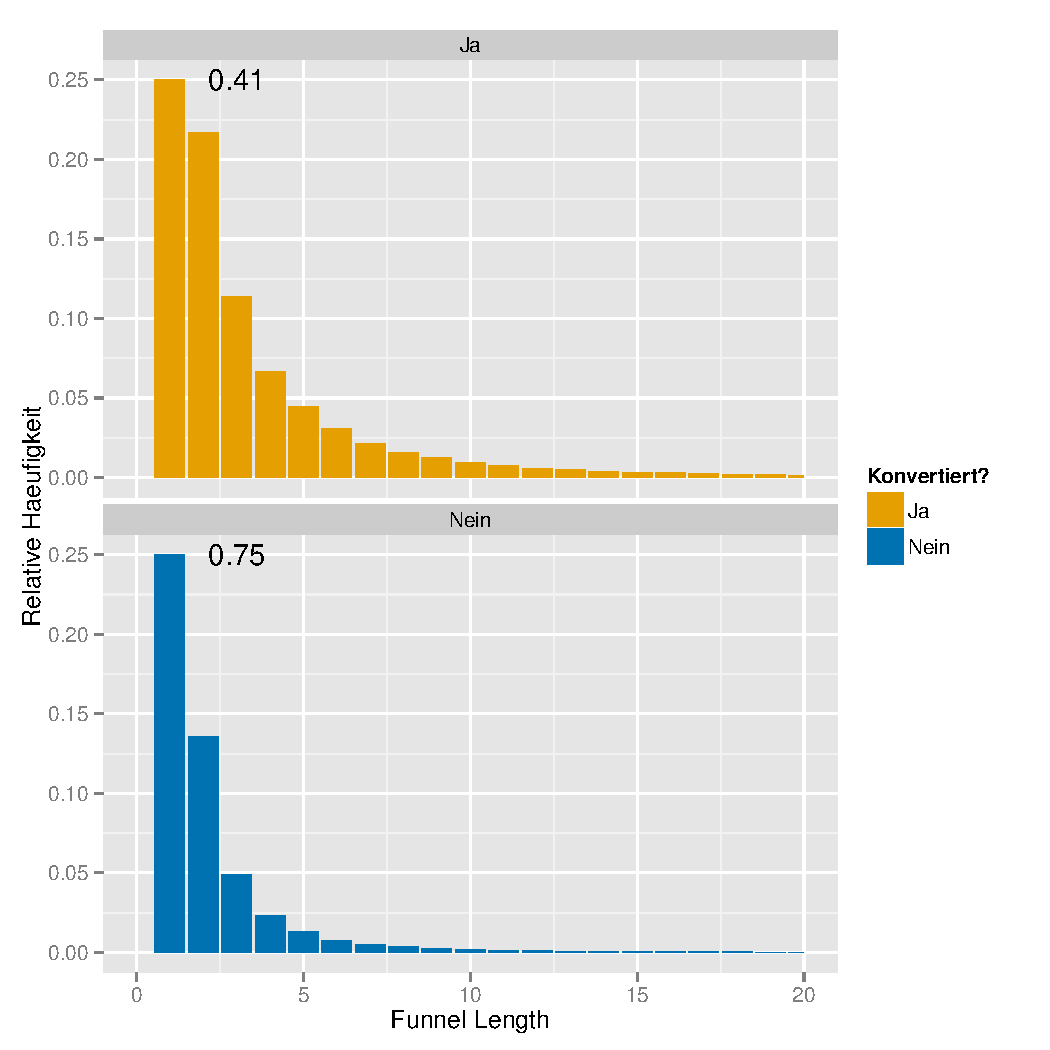
\includegraphics[scale=0.39]{funnelLength_First.pdf}
		\column{4cm}
			\begin{itemize}
				\item Anzahl Kontaktpunkte eines Funnels
				\item Kurze Funnels überwiegen deutlich
			\end{itemize}
	\end{columns}
\end{frame}

\begin{frame}\frametitle{timeSinceFirst}
	\begin{columns}
		\column{7cm}
			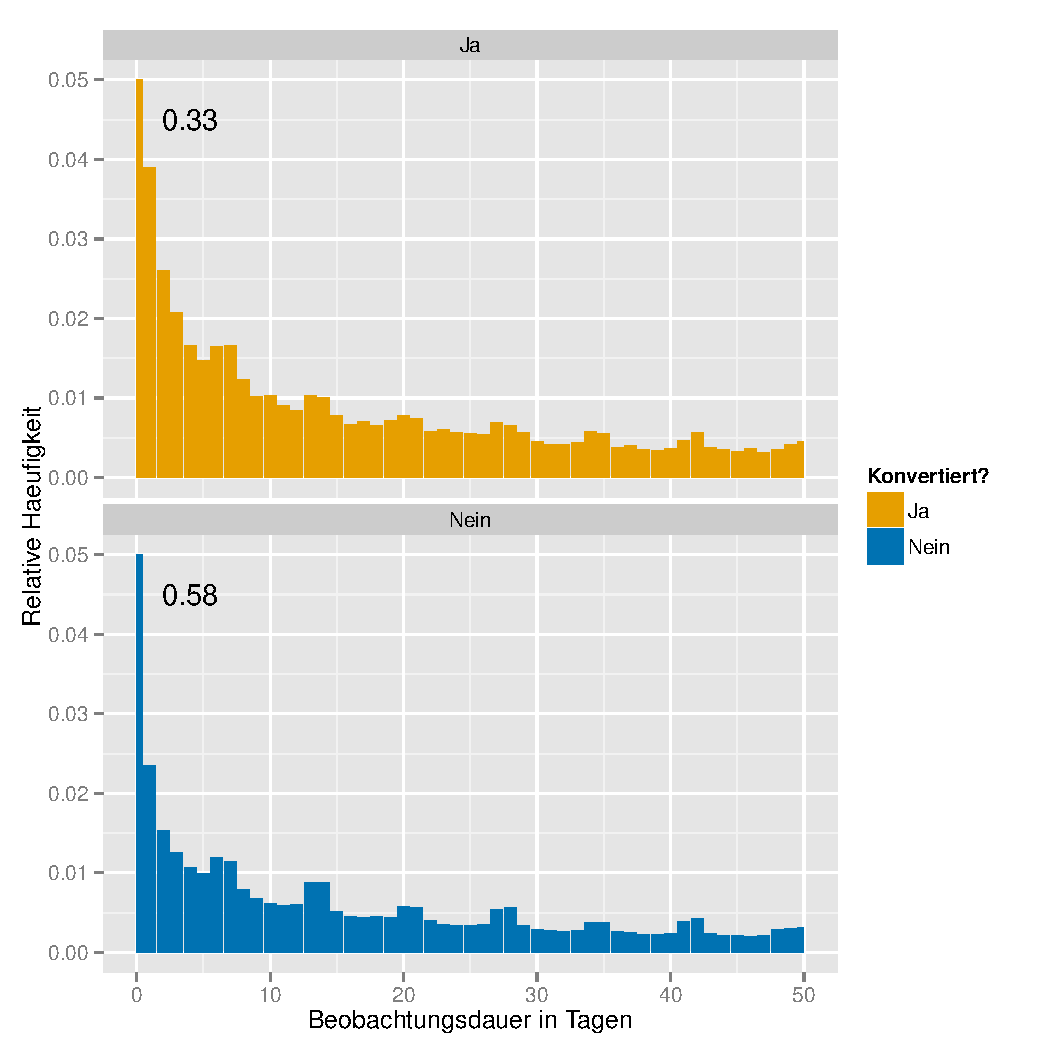
\includegraphics[scale=0.39]{timeSinceFirst_Last.pdf}
		\column{4cm}
			\begin{itemize}
				\item Verstrichene Zeit seit dem ersten Kontaktpunkt
				\item In der Abbildung wird nur der letzte Kontaktpunkt berücksichtigt
				\item Funnels mit Länge $1$ unberücksichtigt
				\item \textit{timeSinceLast}: Verstrichene Zeit seit dem vorherigen Kontaktpunkt
			\end{itemize}
	\end{columns}
\end{frame}

%\begin{frame}\frametitle{timeSinceLast}
	%\begin{columns}
		%\column{7cm}
			%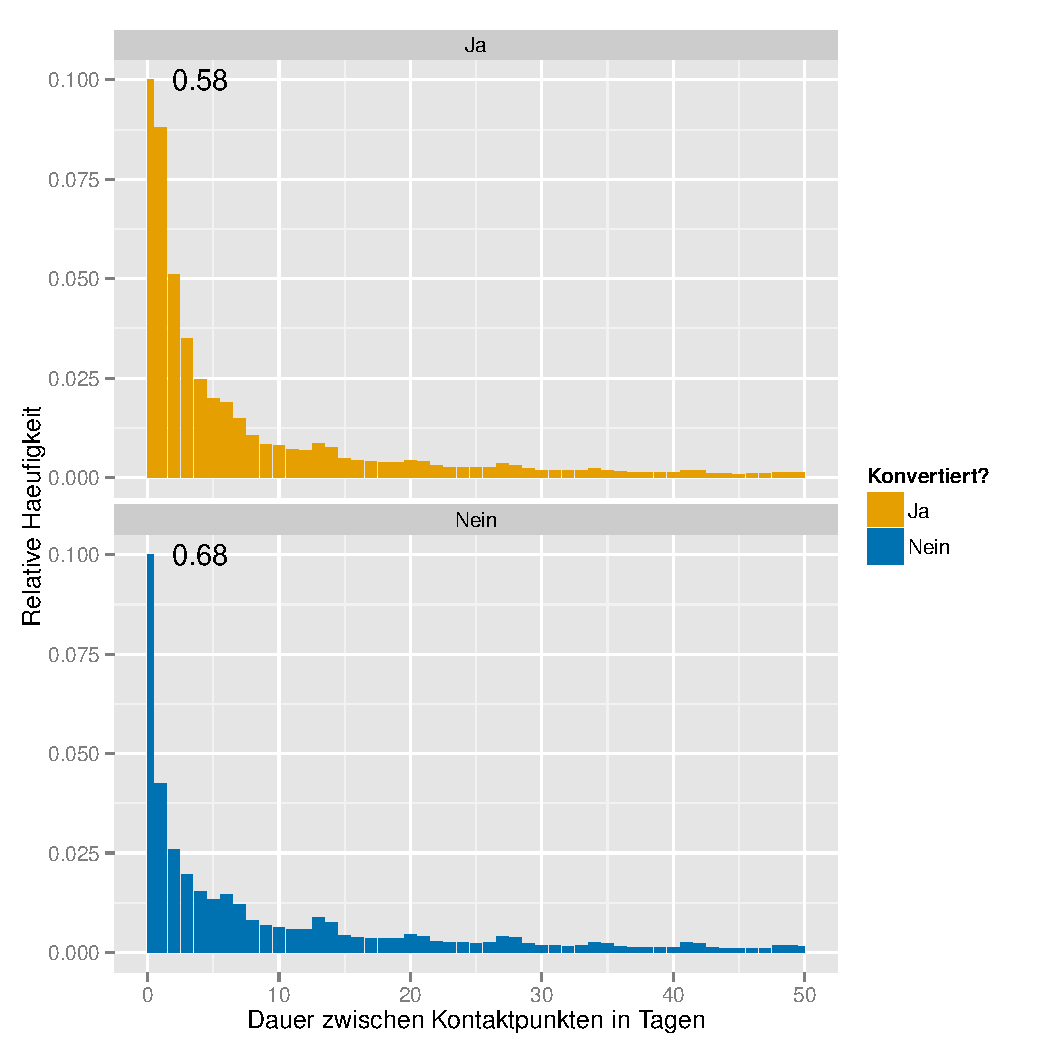
\includegraphics[scale=0.39]{timeSinceLast.pdf}
		%\column{4cm}
			%\begin{itemize}
				%\item 
			%\end{itemize}
	%\end{columns}
%\end{frame}

\begin{frame}\frametitle{freq}
	\begin{columns}
		\column{7cm}
			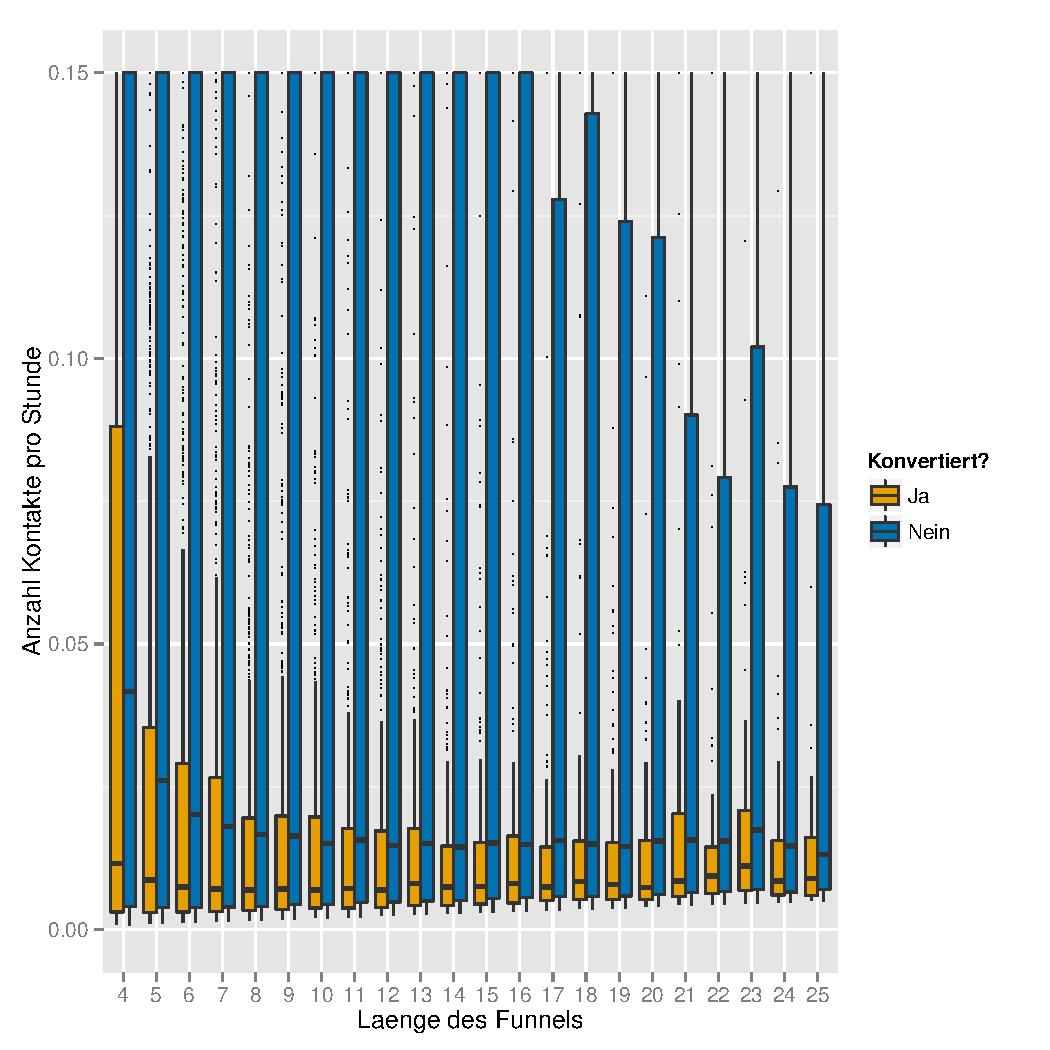
\includegraphics[scale=0.39]{freq.pdf}
		\column{4cm}
			\begin{itemize}
				\item \textit{funnelLength} dividiert durch Gesamt-Beobachtungsdauer in Stunden
				\item Frequenzen in nicht-konvertierten Funnels höher
			\end{itemize}
	\end{columns}
\end{frame}

\section{Tutorial zu Gephi}\label{tutorial}
\subsection*{Erläuterungen der Dateien}
In diesem Teil wird ein Tutorial zu dem Open Source Programm Gephi beschrieben. Diese Program liest hauptsächlich .gexf Dateiformate ein und erstellt dann aus diesen ein Netzwerk aus Knoten und Kanten. gexf Dateien sind in einem speziellen XML Format geschrieben und können sehr viele Informationen und Attribute übergeben. Die Dateien für dieses Tutorial wurden in R mit den Skripten gexf.R und gexf\_support.R erstellt. Mit den Skripten können verschiedene Parameter und Attribute übergeben werden, wie zum Beispiel die farbliche Kodierung der Knoten und die Gewichtung der Kanten. Das Format der bearbeiteten Netzwerke sind .gephi Dateien, die ausschlieslich in Gephi eingelesen werden können. In diesen sind dann typischerweise Layouts und gefilterte Graphen gespeichert. Die nachfolgende Tabelle gibt eine Übersicht über die .gexf und .gephi Dateien, die im elektronischen Anhang bereits vorhanden sind und mit Hilfe deren das Tutorial beschrieben wird.


\begin{table}[H]
    \begin{center}
        \begin{tabular}{|c|p{7cm}|} 
            \hline  relative\_ausgaenge.gexf  & unbearbeiteter Graph, die ersten 100 Position sind als Knoten dargestellt, Gewichtung der Kanten sind die relativen Ausgaenge \\
            \hline  relative\_ausgaenge\_pos\_10.gexf  & unbearbeiteter und gefilteter Graph, die ersten 10 Position sind als Knoten dargestellt , Gewichtung der Kanten sind die relativen Ausgaenge \\
            \hline  relative\_ausgaenge\_pos\_10\_Layout.gephi  & bearbeiteter Graph mit Layout, die ersten 10 Position sind als Knoten dargestellt , Gewichtung der Kanten sind die relativen Ausgaenge und die Knoten sind nach relativen Haeufigkeiten gewichtet\\
            \hline  relative\_gaenge.gexf  & unbearbeiteter Graph, die ersten 100 Position sind als Knoten dargestellt, Gewichtung der Kanten sind die relativen Ausgaenge \\  
            \hline  relative\_eingaenge\_pos\_10.gexf  & unbearbeiteter und gefilteter Graph, die ersten 10 Position sind als Knoten dargestellt , Gewichtung der Kanten sind die relativen Ausgaenge \\
            \hline relative\_eingaenge\_pos\_10\_Layout.gephi  & bearbeiteter Graph mit Layout, die ersten 10 Position sind als Knoten dargestellt , Gewichtung der Kanten sind die relativen Ausgaenge und die Knoten sind nach relativen Haeufigkeiten gewichtet \\     
            \hline
        \end{tabular} 
    \end{center}
    \caption{Übersicht der Gephi Dateien}\label{Gephi_dateien}
\end{table}

\subsection*{Erste Schritte mit Gephi}
Nach der Installation und öffnen des Programs, kann man über $ \rightarrow $ File $ \rightarrow $ Open, die Dateien öffnen und bei dieser Datenlage ist der Import Report zu vernachlässigen. Die folgende Abbildung zeigt den Workspace nach dem Laden der relative\_ausgaenge.gexf Datei. Im lila Kasten sind die einzelnen Bearbeitungsmodi von Gephi. Overview ist dafür gedacht den Graphen zu bearbeiten und mit einem Layout zu versehen. Im Data Labratory kann man einzelne Knoten und Kanten bearbeiten und neue Attribute hinzufügen. Der Preview ist dann eine Vorschau von der Datei die exportiert wird und kann hierzu auch noch weiter verändert werden. Außerdem befindet sich hier der Export der Graphen.Gelb markiert sind die Daten, die als Knoten und Kanten dargestellt sind. Diese quaderförmige Struktur besitzt der Graph nur am Anfang und wird durch den blauen Kasten auf der linken Seite verändert. Hier kann man den gewünschten Algorithmus auswählen, der die Position der Knoten berechnet und durch Parameter eingestellt werden kann. Zum Beispiel haben wir die Parameter \textit{Edge Weight Influence}, dass den Einfluss der Gewichtung der Kanten steuert, auf $ 0.1 $. Das \textit{Scaling} , die Größe des Graphen , wurde auf $ 200 $ festgelegt und \textit{Approximate Repulsion} , zuständig für die Konvergenz des Graphen, wurde nicht makiert damit es einen größeren und übersichtlicheren Graphen ergibt. Am Ende des Algorithmus wurde noch das \textit{Prevent Overlap} aktiviert um keine Überlappungen der Knoten zu haben. \\
Um das Layout und die Struktur weiter zu beeinflußen , kann man in dem linken roten Kasten die Größe der Kanten und der Knoten definieren, dabei muss der rote Diamant ausgewählt werden und ein Gewichtungsattribut ausgewählt werden, in unserem Fall die Variable \textit{relative}, die den relativen Häufigkeiten der auftretenden Knoten in einer Position entspricht. Im grünen Feld daneben befinden sich die Optionen für die Maus, wie zum Beispiel die voreingestellte Fähigkeit, dass man Knoten manuell im Graphen bewegen und positionren kann. Aber auch die letzte Option ist hilfreich, mit der man durch einen Klick auf einen Knoten, dessen beinhaltete Information ersehen kann. Die Boxen auf der linken Seite dienen hauptsächlich dazu den Graphen zu filtern und in einen neuen Workspace zu exportieren.\\
Im linken Roten Feld kann man \textit{Statistics} und \textit{Filters} anwenden, bei den Filtern handelt es sich um die übergebenen Attribute nach denen Gefilter werden kann. Bei \textit{Partition} befindet sich die Position als Attribute, mit der eingestellt werden kann welche Position im Graphen angezeigt werden kann. Diesen Filter muss man dann in den grünen Kasten ziehen um dann die Auswahlmöglichkeiten im blauen Kasten zu bekommen. Hier kann kann man dann die gewünschten Position dann auswählen und mittels dem Button \textit{Filter} aktivieren. Desweiteren kann man auch einen \textit{subfilter}, also einen zweiten Filter gleichzeitig anwenden und hier empfiehlt sich dann das \textit{Edge Weight}. Generell empfiehlt es sich, dass man erst den Graphen nach seinen Interessen filtert und dann den Layout Algorithmus anwendet, da sich dieser je nach Filterung anpasst. Weitere hilfreiche Features des Programs befinden sich in der Fußzeile des Workspaces, wie zum Beispiel das ein- oder ausblenden von Knotenlabels mithilfe des großen \textit{T} oder der Screenshot Funktion.

\begin{figure}[H]
    \centering
    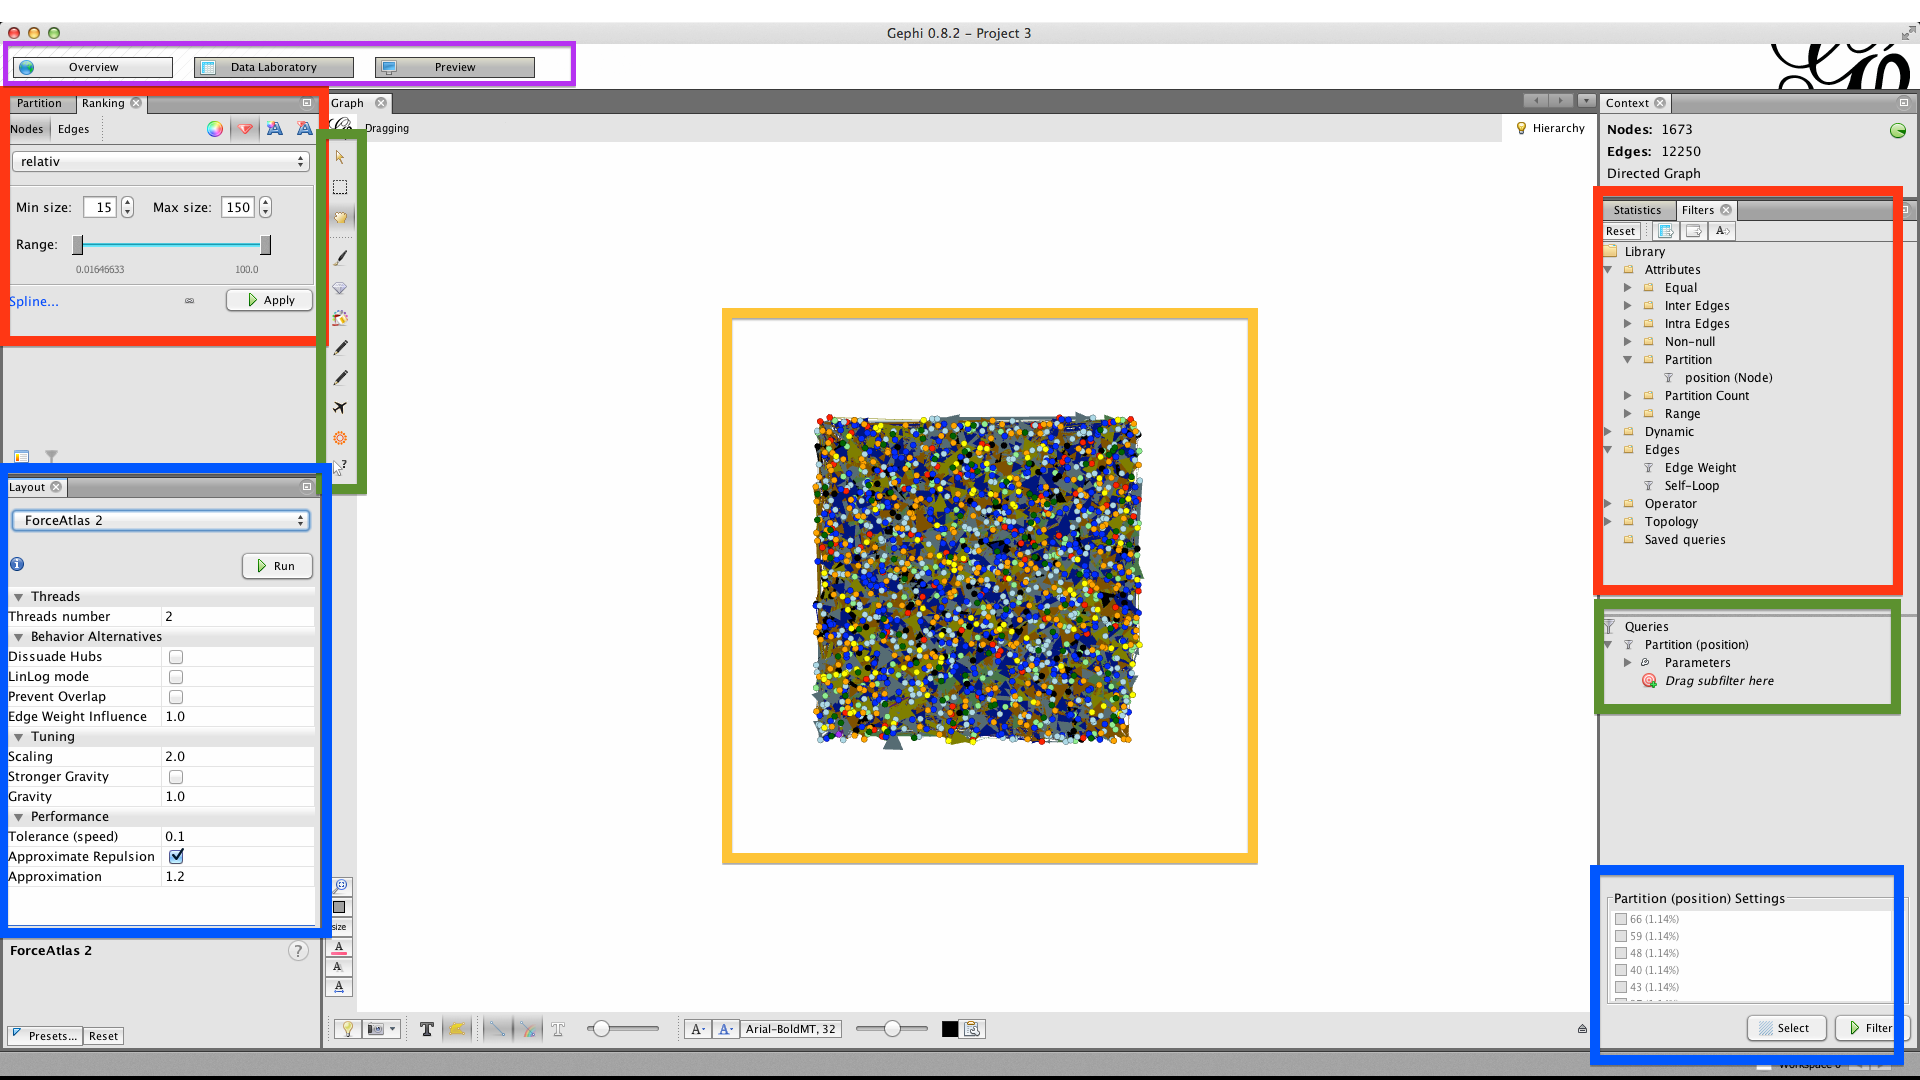
\includegraphics[scale=0.25]{workspace.png}
    \caption[workspace]{Der Workspace in Gephi}
    \label{workspace}
\end{figure}


\subsection*{Ergebnisse und Interpretation mit Gephi}
Um Ergebnisse und Erkenntnisse aus den erstellten Grafiken zu ziehen und zu gewinnen, kann man durch das scrollen in den Graphen hineinzoomen und durch Halten des Rechtsklickes durch den Graphen durch zu ziehen navigieren. Wenn man dann eine aussagekräfige Position im Graphen gefunden hat, wird durch das drüber schweben der Maus über einen Knoten die Verbindung von und zu diesem Knotenpunkt ersichtlich. In der Grafik unten ist dieser Fall beispielsweise an der Position 7 dargestellt. In diesem Fall wurde der Success Knoten ausgewählt und die relativen Ausgänge als Gewichtung. Hier sieht man, aber auch dass es Sinn macht weiterhin Filter zu benutzen um bedeutendere Ergebnisse zu erzielen.


\begin{figure}[H]
    \centering
    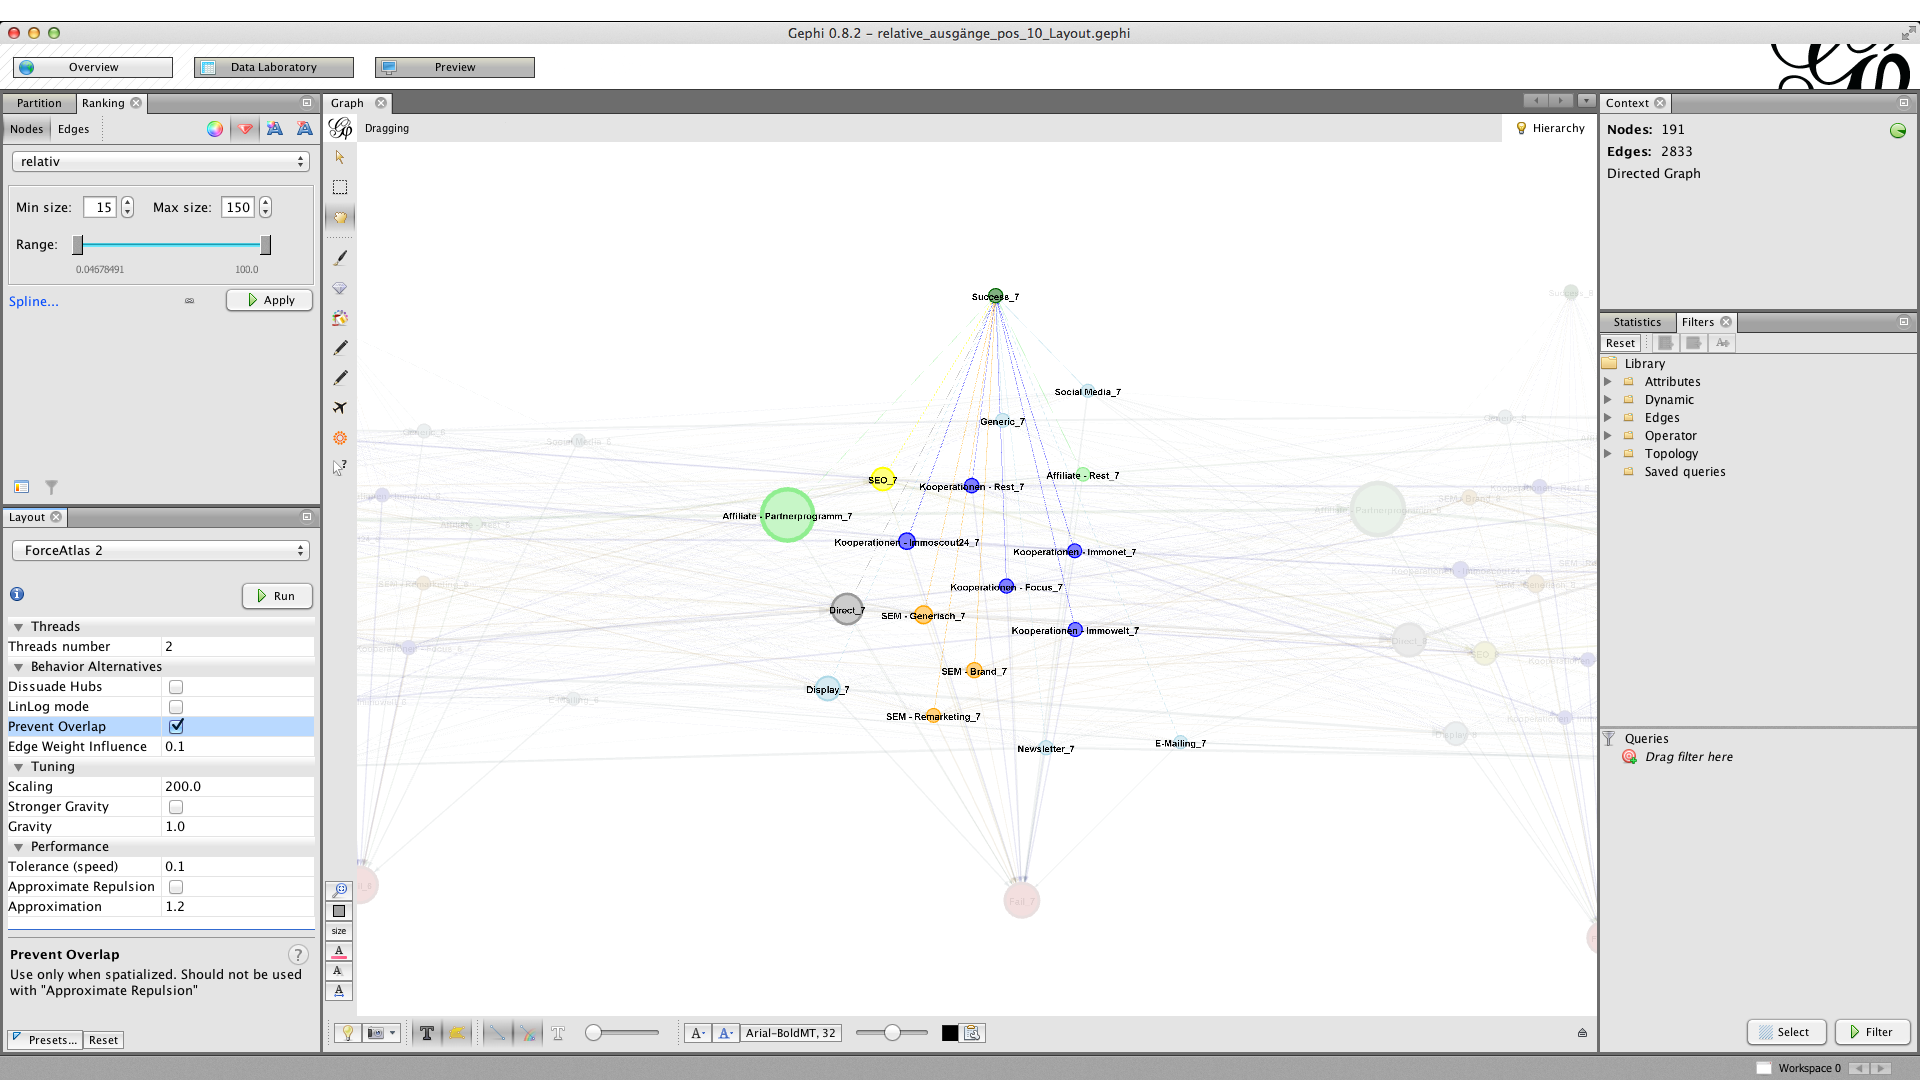
\includegraphics[scale=0.25]{ergebnis_gephi.png}
    \caption[ergebnis]{Ergebnisse in Gephi}
    \label{ergebnis}
\end{figure}


\subsection*{Export in Gephi}
Wenn man dann einen Graphen soweit bearbeitet hat und das Gesamtergebnis exportieren will, kann man das in dem Reiter Preview machen. Nützliche Einstellungen hier sind zum Beispiel im lila Feld \textit{Rescale Weight}, damit die Kanten nicht zu dick sind und das ausstellen von \textit{Curved}, weil diese Funktion zwar den Graphen schön aussehen lässt, aber unübersichtlicher macht. In der grünen Box muss man nach jeder Einstellung den \textit{Refresh} Button klicken und kann zusätzlich den Graphn als SVG-,PDF- oder PNG-Format abspeichern.

\begin{figure}[H]
    \centering
    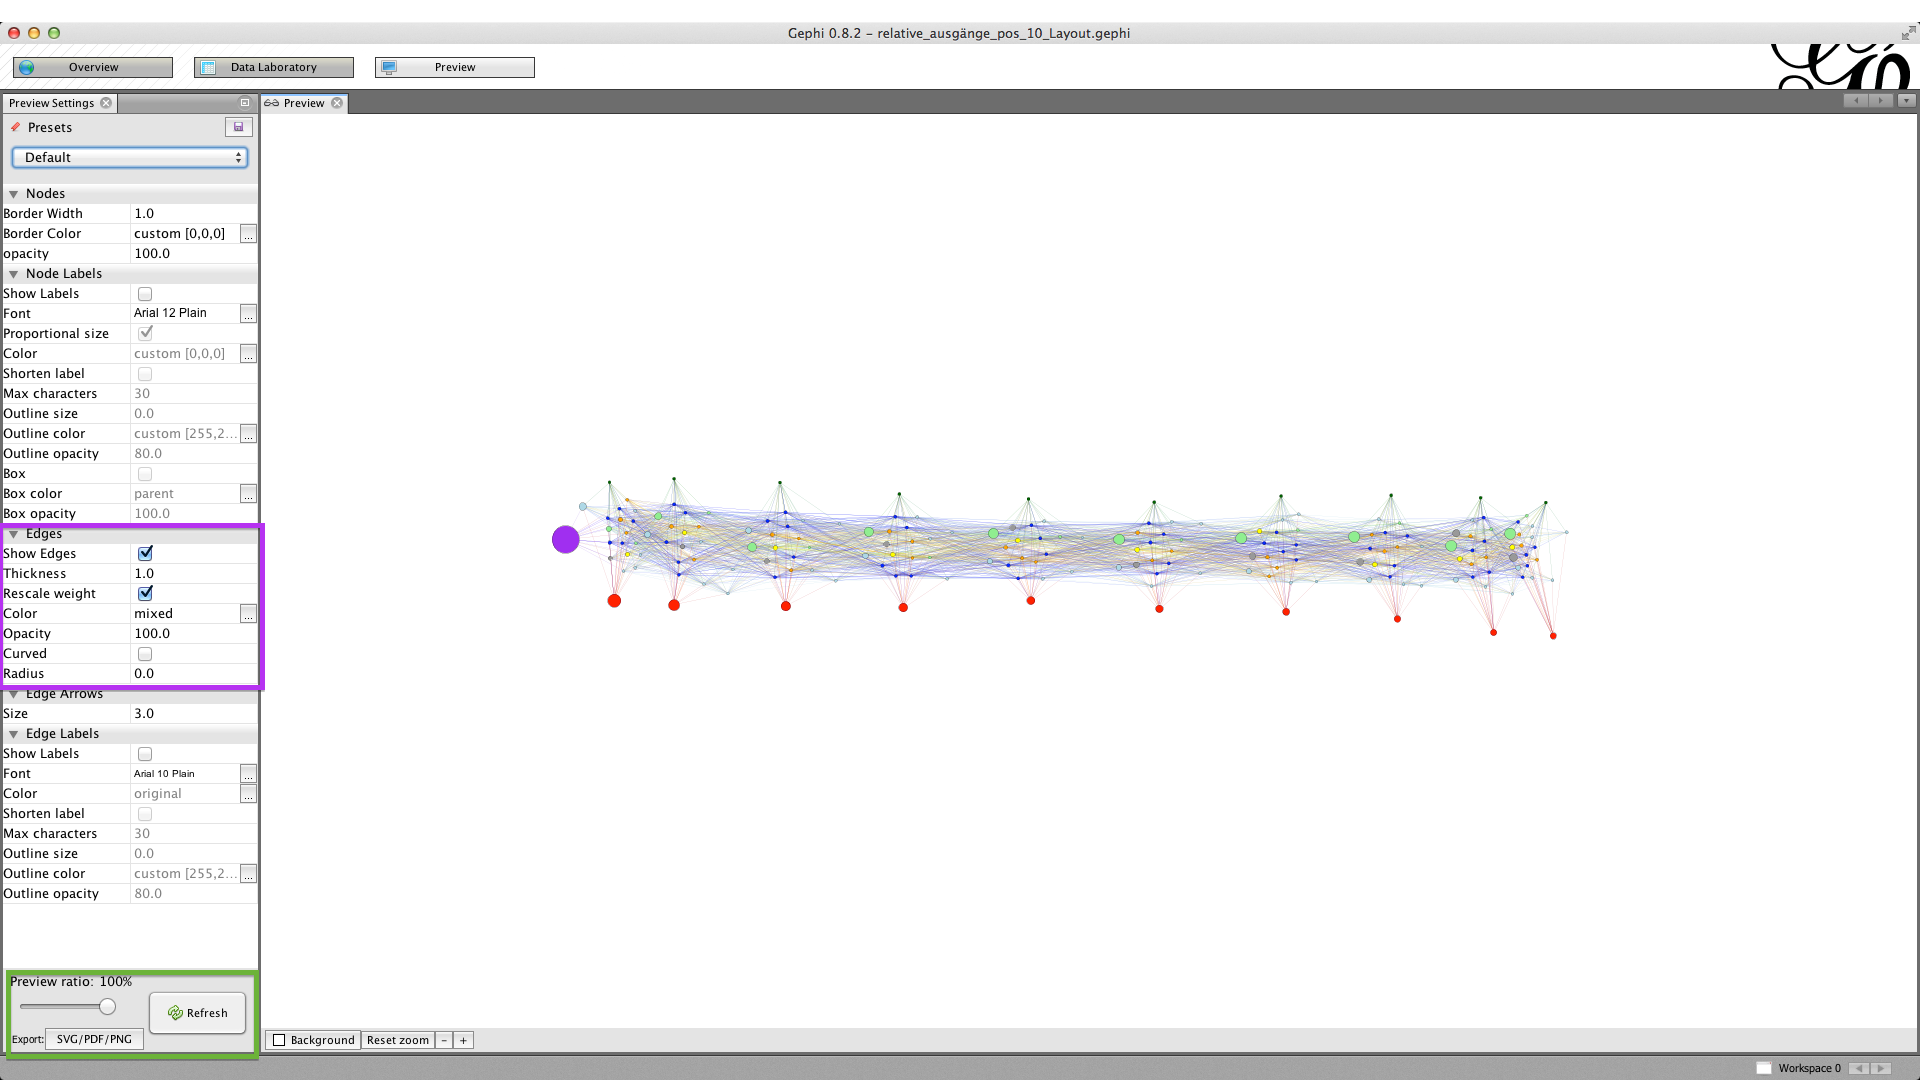
\includegraphics[scale=0.25]{Preview.png}
    \caption[export]{Der Export in Gephi}
    \label{export}
\end{figure}




\section{Zeitdiskretes Survival-Modell}\label{survival}

\subsection{Lebensdauer-Modell}\label{secModel1}

Aufgrund der in Kapitel \ref{datenlage} beschriebenen Datenlage erscheint die Anwendung eines Modells aus dem Feld der Lebensdaueranalyse intuitiv. Es wird die Zeit bis zu einem Ereignis betrachtet, welches in diesem Fall das Ausfüllen eines Online-Antrages ist. Der potentielle Kunde befindet sich während der Beobachtungsspanne im transienten Zustand bis er durch die Konvertierung in den absorbierenden Zustand wechselt, an dem die Beobachtung endet. Tritt am Ende der Beobachtung keine Konvertierung ein, so spricht man von einer Rechtszensierung.\\
Die Position gibt die Nummer des Kontaktpunktes an und bildet die Zeitachse des Modells. Das heißt, es handelt sich um ein zeitdiskretes Modell und die Zielvariable $y_{ip}$ (\ref{zielvar}) nimmt den Wert Eins an, wenn Kunde $i$ an der Position $p$ konvertiert ist. Für alle vorherigen Positionen eines konvertierten Funnels und für alle Positionen eines nicht-konvertierten Funnels nimmt $y_{ip}$ den Wert Null an. $N_p$ ist die Anzahl der Beobachtungen an Position $p$. Diese nimmt mit steigendem $p$ ab, da in jeder Position Funnels konvertieren oder Beobachtungen ohne Konvertierung enden. Deshalb wird das Modell nur auf die ersten $25$ Positionen angewendet, da für spätere Positionen nicht ausreichend konvertierte Funnels vorliegen.\\
\begin{align}
	y_{ip} = \begin{cases} 1 & \text{Beobachtung } i \text{ konvertiert an Position } p\\
												 0 & \text{sonst} 
					 \end{cases} \text{, } p=1,...,25 \text{, } i=1,...,N_p \label{zielvar}
\end{align}
Das Modell schätzt die Hazardrate $\lambda_{ip}$ (\ref{haz}), das heißt die Wahrscheinlichkeit, dass Beobachtung $i$ an Position $p$ konvertiert unter der Bedingung, dass die Länge des Funnels von Beobachtung $i$ größer oder gleich $p$ ist, was lediglich bedeutet, dass für Beobachtung $i$ an Position $p$ überhaupt noch ein Kontaktpunkt vorliegt. Außerdem wird auf die Features $x_{ip}$ bedingt, die später noch näher erläutert werden.
\begin{align}
	\lambda_{ip} = P(y_{ip}=1|funnelLength_i \geq p, x_{ip}) \label{haz}
\end{align}
Die Hazardrate wird mittels eines Logit-Modells (\ref{logit1}-\ref{logit2}) mit der Zielvariable $y_{ip}$ an jeder Position $p$ seperat geschätzt. Die Annahmen des Modells sind, dass die $y_{ip}|x_{ip}$ unabhängig Bernoulli-verteilt sind mit der Hazardrate $\lambda_{ip}$ als Parameter und der Erwartungswert wird anhand der Responsefunktion $h$ mit der Prädiktorfunktion $f_{p}$ verknüpft.
\begin{align}
	y_{ip}|x_{ip} &\stackrel{ind}{\sim} Bin(1, \lambda_{ip}) \label{logit1} \\
	E(y_{ip}|x_{ip}) = P(y_{ip} = 1|x_{ip}) = \lambda_{ip} &= h(f_{p}(x_{ip})) = \frac{\exp(f_{p}(x_{ip}))}{1+\exp(f_{p}(x_{ip}))}\label{logit2}
\end{align}
Aus diesen Annahmen lassen sich Likelihood (\ref{lik}) und Log-Likelihood (\ref{loglik}) des Modells ableiten.
\begin{align}
	L(\lambda_{ip}) &= \prod_{i=1}^{N_p} \lambda_{ip}^{y_{ip}} (1-\lambda_{ip})^{1-y_{ip}} \label{lik} \\
	l(\lambda_{ip}) &= \ln(L(\lambda_{ip})) = \sum_{i=1}^{N_p} (y_{ip} \ln(\lambda_{ip}) + (1-y_{ip}) \ln(1-\lambda_{ip})) \notag \\
	&= \sum_{i=1}^{N_p} (y_{ip} f_p(x_{ip}) - \ln(1+\exp(f_p(x_{ip})))) \label{loglik}
\end{align}
Damit ergibt sich der binomielle Verlust aus der negativen Log-Likelihood (\ref{binVer}) und das Logit-Modell ist lösbar durch die Minimierung dieses Verlusts.
\begin{align}
	L(y_{ip},f_p(x_{ip})) = -\sum_{i=1}^{N_p} (y_{ip} f_p(x_{ip}) + \ln(1+\exp(f_p(x_{ip}))))
\end{align}
Um ein gutes Prognose-Modell zu entwickeln, wird eine Ensemble-Methode angewendet, die im nächsten Abschnitt vorgestellt wird.

\subsection{Stochastic Gradient Boosting}\label{secModel2}

\subsubsection*{Algorithmus}

Stochastic Gradient Boosting ist eine Ensemble-Methoden, die durch mehrfache Anwendung des sogenannten Basis-Lerners ein Ensemble von Schätzern für eine Prognosefunktion liefert. Durch Aggregation der Schätzer erhält man die endgültige Prognosefunktion. Ein sehr beliebter Basis-Lerner sind Stümpfe, das heißt Bäume mit nur einem Split. Einige Vorteile von Bäumen sind, dass sie mit kategoriellen Features, Ausreißern und fehlenden Werten umgehen können. Außerdem wird der schwachen Prognoseleistung von Bäumen durch die Kombination mit Boosting entgegen gewirkt.\\
Gesucht ist also eine Prognosefunktion, die den Erwartungswert einer Verlustfunktion minimiert. Als Verlustfunktion wird der binomielle Verlust (\ref{binVer}) verwendet, wobei sich die Prädiktorfunktion wie folgt ergibt.
\begin{align}
	f(x_{ip}) =& \text{offset}(\hat{\lambda}_{i,p-1}) + \notag \\
						 &f_{weekday,p}(\text{weekday}_{ip}) + \notag \\
						 &f_{hour,p}(\text{hour}_{ip}) + \notag \\
						 &f_{campaign,p}(\text{campaign}_{ip}) + \notag \\
						 &f_{campaignLast,p}(\text{campaign}_{i,p-1}) + \notag \\
						 &f_{campaignLast2,p}(\text{campaign}_{i,p-2}) + \notag \\
						 &f_{timeSinceLast,p}(\text{timeSinceLast}_{ip}) + \notag \\
						 &f_{timeSinceFirst,p}(\text{timeSinceFirst}_{ip}) \label{praediktor}
\end{align}
Der Prädiktor ist also eine additive Funktion von Treppenfunktionen der sieben verwendeten Features und einem offset. Hier sei nochmal darauf hingewiesen, dass Features wie \textit{hasClicked} oder \textit{clickCount} nicht verwendet werden können, da die Views aufgrund der Problematik der Datenerhebung nicht berücksichtigt werden. Die verwendeten Einflussgrößen sind also der Wochentag und die Stunde des jeweiligen Kontaktpunktes, die Kampagne des aktuellen und der letzten zwei Kontakte, sowie die Dauer seit dem vorherigen Kontaktpunkt und die Gesamtdauer seit dem ersten bis zum jetzigen Kontakt. Die Funktionen $f_{.,p}$ können theoretisch für verschiedene Positionen komplett unterschiedliche Formen annehmen. Es sei ausdrücklich darauf hingewiesen, dass $f_{campaignLast,p}(\textit{campaign}_{i,p-1})$ und $f_{campaign,p-1}(\textit{campaign}_{i,p-1})$ zwei unterschiedliche Funktionen sind. Erstere gibt den Einfluss der Art des vorherigen Kontaktpunktes auf die Konvertierungswahrscheinlichkeit an der Position $p$ wieder und zweitere den Einfluss der Art des aktuellen Kontaktpunktes auf die Konvertierungswahrscheinlichkeit an der Position $p-1$. Unter der Annahme, dass der Einfluss der Features an den verschiedenen Positionen ähnlich ist, fließt zusätzlich noch die Vorhersage des Modells der vorherigen Position als offset mit ein. Dadurch konnten die Ergebnisse besonders an späteren Positionen, an denen weniger Daten vorhanden sind, deutlich verbessert werden. Ergebnisse ohne offset sind im elektronischen Anhang zu finden.\\
Der offset fällt für Position eins weg, da es noch keine Vorhersagen eines vorherigen Modells gibt. Außerdem sind für Position eins die Features \textit{campaignLast}, \textit{campaignLast2}, \textit{timeSinceLast} und \textit{timeSinceFirst} offentsichtlich noch nicht vorhanden, so dass diese ebenfalls wegfallen. An Position zwei ist \textit{campaignLast2} noch nicht vorhanden und \textit{timeSinceLast} und \textit{timeSinceFirst} sind hier identisch, so dass nur eine der beiden berücksichtigt wird. Ab Position Drei ergibt sich der Prädiktor dann exakt so wie in (\ref{praediktor}) dargestellt.\\
\floatname{algorithm}{Algorithmus}
\begin{algorithm}
\caption{Gradient Boosting}\label{alg}
\label{gradboosting}
\begin{algorithmic}
\STATE Setze Startwert für $f_{0p}(x_{ip})$
\FOR{$m=1:n.trees$}
	\STATE Setze $\lambda_{ip}(x_{ip}) = \frac{\exp(f_{m-1,p}(x_{ip}))}{1+\exp(f_{m-1,p}(x_{ip}))}$
	\FOR{$i=1:N_p$} 
		\STATE $r_{imp} = - \frac{\partial L(y_{ip},f_{m-1,p}(x_{ip}))}{\partial f_{m-1,p}(x_{ip})} = y_{ip} - \lambda_{ip}(x_{ip})$
	\ENDFOR
	%\STATE Fit a regression base learner to the pseudo-residuals $r_{im}$:
	\STATE Fitte Stumpf: $\theta_{mp} = \argmin_{\theta} \sum_{i=1}^{N_p} (r_{imp} - h(x_{ip}, \theta))^2$
	\STATE Line-Search: $\beta_{mp} = \argmin_{\beta} \sum_{i=1}^{N_p} L(y_{ip}, f_{m-1,p}(x_{ip}) + \beta h(x_{ip},\theta_{mp}))$
	\STATE Update: $f_{mp}(x_{ip}) = f_{m-1,p}(x_{ip}) + \beta_{mp} h(x_{ip},\theta_{mp})$
\ENDFOR
\end{algorithmic}
\end{algorithm}
Algorithmus \ref{alg} enthält Pseudo-Code, der das grobe Vorgehen beim Gradient Boosting erläutern soll. Dieser muss für jedes $p=1,...,25$ durchgeführt werden. Zunächst muss ein Startwert des Prädiktors an Position $p$ festgelegt werden. Daraufhin werden folgende Schritte für $m=1$ bis \textit{n.trees} iteriert. Zunächst werden die Hazardraten $\lambda_{ip}$ durch Rücktransformation der Prädiktorfunktion aus der vorherigen Iteration berechnet. Für jede Beobachtung $i$ werden dann die Pseudo-Residuen $r_{imp}$ berechnet, die die Richtung des negativen Gradienten angeben. Die Pseudo-Residuen entsprechen also der Richtung des steilsten Abstiegs der Verlustfunktion. An die Pseudo-Residuen wird ein Basis-Lerner $h(x_{ip},\theta_{mp})$, in diesem Fall ein Entscheidungsbaum, so angepasst, dass er den negativen Gradienten so gut wie möglich approximiert. Bildlich gesprochen wird das Modell also in die Richtung der größten Verringerung des Verlusts verschoben. Da als Basis-Lerner Stümpfe verwendet werden, wird die Verbesserung des Modells in einem Boosting-Schritt durch nur eines der sieben Features erklärt. Per Line-Search wird daraufhin die optimale Schrittweite $\beta_{mp}$ berechnet und das Modell wird geupdatet mit $f_{mp}(x_{ip}) = f_{m-1,p}(x_{ip}) + \beta_{mp} h(x_{ip},\theta_{mp})$. Nach \textit{n.trees} Iterationen endet der Algorithmus.\\
Durch die Verringerung des Verlusts in jeder Iteration kann es vor allem bei einer hohen Anzahl von Iterationen zu Overfitting kommen. Deshalb wird mittels Kreuzvalidierung die optimale Anzahl an Iterationen ausgewählt. Das heißt $\hat{f}(x_{ip}) = f_{m\_opt,p}(x_{ip})$ wird als Ergebnis verwendet. Das Ensemble der Splits bis zur optimalen Iterationsanzahl bildet für jedes der Feautures eine Treppenfunktion.

\subsubsection*{Parameter des Modells}

Das Modell wurde mit dem Paket \textit{gbm} \cite{gbm} berechnet und mit Hilfe der R-Pakete \textit{foreach} \cite{foreach} und \textit{doSNOW} \cite{dosnow} parallelisiert. Die Modelle für die einzelnen Positionen können allerdings nur dann parallelisiert werden, wenn kein offset benützt wird. Für die Anwendung des Modells müssen noch einige Parameter eingestellt werden.\\
Zunächst wurden die Daten in Trainings- und Testdaten aufgeteilt, sodass Trainings- und Testdaten jeweils die Hälfte der gesamten Daten ausmachen. Da die Anzahl der nicht-konvertierten Funnels deutlich überwiegt und einige Kampagnen vergleichsweise selten in den Daten auftreten, wurden die Trainingsdaten stratifiziert bezüglich konvertierter beziehungsweise nicht-konvertierter Funnel und der Variable \textit{Campaign} gezogen. Außerdem wurde die Länge der Funnels bei der Ziehung berücksichtigt, so dass  Trainings- und Testdaten positionsübergreifend klar getrennt sind und das Verhältnis von eins zu eins trotzdem eingehalten wird. Das heißt, dass eine Beobachtung, die an Position $1$ in den Trainingsdaten enthalten ist auch an allen späteren Positionen in den Trainingsdaten ist. Das selbe gilt für die Testdaten. Dies ist wichtig, damit Trainings- und Testdaten bei der Anwendung des offsets nicht vermischt werden. Anhand der Trainingsdaten wurde das Modell gefittet. Die Testdaten dienen der späteren Bewertung der Prognosegüte des Modells.\\
Die maximale Anzahl der Bäume \textit{n.trees} wurde gleich $3000$ gesetzt, wobei für die Präsentation der Ergebnisse die optimale Anzahl an Bäumen mittels 5-facher Kreuzvalidierung gewählt wurde. Dafür werden die Trainingsdaten in fünf gleich große Partitionen aufgeteilt. Dann wird der Gradient Boosting-Algorithmus fünf mal angewendet, wobei jeweils eine Partition der Daten außen vorgelassen wird. Anhand dieser Partition wird dann der binomielle Verlust nach jeder Iteration mit der aktuellen Prognosefunktion berechnet. Das führt für jede Iteration zu fünf Schätzern für den binomiellen Verlust. Diese fünf Schätzer werden für jede Iteration gemittelt und die Iteration mit dem geringsten binomiellen Verlust wird als optimale Iterationsanzahl gewählt. Daraufhin wird der Gradient Boosting-Algorithmus auf alle fünf Partitionen angewendet.\\
Zusätzlich zu der Beschränkung der Iterationen, wird dem Overfitting auch durch einen Shrinkage-Parameter $\mu$ entgegen gewirkt. Dieser bewirkt, dass nicht die optimale Schrittweite $\beta_{mp}$ in jeder Iteration gegangen wird, sondern nur ein Bruchteil dieser Schrittweite. Es wird also durch $f_{mp}(x_{ip}) = f_{m-1,p}(x_{ip}) + \mu \beta_{mp} h(x_{ip},\theta_{mp})$ geupdatet, wobei $\mu$ gleich $0.01$ gewählt wurde, was einem üblichen Wert für diesen Parameter entspricht. Bei der Wahl von $\mu$ und \textit{n.trees} muss stets die Rechenzeit im Auge behalten werden.\\
Wie bereits erwähnt, wurden als Basis-Lerner Stümpfe gewählt. Das wurde durch die Festlegung von \textit{interaction.depth} auf $1$ realisiert. Mit einer höheren \textit{interaction.depth} ließen sich auch Interaktionen modellieren. Die Stärke von solchen Interaktionen lassen sich beispielsweise mit Friedmans h-Statistik \cite{friedman_h} untersuchen. Die Einführung von Interaktionen führt bei den vorliegenden Daten aber zu einer Verschlechterung der Prognosegüte. Bei Interesse sind Ergebnisse diesbezüglich im elektronischen Anhang zu finden.\\
Der bis hierhin beschriebene Algorithmus entspricht lediglich dem Gradient Boosting. Wenn man in jeder Iteration allerdings nur einen Teil der Daten verwendet, spricht man vom Stochastic Gradient Boosting. Diese Anpassung führt meist zur einer Verbesserung der Ergebnisse \cite{fried_additive}, wobei noch nicht geklärt ist, wie genau es zu dieser Verbesserung kommt. In diesem Modell wurde die \textit{bag.fraction}, das heißt der Anteil der verwendeten Daten in jedem Schritt, auf $0.5$ gesetzt. Wird die \textit{bag.fraction} auf $1$ gesetzt, was dazu führt das in jedem Schritt die kompletten Trainingsdaten verwendet werden, so sind die Ergebnisse bei den gegebenen Daten nahezu identisch.

\subsubsection*{Output}

Als Ergebnis ist für jede Beobachtung $i$ und jede Position $p$ ein Wert der Prädiktorfunktion $\hat{f}_p(x_{ip})$ gegeben. Daraus können die Hazardraten durch Rücktransformation (\ref{trafo}) berechnet werden. Diese geben die Wahrscheinlichkeit für Beobachtung $i$ an Position $p$ zu konvertieren an.
\begin{align}
	\hat{\lambda}_{ip} = \frac{\exp(\hat{f}_p(x_{ip}))}{1+\exp(\hat{f}_p(x_{ip}))} \label{trafo}
\end{align}
Ein weiterer Kennwert, der die Prognosefunktion beschreibt, ist die Relative Wichtigkeit der Einflussgrößen \cite{fried_greedy}. Sie gibt die Stärke des Einflusses der Features auf die Prognoseregel an. $\hat{I}_{jp}^2(m)$ (\ref{rel1}) ist die Verbesserung, die an Position $p$ in Iteration $m$ durch die Variable $j$ realisiert wird, wobei $\hat{i}_{mp} 1_{jmp}$ eben diese Verbesserung ist und $1_{jmp}$ die Indikatorfunktion, die angibt, ob in Iteration $m$ das Feature $j$ als Splitvariable genutzt wurde. $\hat{I}_{jp}^2$ (\ref{rel2}) mittelt für jedes Feature $j$ über alle Iterationen beziehungsweise Bäume und die Relative Wichtigkeit $\hat{I}_{jp}$ (\ref{rel3}) von Feature $j$ ergibt sich dann aus der Wurzel dieses Wertes. Die Wichtigkeitswerte werden so skaliert, dass sie aufsummiert über alle Features den Wert $100$ ergeben.
\begin{align}
	\hat{I}_{jp}^2(m) &= \hat{i}_{mp} 1_{jmp} \label{rel1} \\
	\hat{I}_{jp}^2 &= \frac{1}{M} \sum_{m=1}^{n.trees} \hat{I}_{jp}^2(m) \label{rel2} \\
	\hat{I}_{jp} &= \sqrt{\hat{I}_{jp}^2} \label{rel3}
\end{align}
Neben der Information zur Stärke des Einflusses eines Features, interessiert natürlich auch die Art dieses Einflusses, das heißt der marginale Effekt eines Features \cite{fried_greedy}. Das Ziel ist somit ein Plot, der den Zusammenhang zwischen dem Feature $j$ und der Prognosefunktion $\hat{f}_p$ an Position $p$ darstellt. Da die Prognosefunktion von mehreren Features abhängt, müssen die marginalen Effekte berechnet werden. Das Feature $x_{jp}$ ist eine Teilmenge aller Features $\{x_{1p},...,x_{np}\}$ und $x_{\backslash j,p}$ sei dessen Komplement. Damit kann die Prognosefunktion als $\hat{f}_p(x_p)=\hat{f}_p(x_{jp},x_{\backslash j,p})$ geschrieben werden und wenn man auf bestimmte Werte von $x_{\backslash j,p}$ bedingt, kann die Prognosefunktion als Funktion von lediglich $x_{jp}$ betrachtet werden.
\begin{align}
	\hat{f}_{x_{\backslash j,p}}(x_{jp}) = \hat{f}(x_{jp}|x_{\backslash j,p})
\end{align}
Die Form von $\hat{f}_{x_{\backslash j,p}}(x_{jp})$ hängt von dem für $x_{\backslash j,p}$ gewählten Wert ab. Wenn diese Abhängigkeit nicht zu stark ist, dann ist (\ref{marg}) eine gute Zusammenfassung des marginalen Effektes von $x_{jp}$ auf die Prognosefunktion. Dabei ist $p_{\backslash j,p}(x_{\backslash j,p})$ die marginale Dichte von $x_{\backslash j,p}$ und $p(x_p)$ ist die gemeinsame Dichte der Features.
\begin{align}
	\bar{f}_{jp}(x_{jp}) = E_{x_{\backslash j,p}}(\hat{f}_p(x_p)) = \int \! \hat{f}_p(x_{jp},x_{\backslash j,p}) p_{\backslash j,p}(x_{\backslash j,p}) \, \mathrm{d}x_{\backslash j,p}. \label{marg} \\
	p_{\backslash j,p}(x_{\backslash j,p}) = \int \! p(x_p) \, \mathrm{d}x_{\backslash j,p}.
\end{align}
Die marginale Dichte kann aus den Trainingsdaten geschätzt werden, so dass (\ref{marg}) zu (\ref{marg1}) wird.
\begin{align}
	\bar{f}_{jp}(x_{jp}) = \frac{1}{N} \sum_{i=1}^{N_p} \hat{f}_p(x_{jp},x_{i,\backslash j,p}) \label{marg1}
\end{align}
Die marginalen Effekte werden wiederum zu den Hazardraten rücktransformiert.\\
Zur Bewertung der Prognosegüte wird das Modell auf die Testdaten angewendet, so dass für jede Beobachung und jede Position der in den Testdaten eine Hazardrate vorliegt. Da die nicht-konvertierten Funnels in den Daten deutlich überwiegen, sind diese Wahrscheinlichkeiten sowohl für konvertierte als auch für nicht-konvertierte Funnels sehr niedrig. Deshalb kommt der Bayes-Klassifikator zur Beurteilung der Prognosegüte nicht in Frage, da dieser schlicht alle Beobachtungen als nicht-konvertiert vorhersagen würde.\\
Es muss also ein geeigneter Schwellenwert gefunden werden, um die Prognosegüte des Modells zu bewerten. Wenn die Hazardrate einer Beobachtung größer ist als der Schwellenwert, so wird diese als konvertiert vorhergesagt und sonst als nicht-konvertiert. Dafür werden die Kenngrößen Sensitivität und Spezifität benötigt. Die Sensitivität ist die Richtig Positiv Rate, das heißt der Anteil der wirklich Konvertierten unter allen, die als konvertiert vorhergesagt werden, gegeben ein spezifischer Schwellenwert. Die Spezifität ist die Richtig Negativ Rate, das heißt der Anteil der Nicht-Konvertierten unter allen, die als nicht-konvertiert vorhergesagt werden. Diese Kennwerte wurden für ein Gitter von potentiellen Schwellenwerten berechnet.\\
Die ROC (Receiver Operating Characteristics)-Kurve erlaubt die simultane Betrachtung dieser Schwellenwerte. Diese bildet die Falsch Positiv Rate, das heißt $1$ minus Spezifität, auf der x-Achse und die Sensitivität auf der y-Achse ab. Die ROC-Kurve hat ihren Ursprung im Punkt $(0,0)$ und steigt von dort monoton an bis $(1,1)$. Wenn Falsch Positiv Rate und Richtig Positiv Rate für alle Schwellenwerte gleich ist, so kann das Modell nicht zwischen konvertiert und nicht-konvertiert unterscheiden und die ROC-Kurve ist die Diagonale zwischen $(0,0)$ und $(1,1)$. Ein perfektes Modell, dass alle Beobachtungen korrekt zuweist geht durch den Punkt $(0,1)$. Je größer die Fläche zwischen der Diagonalen und der ROC-Kurve ist, desto besser ist somit auch das Modell.\\
An dieser Stelle kommt die AUC (Area Under the Curve) ins Spiel. Sie ist definiert als die Fläche unter der ROC-Kurve (\ref{formelAUC}). Wenn das Modell nicht zwischen konvertiert und nicht-konvertiert unterscheiden kann, so ist die AUC gleich $0.5$ und die ROC ist, wie bereits erwähnt die Diagonale. Ein AUC von $1$ entspricht einem perfekten Modell. Die AUC wird interpretiert als die Wahrscheinlichkeit, dass bei einer konvertierten Beobachtung die Hazardrate größer ist als bei einer nicht-konvertierten Beobachtung.
\begin{align}
	AUC = \int_0^1 \! ROC(t) \, \mathrm{d}t. \label{formelAUC}
\end{align}


\section{Sequential Pattern Mining}\label{spm}

\subsection{Überblick}

Sequential Pattern Mining entdeckt häufige Subsequenzen, das heißt Teilfolgen, in Datenbanken. Sogenannte Sequenz-Datenbanken bestehen aus Transaktionen, die jeweils eines oder mehrere Items enthalten, welche der Zeit nach geordnet sind. Bei den gegebenen Daten ist eine Transaktion ein Kontaktpunkt, wobei das Item die Kampagne des Kontaktpunktes ist. Ein Funnel setzt sich aus mehreren Transaktionen beziehungsweise Kontaktpunkten zusammen.\\
Ein Anwendungsfeld ist die Warenkorbanalyse. Angenommen es wird das Kaufverhalten in einem Supermarkt einen Monat lang beobachtet, dann könnte [Kunde 1, <(Brot, Milch), (Brot, Milch, Tee), (Zucker), (Milch, Salz)>]; [Kunde 2, <(Brot), (Milch, Tee)>] eine Beispiel-Datenbank sein. Kunde 1 war vier mal im beobachteten Monat im Supermarkt einkaufen, wobei Kunde 2 nur zweimal einkaufen war. Der Kunde kann nur eins oder auch mehrere Items pro Besuch einkaufen. Im Falle von mehreren Items spricht man von Itemsets.\\
Web Usage Mining ist das am weitesten verbreitete Anwendungsfeld von Sequential Pattern Mining in der Literatur (\cite{lu_ezeife,wang_han,goethals}). Unter der Annahme, dass ein Internetnutzer nur eine Webseite an einem Zeitpunkt aufrufen kann, bestehen die Sequenzen nur aus einzelnen Items und enthalten keine Itemsets. Ist also eine Menge von Items $I = \{a, b, c, d, e\}$ gegeben, die beispielsweise verschiedene Webseiten repräsentieren, so könnte eine Datenbank mit zwei Nutzern folgendermaßen aussehen: [Kunde 1, <abedcab>]; [Kunde 2, <edcaa>] (\cite{taxonomy}).\\
In den letzten zwei Jahrzehnten wurden im Forschungsfeld des Sequential Pattern Mining eine Vielzahl von Algorithmen entwickelt. Beispiele sind der HVSM- \cite{hvsm}, der PrefixSpan- \cite{prefixspan}, der FS-Miner \cite{fsminer} und der PLWAP-Algorithmus \cite{plwap}. Folglich stellt sich die Frage, welcher Algorithmus aus dieser großen Auswahl hier verwendet werden soll. Es gibt einige Arbeiten (beispielsweise \cite{spm_taxonomy1,spm_taxonomy2,spm_taxonomy3,spm_taxonomy4}), die Sequential Pattern Mining-Algorithmen, die auf Online-Tracking-Daten anwendbar sind, miteinander vergleichen. Diese konzentrieren sich allerdings nur auf die Techniken und Theorien, auf denen die jeweiligen Algorithmen basieren und bewerten sie anhand ihrer Leistung bei unterschiedlichen Datenstrukturen. Auf die Bewertung der eigentlichen Ergebnisse der Algorithmen wird dabei nicht eingegangen. Deshalb kann an dieser Stelle reinen Gewissens der SPADE-Algorithmus \cite{spade} verwendet werden, der der einzige Sequential Pattern Mining-Algorithmus ist, der in \textit{R} implementiert ist. Außerdem schneidet er im Vergleich zu anderen Algorithmen stets solide ab.

\subsection{Problemstellung}
Das Problem wurde erstmals im Jahre 1995 in der Arbeit \textit{Mining Sequential Patterns} \cite{aprioriall} von Agrawal \& Srikant vorgestellt. Es ist eine Datenbank $D$ von Transaktionen gegeben, wobei jede Transaktion eine ID, den Zeitpunkt der Transaktion und die dazugehörigen Items enthält. Für jede ID können mehrere Transaktionen existieren, allerdings nie zwei oder mehr Transaktionen mit dem selben Zeitpunkt.\\
Ein Itemset $i=(i_1i_2...i_m)$ ist eine nichtleere Menge von Items $i_j$ und eine Sequenz $s=s_1\rightarrow s_2\rightarrow ...\rightarrow s_n$ eine geordnete Liste von Itemsets $s_j$. Ohne Beschränkung der Allgemeinheit wird angenommen, dass die Menge der Items auf eine Menge von fortlaufenden ganzen Zahlen abgebildet wird.\\
Eine Sequenz $a_1\rightarrow a_2\rightarrow ...\rightarrow a_n$ heißt Subsequenz einer anderen Sequenz $b_1\rightarrow b_2\rightarrow ...\rightarrow b_m$ wenn ganze Zahlen $i_1<i_2<...<i_n$ existieren, so dass $a_1\subseteq b_{i_1}$, $a_2\subseteq b_{i_2}$, ..., $a_n\subseteq b_{i_n}$ gilt. Beispielsweise ist $<(1)(58)(27)>$ Subsequenz von $<(15)(248)(358)(27)>$, da $(1)\subseteq(15)$, $(58)\subseteq(358)$ und $(27)\subseteq(27)$ aber $<(27)>$ keine Subsequenz von $<(2)(7)>$ und umgekehrt. Eine Sequenz heißt maximal in einer Menge von Sequenzen, wenn sie von keiner Sequenz in dieser Menge Subsequenz ist.\\
Die Transaktionen einer ID können als Sequenz verstanden werden. Jede Transaktion entspricht dabei einem Itemset und die nach den Zeitpunkten $T_1,T_2,...,T_n$ geordneten Transaktionen entsprechen einer Sequenz $itemset(T_1)\rightarrow itemset(T_2)\rightarrow ...\rightarrow itemset(T_n)$. Der Support einer Sequenz $s$ ist der Anteil der IDs, die $s$ unterstützen, das heißt deren Sequenz Subsequenz von $s$ sind. Eine Sequenz mit $k$ Items wird auch $k$-Sequenz genannt.\\
Das Problem des Sequential Pattern Mining besteht darin, in einer Datenbank $D$ unter allen existierenden Sequenzen die maximalen Sequenzen zu finden, deren support größer oder gleich einem festgelegten minimalen Support ist.

\subsection{SPADE}
Im Folgenden wird der SPADE Algorithmus \cite{spade} vorgestellt, der in dem $R$-Paket \textit{arulesSequences} \cite{arulesSequences} implementiert ist. Dieser sucht häufige Sequenzen von Itemsets, das heißt er kann auch mit Daten umgehen, die mehrere Items pro Zeitpunkt enthalten. Da ein Benutzer nur eine Webseite zum exakt selben Zeitpunkt besuchen kann, ist diese Eigenschaft in diesem Fall nicht relevant.\\
Die Daten werden für den Algorithmus vertikal bezüglich der IDs angeordnet, so dass diese sich in der ersten Spalte der Datenbank befinden. Die zweite Spalte enthält die Zeit des Kontaktes, die dritte Spalte die Anzahl der Items zu diesem Zeitpunkt und die vierte Spalte die eigentlichen Items. Bei den gegebenen Daten sind die Zeitpunkte die Positionen und damit pro ID von eins bis zur Anzahl der Positionen für die ID durchnummeriert. Die Anzahl der Items in der dritten Spalte ist immer gleich eins und die vierte Spalte enthält pro Zeile nur ein Item (siehe Tabelle \ref{input}).\\
\begin{table}[H]
\centering
\begin{tabular}{c|c|c|c}
ID & Position  & Anzahl Items & Items \\ \hline
1  & 1				 & 1						& A \\
1  & 2				 & 1						& D \\
1  & 3				 & 1						& A \\
1  & 4				 & 1						& B \\
2  & 1				 & 1						& C \\
2  & 2				 & 1						& B \\
3  & 1				 & 1						& D \\
4  & 1				 & 1						& A \\
4  & 2				 & 1						& D \\
4  & 3				 & 1						& B \\
\end{tabular}
\caption{Beispiel für eine Input-Datenbank für den SPADE-Algorithmus}\label{input}
\end{table}

\subsubsection*{Berechnung des Supports}
In diesem Abschnitt wird beschrieben, wie der Support einer Sequenz berechnet wird. Tabelle \ref{idlist} enthält die ID-Listen der Items aus den Daten aus Tabelle \ref{input}. Item $A$ beispielsweise, tritt für ID $1$ an Position $1$ und $3$ und für ID $4$ an Position $1$ auf.\\
\begin{table}[H]
\centering
\begin{tabular}{c|c|c|c|c|c|c|c}
\multicolumn{2}{c|}{A} & \multicolumn{2}{c|}{B} & \multicolumn{2}{c|}{C} & \multicolumn{2}{c}{D} \\ \hline
ID & Position  & ID & Position  & ID & Position  & ID & Position  \\ \hline
1	 & 1				 & 1  & 4				  & 2  & 1				 & 1  & 2 \\
1  & 3				 & 2  &	2			    &    &  				 & 3  & 1 \\
4  & 1				 & 4  &	3			    &    &  				 & 4  & 2 
\end{tabular}
\caption{ID-Listen der Items}\label{idlist}
\end{table}
Jede Sequenz ist eine zeitabhängige Verknüpfung von Items und der Support der Sequenz kann mittels einer zeitabhängigen Verknüpfung der ID-Listen jedes Items in der Sequenz berechnet werden. In Tabelle \ref{tempjoin} ist diese Vorgehen beispielhaft für die Sequenz $A\rightarrow D\rightarrow B$ dargestellt. Den Support ergibt sich dann, indem die Anzahl der einzigartigen IDs, die die Sequenz enthalten, durch die Anzahl aller IDs in den Daten geteilt wird.\\
\begin{table}[H]
\centering
\begin{tabular}{c|c||c|c|c||c|c|c|c}
\multicolumn{2}{c||}{A} & \multicolumn{3}{c||}{AD} & \multicolumn{4}{c}{ADB} \\ \hline \hline
ID & Pos(A) 	    		  & ID & Pos(A) & Pos(D) 		 & ID & Pos(A) & Pos(D) & Pos(B) \\ \hline
1  & 1									& 1  & 1			& 2          & 1  & 1			 & 2      & 4 \\
1  & 3									& 4  & 1      & 2          & 4  & 1      & 2      & 3 \\
4  & 1									& 	 & 				&            & 	  & 			 &        &	
\end{tabular}
\caption{Temporale Verknüpfung}\label{tempjoin}
\end{table}
Werden für jedes Item einer Sequenz die Zeitpunkte zusammengefasst, wie in Tabelle \ref{tempjoin} dargestellt, so wird sehr viel Speicherplatz verbraucht. Um diesem Problem entgegen zu wirken, wird das Korollar ausgenutzt, das besagt, dass eine Sequenz der Länge $k$ immer aus der Kombination ihrer lexikographisch ersten zwei Subsequenzen der Länge $(k-1)$ gebildet werden kann. Damit werden für jede Sequenz die ID-Spalte und nur eine Spalte für die Zeitpunkte benötigt.\\
Dies führt zu einer Speicherreduktion da die zwei ersten Sequenzen der Länge $(k-1)$, $X_1$ und $X_2$, einer Sequenz $X$ einen Prefix der Länge $(k-2)$ teilen. Damit sind auch die Zeitpunkte im Prefix gleich und $X_1$ und $X_2$ unterscheiden sich lediglich bezüglich des letzten Items.\\
In dem Beispiel mit $X=(A\rightarrow D\rightarrow B)$ entsteht $X$ durch den temporalen join von $X_1=(A\rightarrow D)$ und $X_2=(A\rightarrow B)$. $X_1$ entsteht durch das Wegfallen des letzten Items von $X$ und $X_2$ durch das Wegfallen des vorletzten Items. Im Falle längerer Sequenzen wird dieses Vorgehen rekursiv durchgeführt bis die einzelnen Items übrig bleiben. Sei $X$ eine Subsequenz von $Y$, so gilt, dass die Mächtigkeit der ID-Liste von $Y$ kleiner oder gleich der Mächtigkeit der ID-Liste von $X$ sein muss. Das führt zu schnellen Joins und schnellen Berechnungen des Supports.

\subsubsection*{Prefix-basierte Klassen}
Sei $p:(S,N)\rightarrow S$ eine Funktion, wobei $S$ die Menge der Sequenzen und $N$ eine Menge von nichtnegativen natürlichen Zahlen sind. $p(X,k)=X[1:k]$ gibt den Prefix von $X$ der Länge $k$ zurück. Die Äquivalenz Relation $\theta_k$ wird wie folgt definiert. Für alle $X,Y \in S$ ist $X$ mit $Y$ verwandt unter $\theta_k$, in Zeichen $X\equiv_{\theta_k} Y$, genau dann wenn $p(X,k)=p(Y,k)$. Das heißt, zwei Sequenzen sind in der selben Klasse bezüglich $\theta_k$, wenn sie den selben Prefix der Länge $k$ teilen.

\subsubsection*{Suchstrategien}
Breadth-First und Depth-First sind effiziente Suchstrategien, um häufige Sequenzen innerhalb von Eltern-Klassen zu finden. Beide basieren auf der rekursiven Zerlegung der Eltern-Klassen in kleinere Klassen die anhand der Äquivalenz Relation $\theta_k$ gebildet werden und dem resultierenden Verbund von Äquivalenzklassen.\\
Bei der Breadth-First-Suche (BFS) wird der Verbund der Äquivalenklassen, die durch die rekursive Anwendung von $\theta_k$ entstehen, bottom-up untersucht. Das heißt alle Klassen einer Ebene werden verarbeitet, bevor man zur nächsten Ebene vorgeht. Der Vorteil dieser Vorgehensweise ist, dass man beispielsweise die Menge der 2-Sequenzen kennt bevor die 3-Sequenzen gebildet werden. DFS verbraucht weniger Arbeitsspeicher als BFS.\\
Bei der Depth-First-Suche (DFS) werden alle Äquivalenzklassen eines Pfades bearbeitet, bevor man zum nächsten Pfad übergeht. In $R$ sind beide Suchstrategien implementiert, wobei in dieser Arbeit DFS verwendet wurde.

\subsubsection*{Verknüpfung von ID-Listen}
Hier soll die Verknüpfung von zwei ID-Listen etwas genauer erklärt werden. Sei $P = [A\rightarrow B]$ eine Äquivalenzklasse mit den Elementen $\{P\rightarrow B,P\rightarrow C,P\rightarrow E \}$. Da bei Online-Tracking-Daten keine Itemsets möglich sind, reduziert sich die Anzahl der mögliche Fälle bei der Verknüpfung. Werden $P\rightarrow B$ und $P\rightarrow C$ verknüpft, so gibt es nur zwei mögliche Ergebnisse, $P\rightarrow B\rightarrow C$ oder $P\rightarrow C\rightarrow B$. Ein Spezialfall ist die Verknüpfung von $P\rightarrow B$ mit sich selber. Dabei kann nur die Sequenz $P\rightarrow B\rightarrow B$ entstehen.\\
\begin{table}[H]
\centering
\begin{tabular}{c|c||c|c||c|c||c|c}
\multicolumn{2}{c||}{$P\rightarrow B$} & \multicolumn{2}{c||}{$P\rightarrow C$} & \multicolumn{2}{c||}{$P\rightarrow B\rightarrow C$} & \multicolumn{2}{c}{$P\rightarrow C\rightarrow B$}\\ \hline \hline
ID  & Position & ID  & Position & ID & Position & ID & Position \\ \hline
1   & 2				 & 1   & 7			  & 1  & 7        & 8	 & 5   		  \\
1   & 3				 & 1   & 8        & 1  & 8        & 8  & 8        \\
1   & 4				 & 3   & 2        & 8  & 3        & 13 & 5        \\
4   & 6				 & 5   & 7        & 8  & 4        & 13 & 7        \\
7   & 4				 & 8   & 3        & 8  & 5        &    &          \\
8   & 2				 & 8   & 4        & 8  & 8        &    &          \\
8   & 3				 & 8   & 5        &    &          &    &          \\
8   & 5				 & 8   & 8        &    &          &    &          \\
8   & 8				 & 11  & 3        &    &          &    &          \\
13  & 5				 & 13  & 2        &    &          &    &          \\
13  & 7				 & 16  & 8        &    &          &    &          \\
15  & 6				 & 20  & 2        &    &          &    &          \\
17  & 2				 &     &          &    &          &    &          \\
20  & 2				 & 	   & 				  &    & 	        & 	 &     	
\end{tabular}
\caption{Verknüpfung von ID-Listen}\label{join}
\end{table}
Tabelle \ref{join} enthält ein Beispiel zur Verknüpfung von den ID-Listen von $P\rightarrow B$ und $P\rightarrow C$. Um die ID-Liste von $P\rightarrow B\rightarrow C$ zu ermitteln muss überprüft werden, ob es zeitliche Beziehungen gibt. Das heißt, für jedes $(ID_i,Position_i)$-Paar aus der ID-Liste von $P\rightarrow B$ wird überprüft, ob es in der ID-Liste von $P\rightarrow C$ ein $(ID_j,Position_j)$-Paar gibt mit $Position_j > Position_i$ und $ID_i = ID_j$. Wenn dies der Fall ist, so enthält $ID_i$ die Sequenz $P\rightarrow B\rightarrow C$ und das Paar $(ID_i, Position_k)$ wird dessen ID-Liste hinzugefügt. Die ID-Liste von $P\rightarrow C\rightarrow B$ wird analog ermittelt.\\
Da nur Sequenzen innerhalb einer Klasse, die den selben Prefix besitzen, verknüpft werden, muss nur die Position des letzten Items berücksichtigt werden.

\subsubsection*{Der Algorithmus}
Algorithmus \ref{spm_spade} enthält die oberflächliche Struktur von SPADE. Die Hauptschritte sind die Berechnung der häufigen 1-Sequenzen und 2-Sequenzen, die Zerlegung in Prefix-basierte Eltern-Äquivalenzklassen und die Berechnung aller anderen häufigen Sequenzen mittels BFS oder DFS. Im Folgenden sollen die einzelnen Schritte etwas genauer erläutert werden.\\
\floatname{algorithm}{Algorithmus}
\begin{algorithm}
\caption{SPADE$(min\_ sup,D)$}\label{spm_spade}
\label{spadealg}
\begin{algorithmic}
\STATE $F_1 = \{ \textit{frequent items or 1-sequences} \}$
\STATE $F_2 = \{ \textit{frequent 2-sequences} \}$
\STATE $\epsilon = \{ \textit{equivalence classes } [X]_{\theta_1} \}$
\FOR{all [X] $\in \epsilon$} \STATE{Enumerate-Frequent-Seq([X])} \ENDFOR
\end{algorithmic}
\end{algorithm}
Aus der vertikalen Datenbank (Tabelle \ref{input}) erhält man die ID-Listen (Tabelle \ref{idlist}). Der Support der 1-Sequenzen entspricht dann
jeweils der Anzahl der unterschiedlichen IDs in den ID-Listen. Wenn der Support für ein Item größer als der minimal geforderte Support ist, so wird dieses Item als häufige 1-Sequenz abgespeichert. Dieser Vorgang benötigt nur einen Scan der Datenbank.\\
Sei $N=|F_1|$ die Anzahl der häufigen Items und $A$ die mittlere ID-Listen Größe in Bytes. Ein naiver Ansatz ist, alle $\binom{N}{2}$ ID-List-Verknüpfungen durchzuführen und dann jeweils den Support zu berechnen. Dafür müssten $A*N*(N-1)/2$ Bytes gelesen werden, was ungefähr $N/2$ Datenscans entspricht.\\
Eine effizientere Alternative ist eine nahtlose Transformation der vertikalen ID-Listen in eine horizontale Datenbank. Tabelle \ref{hor} stellt diese Transformation für das Beispiel aus Tabelle \ref{idlist} dar. Die (ID, Position)-Paare kategorisiert nach Items werden zu (Item, Position)-Paaren kategorisiert nach ID transformiert. Anhand der horizontalen Datenbank kann $F_2$ einfach berechnet werden. Es wird eine Liste aller 2-Sequenzen in jeder ID-Liste gebildet und in einem zweidimensionalen Array werden die Anzahlen der 2-Sequenzen geupdated.\\
\begin{table}[H]
\centering
\begin{tabular}{c|l}
ID & (Item, Position)-Paare \\ \hline
1  & (A,1)(A,3)(B,4)(D,2) \\
2  & (B,2)(C,2) \\
3  & (D,1) \\
4  & (A,1)(B,3)(D,2)
\end{tabular}
\caption{Transformation in horizontale Datenbank}\label{hor}
\end{table}
Daraufhin wird die Menge $\epsilon$ aller Äquivalenzklassen $[X]_{\theta_1}$ gebildet. Das heißt alle 2-Sequenzen, die das selbe erste Item haben, werden zu einer Klasse zusammengefasst.\\
Im letzten Schritt werden dann für alle Klassen $[X]$ aus $\epsilon$ die häufigen Sequenzen ermittelt. Dies geschieht durch die Verknüpfung der ID-Listen von allen Elementen aus $[X]$ und der Überprüfung, ob diese den minimalen Support erfüllen. Die als häufig ermittelten Sequenzen liefern die ID-Listen zur Verknüpfung auf der nächsten Ebene. Dieser Prozess wird fortgesetzt bis alle häufigen Sequenzen ermittelt wurden. Dieser Suchvorgang kann mittels BFS oder DFS bewerkstelligt werden.\\

\subsubsection*{Pruning}
Der SPADE-Algorithmus unterstützt Pruning von Sequenzen. Sei $\alpha_1$ das erste Element einer Sequenz $\alpha$. Vor der Verknüpfung einer neuen $k$-Sequenz $\beta$, wird überprüft, ob alle $k$ Subsequenzen der Länge $(k-1)$ von $\beta$ häufig sind. Ist dies nicht der Fall, kann $\beta$ keine häufige Sequenz sein und wird nicht weiter berücksichtigt. Ein Problem dabei ist, dass nur $(k-1)$ der $k$ Subsequenzen in der selben Klasse wie $\beta$ sind.\\
Man betrachte das folgende Beispiel mit der $4$-Sequenz $\beta = (A\rightarrow B\rightarrow C\rightarrow D)$. Die $4$ Subsequenzen der Länge $3$ sind $(A\rightarrow B\rightarrow C)$, $(A\rightarrow B\rightarrow D)$, $(A\rightarrow C\rightarrow D)$ und $(B\rightarrow C\rightarrow D)$, wobei letztere nicht der selben Klasse angehört wie $\beta$. Die ersten drei Subsequenzen liegen in der Klasse $[A]$ und die letzte in der Klasse $[B]$. Wenn die Klasse $[B]$ bereits bearbeitet wurde, liegen alle Informationen zum Pruning bereits vor. Ansonsten kann kein Pruning durchgeführt werden, wobei partielles Pruning, dass nur auf den Subsequenzen aus Klasse $[A]$ basiert möglich ist.\\
Ein Nachteil des Pruning ist, dass alle häufigen Sequenzen der vorherigen Ebenen in einer Art Hashtabelle gespeichert werden müssen. Obwohl diese Art von Pruning eine große Anzahl von potentiellen Sequenzen ausschließen kann, haben Simulationsstudien \cite{spade} gezeigt, dass dadurch die Laufzeit nicht verbessert wird. Das liegt vor allem daran, dass die Verknüpfung von ID-Listen besonders für längere Sequenzen sehr schnell ist. Das heißt, dass die Verknüpfung ungefähr gleich schnell ist wie das Überprüfen, ob alle Subsequenzen häufig sind. Zudem kann bei einer großen Anzahl von häufigen Sequenzen der virtuelle Arbeitsspeicher beim Laden eben dieser überschritten werden. Deshalb ist das Pruning von Sequenzen in $R$ nicht implementiert.
\section{Visualisierung der Daten anhand eines Netzwerkes}\label{network}

Während Sequential Pattern Mining lediglich häufige Sequenzen in den Daten findet, sollen die Daten zusätzlich noch in Form eines Netzwerkes dargestellt werden. Dies ermöglicht die Visualisierung des kompletten Datensatzes und liefert weitere Informationen bezüglich von Mustern in den Daten.\\
Zum bessern Verständnis sollen an dieser Stelle einige elementare Grundlagen der Graphentheorie vorgestellt werden. Ein geordneter Graph $G=(V,E)$ besteht aus einer Menge $V$ von Knoten und einer Menge $E$ von Kanten. Eine Kante $e_i \in E$ besteht aus einem geordneten Paar von zwei Knoten $(v_j,v_k)$, wobei $v_j,v_k \in V$. Das heißt eine Kante stellt die geordnete Verbindung zwischen zwei Knoten dar \cite[16]{network_data}.\\
Das Netzwerk ist wie folgt strukturiert. Ausgehend von einem Startpunkt führen $17$ Kanten zu den $17$ Kampagnen der ersten Position. Diese $17$ Kampagnen entsprechen jeweils einem Knoten. Die Namen der Knoten setzen sich aus dem Namen der Kampagne und $\_1$ für Position $1$ zusammen. Von jeder Kampagne führt dann eine Kante zu $Success\_1$ für die Funnels, die nach einem Kontakt konvertiert sind sowie eine Kante zu $Fail\_1$ für die Funnels, deren Beobachtung nach einem Konaktpunkt ohne Konvertierung abbricht. Außerdem führen von jeder der $17$ Kampagnen der ersten Position jeweils $17$ Kanten zu den $17$ Kampagnen der zweiten Position. Die Knoten der zweiten Position setzen sich wiederum aus dem Namen der Kampagne und $\_2$ zusammen. Von dort führen wieder Kanten zu $Success\_2$, $Fail\_2$ und den Kampagnen der dritten Position. Dieses Prinzip setzt sich für die weiteren Positionen fort.\\
Diese Kanten werden bezüglich der Anzahl der Nutzer gewichtet. Anhand imaginärer Zahlen soll hier das Prinzip kurz dargestellt werden. Wenn $50000$ Nutzer als ersten Kontakt $Direct$ haben, so hat der Knoten $Direct\_1$ ein Gewicht von $50000$. Diese verteilen sich nun auf die Knoten, die mit $Direct\_1$ durch eine Kante verbunden sind. Wenn die Kante zwischen $Direct\_1$ und $Direct\_2$ beispielsweise ein Gewicht von $10000$ hat, so haben $10000$ Nutzer als ersten und zweiten Kontakt $Direct$. Wenn die Kante zwischen $Direct\_1$ und $Success\_1$ ein Gewicht von $500$ hat, so bedeutet das, dass $500$ Nutzer als ersten Kontakt $Direct$ haben und danach direkt konvertieren.\\
Um aussagekräftigere Ergebnisse zu erzielen, wurden für die Gewichtung der Kanten nicht die absoluten Anzahlen gewählt. Stattdessen wurden zwei Strategien verfolgt, die im folgenden als relative Ausgänge beziehungsweise relative Eingänge bezeichnet werden. Für die relativen Ausgänge werden die Kanten mit den relativen Häufigkeiten gewichtet, wobei die zugrundeliegende Menge die Summe aller Nutzer ist, die einen Knoten verlassen. Das heißt die Summe der Gewichte aller Kanten, die einen Knoten verlassen ergeben in der Summe $1$. Wenn nun das Gewicht der Kante zwischen $Direct\_2$ und $Fail\_2$ $0.2$ entspricht, so sind $20 \%$ der Nutzer, die als zweiten Kontakt $Direct$ haben, nach dem zweiten Kontaktpunkt konvertiert. Diese Gewichtung erlaubt somit eine relative Betrachtung der Kanten die eine Kampagne verlassen.\\
Für die relativen Eingänge werden die Kanten ebenfalls mit den relativen Häufigkeiten gewichtet, wobei die zugrundeliegende Menge nun die Summe aller Nutzer ist, die in einen Knoten gehen. Betrachtet man beispielsweise $Success\_2$, so kann man erkennen, aus welchen Kampagnen der zweiten Position sich die konvertierten Funnels der Länge $2$ zusammen setzen. Hat die Kante zwischen $Direct\_2$ und $Success\_2$ nun einen Gewicht von $0.2$, so haben $20 \%$ der konvertierten Funnels der Länge $2$ als letzten Kontaktpunkt vor der Konvertiertung $Direct$. Somit sind zwei verschiedene Interpretationsmöglichkeiten durch die unterschiedliche Gewichtung der Kanten gegeben.\\
Das Netzwerk mit den gewichteten Kanten wird in \textit{R} mit dem Paket \textit{rgexf} \cite{rgexf} erzeugt und als \textit{gexf}-Datei exportiert. Daraufhin wird die Datei in das Open-Source Programm \textit{Gephi} \cite{gephi_bastian} geladen. Dort werden die Daten dann als Graph dargestellt. Abbildung \ref{graphbegin} zeigt die räumliche Anordnung der Knoten und Kanten nach dem ersten Einlesen der \textit{gexf}-Datei in \textit{Gephi}, die noch willkürlich ist. Die farbigen Punkte sind die Knoten und die Linien die Kanten.
\begin{figure}[H]
	\centering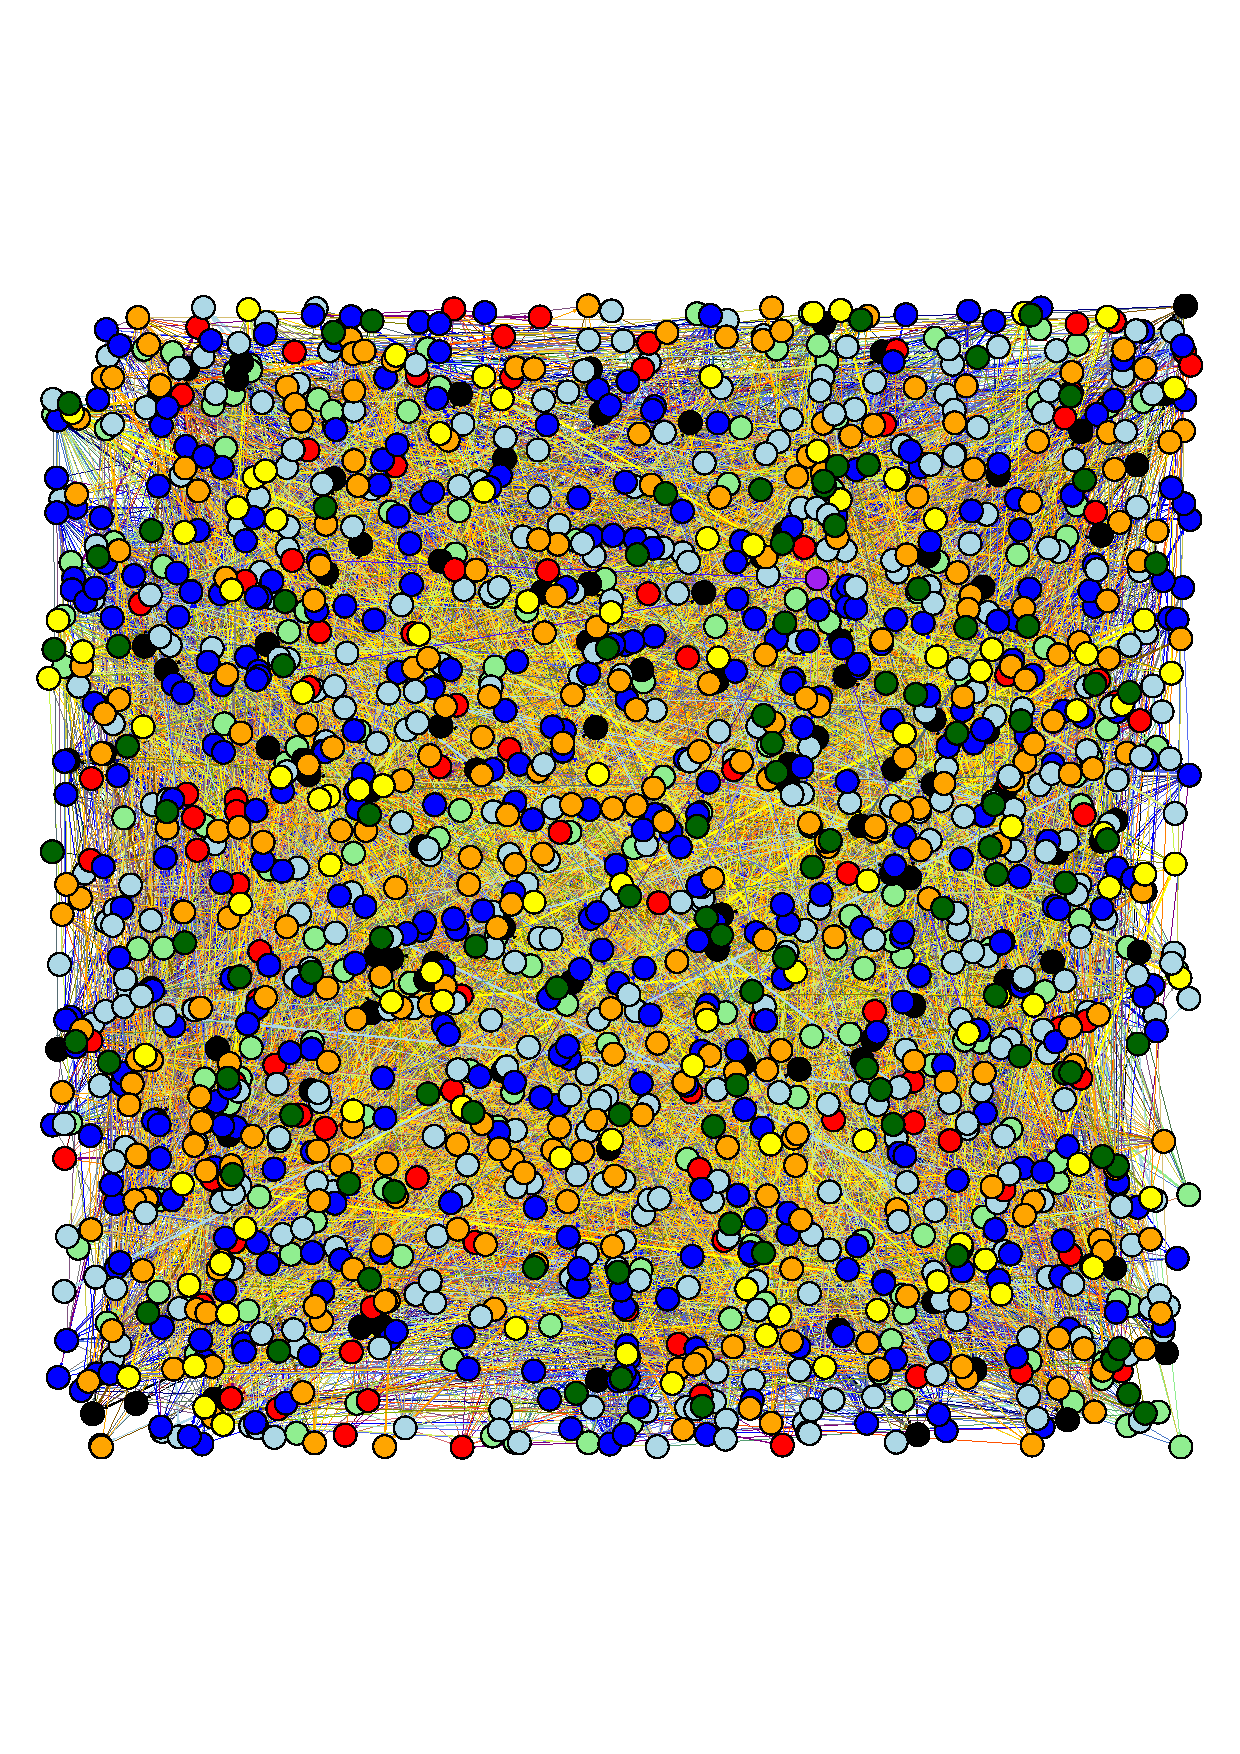
\includegraphics[scale=0.6]{graphbegin.pdf}\caption[Anordnung der Knoten nach dem Einlesen]{Anordnung der Knoten und Kanten direkt nach dem Einlesen in Gephi}\label{graphbegin}
\end{figure}
Für die Berechnung der räumlichen Anordnung der Knoten und Kanten stehen in \textit{Gephi} einige Algorithmen zur Verfügung. Diese berechnen die Anordung der Knoten anhand der Anziehungs- beziehungsweise Abstoßungskraft der Knoten, die aus den relativen Häufigkeiten resultieren. Stärker verbundene Knoten liegen damit näher beieinander als schwach verbundene. Das heißt Knoten, die überhaupt keine Verbindung enthalten, liegen weiter auseinander. Ein Beispiel wäre $Direct\_1$ und $Direct\_3$, da man von der ersten Position nicht direkt zur dritten Position springen kann, sondern zunächst einen Kontaktpunkt an der zweiten Position benötigt. Durch die Anwendung eines Algorithmus ergibt sich somit eine lineare Struktur, die die Positionen aneinander reiht.\\
Für diese Arbeit wurden der Algorithmus \textit{Force Atlas 2} \cite{forceatlas2} und der Algorithmus nach \textit{Yifan Hu} \cite{yifanhu} verwendet, wobei \textit{Yifan Hu} das Netzwerk besser in einzelne Ebenen einteilen kann. Das heißt die Positionen sind hier räumlich deutlicher getrennt. Für die Präsentation der Ergebnisse in Kapitel \ref{resultsnetwork} wurde die räumliche Anordnung der Knoten allerdings noch manuell bearbeitet, um die Ergebnisse anschaulicher zu machen.\\
Das Netzwerk kann in \textit{Gephi} interaktiv bearbeitet werden. Die Daten sowie das Programm sind im elektronischen Anhang enthalten und werden in Kapitel \ref{anhang} näher beschrieben.




\section{Ergebnisse}\label{ergebnisse}

\subsection{Zeitdiskretes Survival-Modell}

Die in diesem Kapitel präsentierten Ergebnisse basieren jeweils auf der bestmöglichen Anzahl an Iterationen. Diese wurden mittels $5$-facher Kreuzvalidierung ermittelt und sind in Abbildung \ref{best_iter} dargestellt. Auf der $x$-Achse ist die Position von $1$ bis $25$ aufgetragen und auf der $y$-Achse die Optimale Iterationsanzahl, die durch $n.trees = 3000$ nach oben begrenzt ist. Es ist zu erkennen, dass für die Positionen $1$ bis $4$ über $2500$ Stümpfe für die Ergebnisse verwendet werden. Dann fällt die Kurve sehr schnell ab bis sie sich bei ungefähr $500$ Iterationen einpendelt. Dieser Abfall ist dadurch zu erklären, dass mit steigender Position die Datenmenge sinkt.
\begin{figure}[H]
	\centering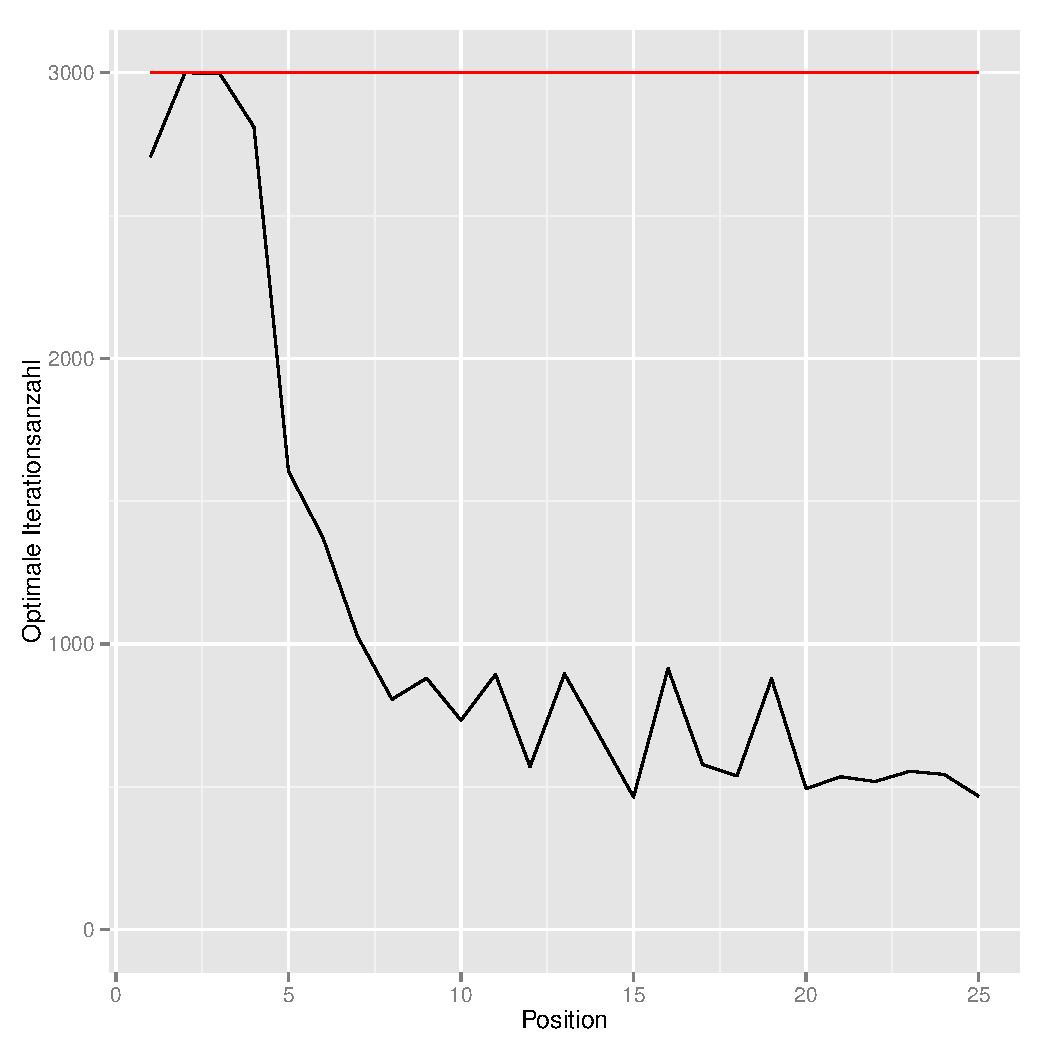
\includegraphics[scale=0.5]{bestIter.pdf}\caption[Optimale Iterationsanzahl]{Optimale Iterationsanzahl des Stochastic Gradient Boosting}\label{best_iter}
\end{figure}
Der relative Einfluss der Features gibt dessen Wichtigkeit bei der Erstellung der Prädiktorfunktion an und ist in Abbildung \ref{variable_importance} dargestellt. Auf der $x$-Achse ist erneut die Position aufgetragen und auf der $y$-Achse der relative Einfluss. Der relative Einfluss aller Features an einer Position ergibt summiert jeweils $100$ und die Balken sind der Größe nach geordnet, das heißt die wichtigsten Variablen sind unten abgebildet. Die Farben der Balken werden in der Legende rechts neben der Abbildung erläutert.\\
An Position $1$ sind nur drei Features vorhanden, wobei $Campaign$, das heißt die Art des Kontaktpunktes, für circa $90 \%$ der Minimierung der Verlustfunktion verantwortlich ist. Die Variablen $Hour$ und $Weekday$ haben kaum Einfluss. An Position $2$ ist die Kampagne immer noch das stärkste Feature, wobei hier auch die Kampagne des ersten Kontaktpunktes und die Zeit, die seit dem ersten Kontaktpunkt vergangen ist, Einfluss haben.\\
\begin{figure}[H]
	\centering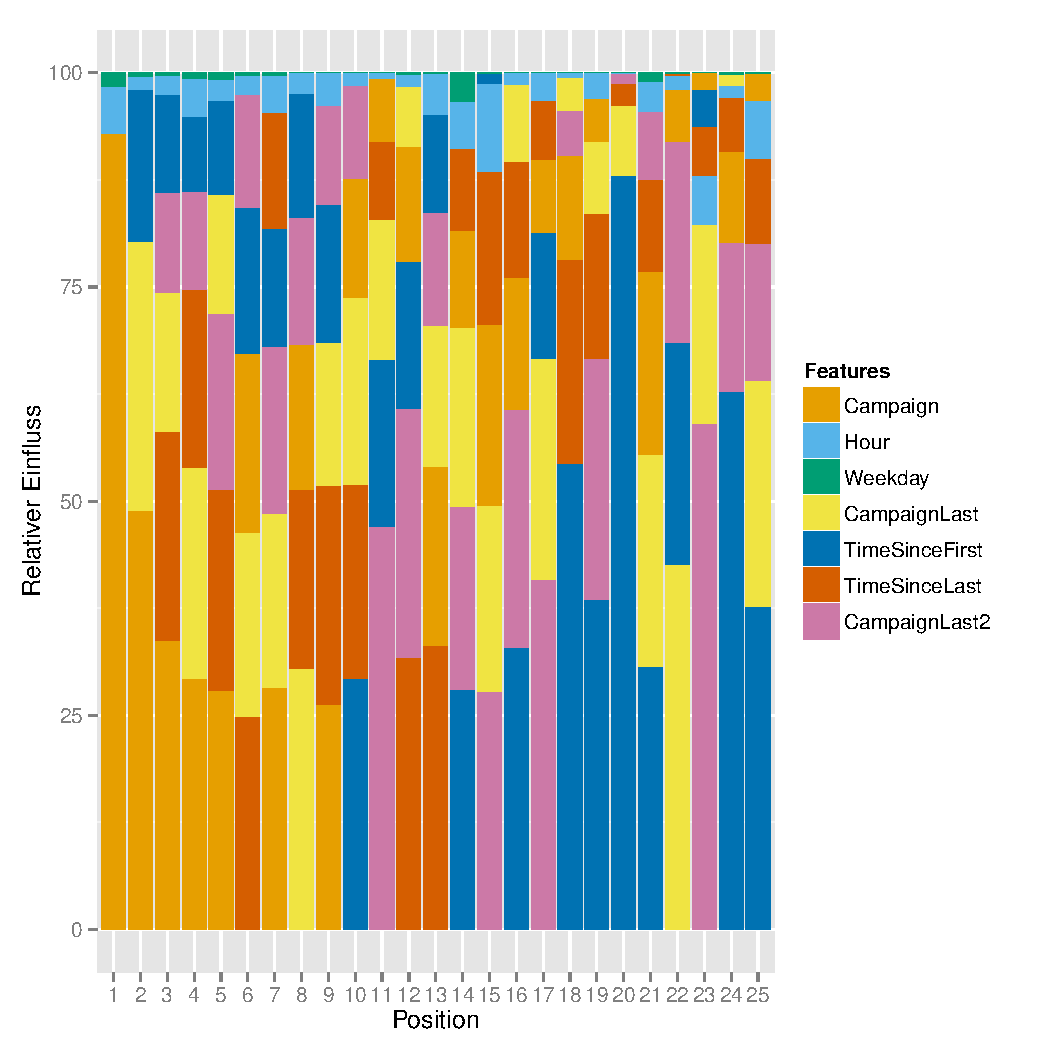
\includegraphics[scale=0.9]{variableImportance.pdf}\caption{Wichtigkeit der Variablen}\label{variable_importance}
\end{figure}
An den Positionen $8$ und $22$ hat die Kampagne des letzten Kontaktpunktes den stärksten Einfluss und damit selbstverständlich auch einen höheren Einfluss als die Kampagne des aktuellen Kontaktpunktes, die insbesondere an den höheren Positionen oft nur noch einen geringen Einfluss hat. Mit steigender Position wird auch die Kampagne des vorletzten Kontaktes wichtiger und ist manchmal das wichtigste Feature. Die Zeit, die seit dem vorherigen Kontaktpunkt vergangen ist, ist bereits an Position $3$ zweitwichtigstes Feature und spielt auch für die folgenden Positionen eine Rolle. Später nimmt die Wichtigkeit dieses Features allerdings ab und die Zeit, die seit dem ersten Kontaktpunkt vergangen ist, wird bedeutend wichtiger. Die Features $Hour$ und $Weekday$ spielen positionsübergreifend kaum eine Rolle.\\
Nachdem die Wichtigkeit der Variablen für die Klassifizierung in konvertierte und nicht-konvertierte Funnel präsentiert wurde, ist nun die Art dieses Einflusses interessant. Dieser wird im folgenden für einige Positionen dargestellt, wobei die Variablen dafür nach positionsspezifischer Wichtigkeit ausgesucht werden und das Augenmerk vor allem auf die niedrigeren Positionen fällt, da dort mehr Daten vorhanden sind. Folglich werden die Features $Hour$ und $Weekday$ garnicht präsentiert, das sie kaum einen Einfluss haben. Die Kampagne des vorletzten Kontaktpunktes $CampaignLast2$ wird an dieser Stelle ebenfalls nicht berücksichtigt, da die Ergebnisse für $Campaign$ beziehungsweise $CampaignLast$ oft sehr ähnlich sind. Im elektronischen Anhang sind die marginalen Effekte aller Features für jeweils jede Position zu finden.\\
In Abbildung \ref{marg_eff_campaign} sind die marginalen Effekte der Variable \textit{Campaign} für die Positionen eins bis vier, von links oben nach rechts unten, aufgetragen. \textit{Campaign} ist an den ersten vier Positionen das wichtigste Feature. Mit steigender Position verliert die Variable deutlich an Einfluss. Auf der $x$-Achse ist die Art des aktuellen Kontaktpunnktes aufgetragen und auf der $y$-Achse der Marginale Effekt.\\
An Position eins haben die Kampagnen \textit{Affiliate - Rest}, \textit{E-Mailing} und \textit{SEM - Brand} im Vergleich zu den restlichen Kampagnen einen starken, positiven Einfluss auf die Konvertierungswahrscheinlichkeit.\\
Das heißt das Bereitstellen von Zinsvergleichen, welche das Zinsangebot der Interhyp AG mit deren Wettbewerbern im Vergleich darstellt, durch die Partner unter \textit{Affiliate - Rest} scheint oft an Position $1$ bereits zur Konvertierung zu führen. Die Partner unter \textit{Affiliate - Partnerprogramm}, die hauptsächlich Rechner der Interhyp AG auf ihren Seiten einbinden, teilweise aber auch Banner schalten oder Verlinkungen in Texten unterbringen, haben an Position $1$ einen deutlich geringeren Effekt. \textit{E-Mailing} sind Mails, die an Interessenten, die schon einen Antrag gestellt haben oder ein Infopaket angefordert hatten, versendet werden. Da dieses Klientel sich offentsichtlich bereits intensiv mit einer Baufinanzierung beschäftigt hat, macht es Sinn, dass diese Mails schon nach wenigen Kontakten häufig zu einer Konvertierung führen und dieser Effekt für spätere Positionen schwächer ist. SEM sind bezahlte Suchergebnisse, hauptsächlich auf Google. \textit{SEM - Brand} bedeutet, dass der Suchbegriff das Wort \textit{Interhyp} enthielt. Dieser Effekt ist deutlich größer als für \textit{SEM - Generisch} beziehungsweise \textit{SEM - Remarketing}, wobei ersteres bedeutet, dass etwas wie \textit{Baufinanzierung} gesucht wurde und zweiteres, dass der potentielle Kunde bereits zuvor auf der Seite von Interhyp war und deshalb nochmal eine Einblendung mit Werbung der Interhyp AG bekommen hat.\\
An Position $2$ stechen neben \textit{Affiliate - Rest}, \textit{SEM - Brand} und \textit{E-Mailing} auch \textit{Direct} und \textit{Generic} durch ihre Marginalen Effekte leicht hervor. \textit{Direct} bedeutet, dass jemand im Browser direkt \textit{www.interhyp.de} eingegeben hat und \textit{Generic}, dass jemand über einen unbezahlten Link zur Interhyp kam.
Für die Positionen $3$ und $4$ ist vor allem \textit{Generic} wichtig. \textit{Display}, \textit{Social Media}, \textit{SEO} sowie die Kooperationen spielen, neben den bereits erwähnten, keine große Rolle für die ersten vier Positionen.
\begin{figure}[H]
	\centering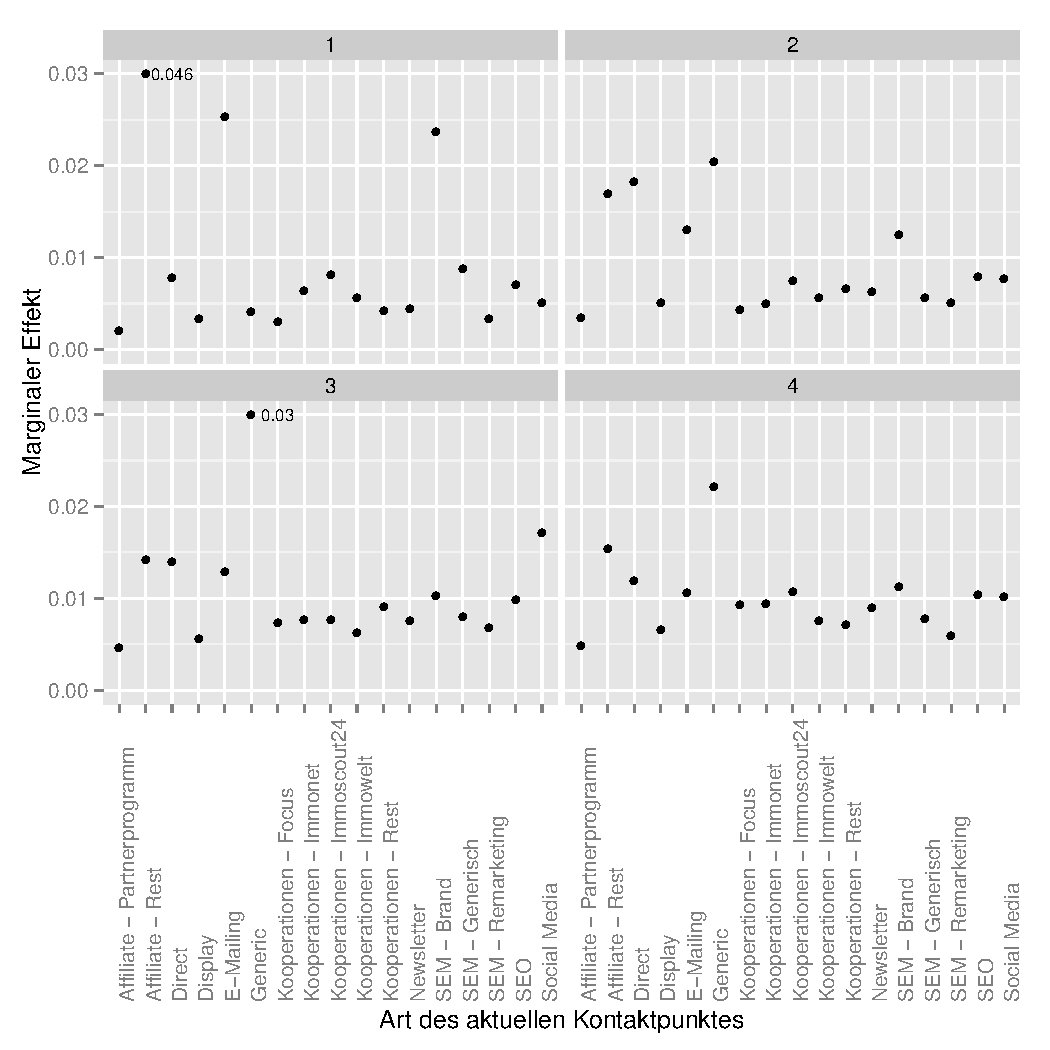
\includegraphics[scale=0.75]{marg_eff_campaign.pdf}\caption[Marginaler Effekt von \textit{Campaign}]{Marginaler Effekt des Features \textit{Campaign} an den Positionen $1$, $2$, $3$ und $4$}\label{marg_eff_campaign}
\end{figure}
An den Positionen $4$, $6$ und $7$ ist \textit{CampaignLast} das zweitwichtigste Feature sowie an Position $8$ das wichtigste. Dessen marginalen Effekte sind in Abbildung \ref{marg_eff_campaignLast} dargestellt. Hier heben sich teilweise die selben Kategorien hervor, wobei die Unterschiede zwischen den Kampagnen kleiner sind. Überraschend ist, dass hier auch \textit{Social Media} einen starken Effekt hat. Allerdings liegen hierfür kaum Daten vor, wie in Abbildung \ref{campaign} zu erkennen ist.\\
\begin{figure}[H]
	\centering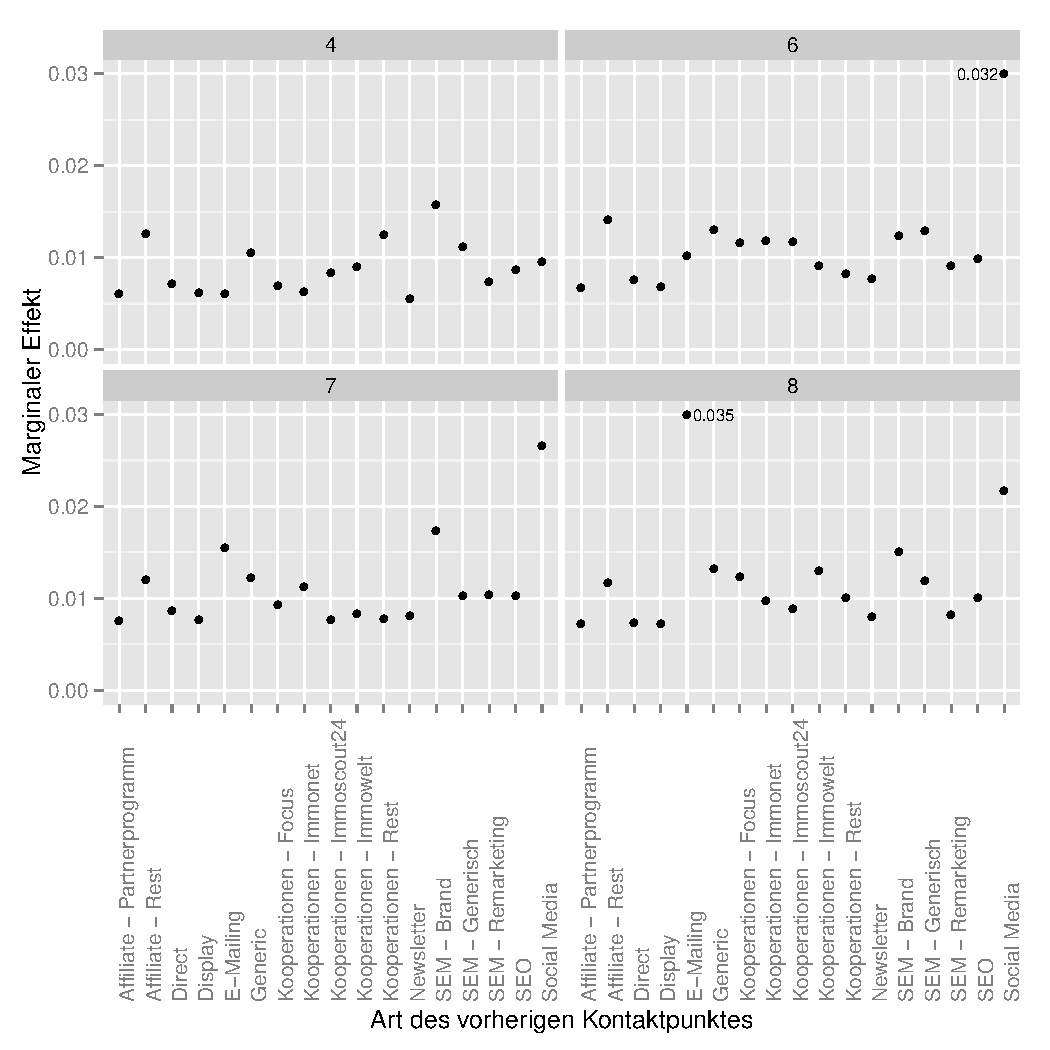
\includegraphics[scale=0.75]{marg_eff_campaignLast.pdf}\caption[Marginaler Effekt von \textit{CampaignLast}]{Marginaler Effekt des Features \textit{CampaignLast} an den Positionen $4$, $6$, $7$ und $8$}\label{marg_eff_campaignLast}
\end{figure}
Das Feature \textit{TimeSinceFirst} ist an den Positionen $10$ und $14$ das wichtigste sowie an Position $11$ und $12$ das zweit- beziehungsweise drittwichtigste. \textit{TimeSinceLast} ist an den Positionen $6$, $12$ und $13$ das wichtigste Feature und an Position $8$ das zweitwichtigste Feature. Die marginalen Effekte für diese Positionen sind in Abbilung \ref{marg_eff_time} dargestellt, wobei diese an anderen Positionen ähnlich aussehen. Auf der $x$-Achse ist die Zeit in Tagen aufgetragen und auf der $y$-Achse die Marginalen Effekte. Für beide Features und alle Positionen steigen die marginalen Effekte mit der Zeit, wobei der Effekt bei \textit{TimeSinceLast} etwas größer ist.\\
Dass die Konvertierungswahrscheinlichkeit bei zeitlich längeren Funnels höher ist, könnte man dadurch erklären, dass die Entscheidung für den Bau eines Hauses oder ähnlichem und das damit verbundene Ausfüllen eines Online-Antrages viel Zeit in Anspruch nimmt. Dass für die Zeit seit des vorherigen Kontaktes der selbe Effekt auftritt, könnte man ähnlich erklären. Bei der Entscheidung für eine Baufinanzierung sind viele Dinge zu beachten. So erscheint es plausibel, dass sich interessierte Kunden eine längere Zeit auch offline mit dem Thema beschäftigen und später wieder online den Kontakt zur Interhyp AG suchen.
\begin{figure}[H]
	\centering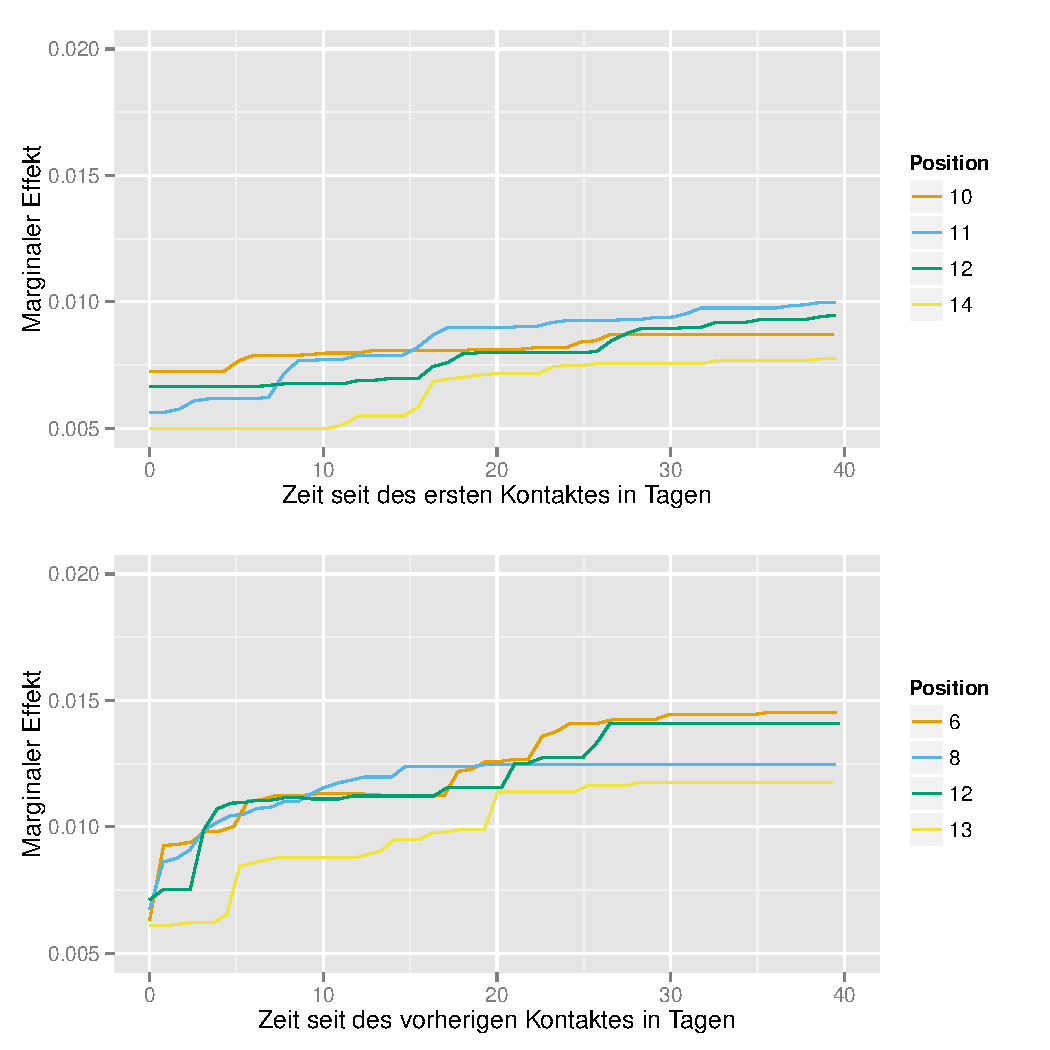
\includegraphics[scale=0.75]{marg_eff_time.pdf}\caption[Marginaler Effekt von \textit{TimeSinceFirst} und \textit{TimeSinceLast}]{Marginaler Effekt des Features \textit{TimeSinceFirst} an den Positionen $10$, $11$, $12$ und $14$ (oben) und des Features \textit{TimeSinceLast} an den Positionen $6$, $8$, $12$ und $13$ (unten)}\label{marg_eff_time}
\end{figure}
Bis hierhin wurden die Ergebnisse des, auf den Trainingsdaten geschätzten, Modells vorgestellt. Nun soll das Modell auf die Testdaten angewendet werden, um die Prognosegüte zu beurteilen.\\
Wenn man die geschätzte Prognosefunktion auf die Testdaten anwendet, bekommt man für jede Position und jede ID aus den Testdaten die Hazardrate, das heißt die Wahrscheinlichkeit an einer bestimmten Position zu konvertieren. Diese sind sowohl für konvertierte als auch nicht-konvertierte Funnels sehr niedrig, da die absolute Anzahl an nicht-konvertierten Funnels deutlich überwiegt. Um die Prognosegüte des Modells näher zu betrachten wurde deshalb für jede Position eine ROC-Kurve berechnet. Diese sind in Abbildung \ref{roc} für vier Positionen beispielhaft dargestellt.\\
%An Position $1$ ist dieser Unterschied noch nicht sehr deutlich. Dies kann daran liegen, dass hier nur die Features \textit{Campaign}, \textit{Hour} und \textit{Weekday} einfließen und noch keine Informationen über vorherige Positionen vorliegen. Von dort steigen die Hazardraten an, wobei dieser Anstieg in den konvertierten Funnels deutlich stärker ist als in den nicht-konvertierten. Ab Position $6$ werden die Konvertierungswahrscheinlichkeiten wieder geringer, wobei immer noch ein deutlicher Unterschied zwischen konvertiert und nicht-konvertiert zu erkennen ist.\\
Auf der $x$-Achse ist der Anteil der nicht-konvertierten Funnels, die als konvertiert vorhergesagt wurden aufgetragen und auf der $y$-Achse der Anteil der konvertierten Funnels, die auch als konvertiert vorhergesagt wurden. Je weiter die ROC-Kurve also oberhalb der roten Diagonalen liegt, desto besser kann das Modell zwischen konvertierten und nicht-konvertierten Funnels trennen. Für Position $3$ liegt die Kurve für alle Punkte überhalb der Kurve von Position $1$. Dies ist dadurch zu erklären, dass an Position $3$ mehr Informationen zur Erstellung des Modells verwendet werden als an Position $1$. Für Position $15$ und $22$ ist das Modell schlechter als an Position $3$. Die Kurven für die späteren Positionen sind deutlich rauher. Dies ist darauf zurück zu führen, dass dort weniger Datenpunkte vorhanden sind. Durch das Einbringen des Offsets kann die Prognoseleistung des Modells allerdings halbwegs konstant gehalten werden.\\
\begin{figure}[H]
	\centering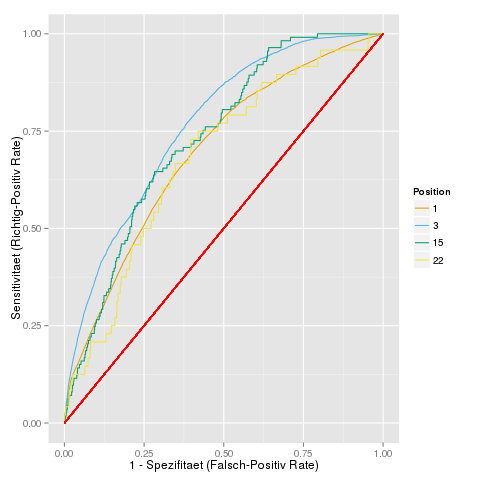
\includegraphics[scale=0.5]{roc.png}\caption[ROC-Kurve]{ROC-Kurve für die Positionen $1$, $3$, $15$ und $22$}\label{roc}
\end{figure}
Dies ist in Abbildung \ref{auc} noch deutlicher zu erkennen. Hier ist die Fläche unterhalb der ROC-Kurve (AUC) für jede Position abgebildet. Dieser Wert fällt zwischen Position $15$ und $22$ unter $0.75$ ab, hält sich ansonsten aber relativ konstant auf $0.75$. Das heißt die Wahrscheinlichkeit, dass bei einer konvertierten Beobachtung die Hazardrate größer ist als bei einer nicht-konvertierten Beobachtung ist positionsübergreifend circa $0.75$.
\begin{figure}[H]
	\centering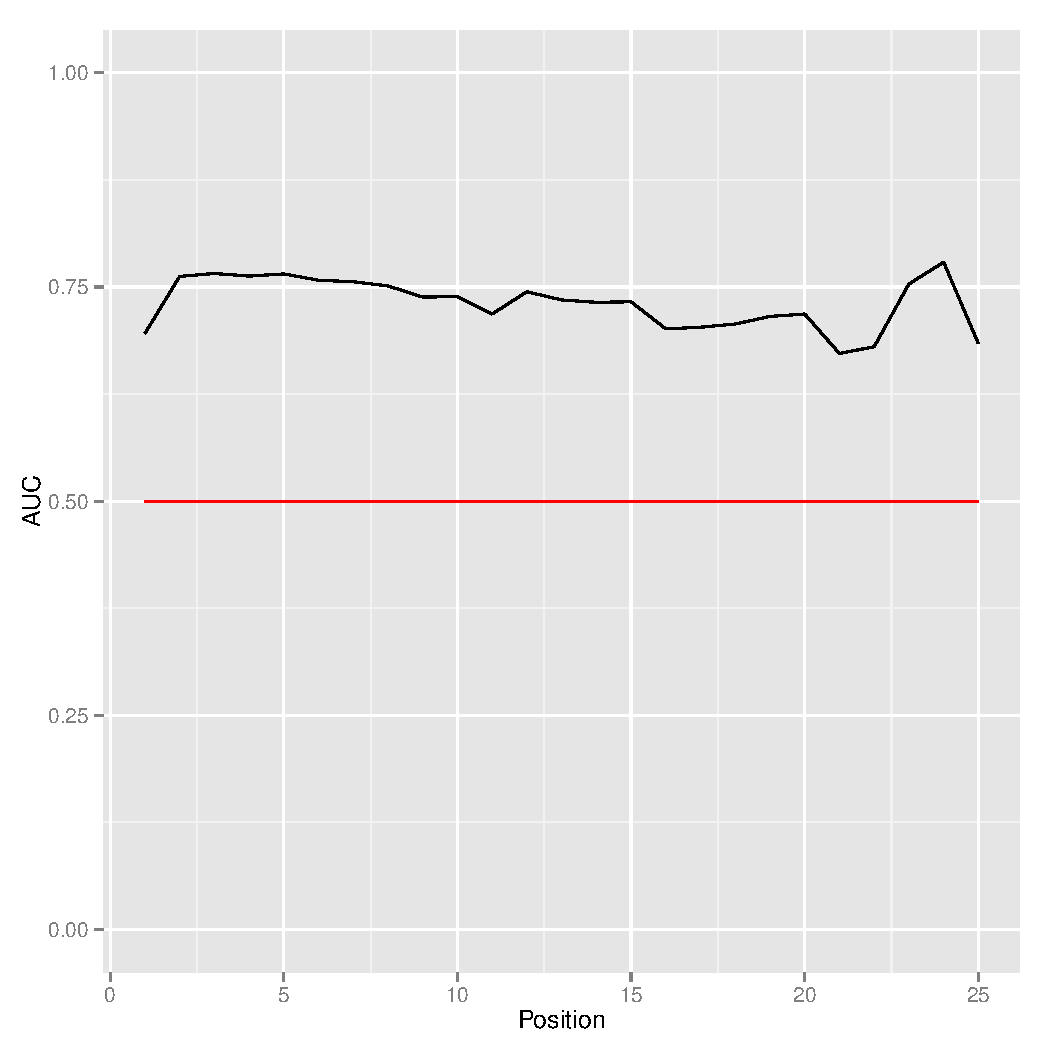
\includegraphics[scale=0.75]{auc.pdf}\caption[AUC-Wert]{AUC für alle Positionen}\label{auc}
\end{figure}

\subsection{Sequential Pattern Mining}\label{ergspm}

Der in Kapitel \ref{spm} beschriebene Algorithmus wurde zunächst seperat auf alle konvertierten sowie nicht-konvertierten Funnels angewendet. Dabei wurden Funnels mit der Länge eins ausgeschlossen, da in diesen offentsichtlich keine interessanten Sequenzen enthalten sein können. Der minimale Support wurde auf $0.05$ gesetzt, so dass nur Sequenzen, die in mindestens $5 \%$ aller Funnels vorkommen, als Ergebnis ausgegeben werden. In Abbildung \ref{spm_all} sind diese Sequenzen geplottet, wobei auf der $x$-Achse der Suppport aufgetragen ist und die Sequenzen anhand des Supports der Sequenzen in den konvertierten Funnels absteigend geordnet sind. An den Stellen, wo keine Balken geplottet sind, war der Support kleiner als $0.05$. Die Namen der Kampagnen sind teilweise abgekürzt, um die Darstellung zu verbessern. \textit{AffPar} steht für \textit{Affiliate - Partnerprogramm}, \textit{Dir} für \textit{Direct} und \textit{Dis} für \textit{Display}. Außerdem ist zu beachten, dass die Sequenzen nicht exakt in der dargestellten Weise in den Funnels vorkommen müssen, sondern auch Abstände zwischen den aufeinanderfolgenden Kampagnen erlaubt sind.\\
Der Support von Sequenzen der Länge eins, wie \textit{<\{Dir\}>} oder \textit{<\{SEO\}>}, geben lediglich an, wie groß der Anteil der Funnels ist, die diese Kampagne mindestens einmal enthalten. Interessanter sind Sequenzen, die mindestens zwei Kampagnen enthalten. Hier fällt auf, dass Sequenzen mit wiederholtem \textit{Direct}-Kontakt in den konvertierten Funnels stärker sind. Umgekehrt sind  Sequenzen mit wiederholtem \textit{Affiliate - Partnerprogramm}-Kontakt in den nicht-konvertierten Funnels stärker. Allerdings haben die Sequenzen insgesamt einen sehr geringen Support. Das liegt vor allem daran, dass die Daten zu großem Teil aus sehr kurzen Funnels bestehen (siehe Abbildung \ref{funnelLength}).\\
\begin{figure}[H]
	\centering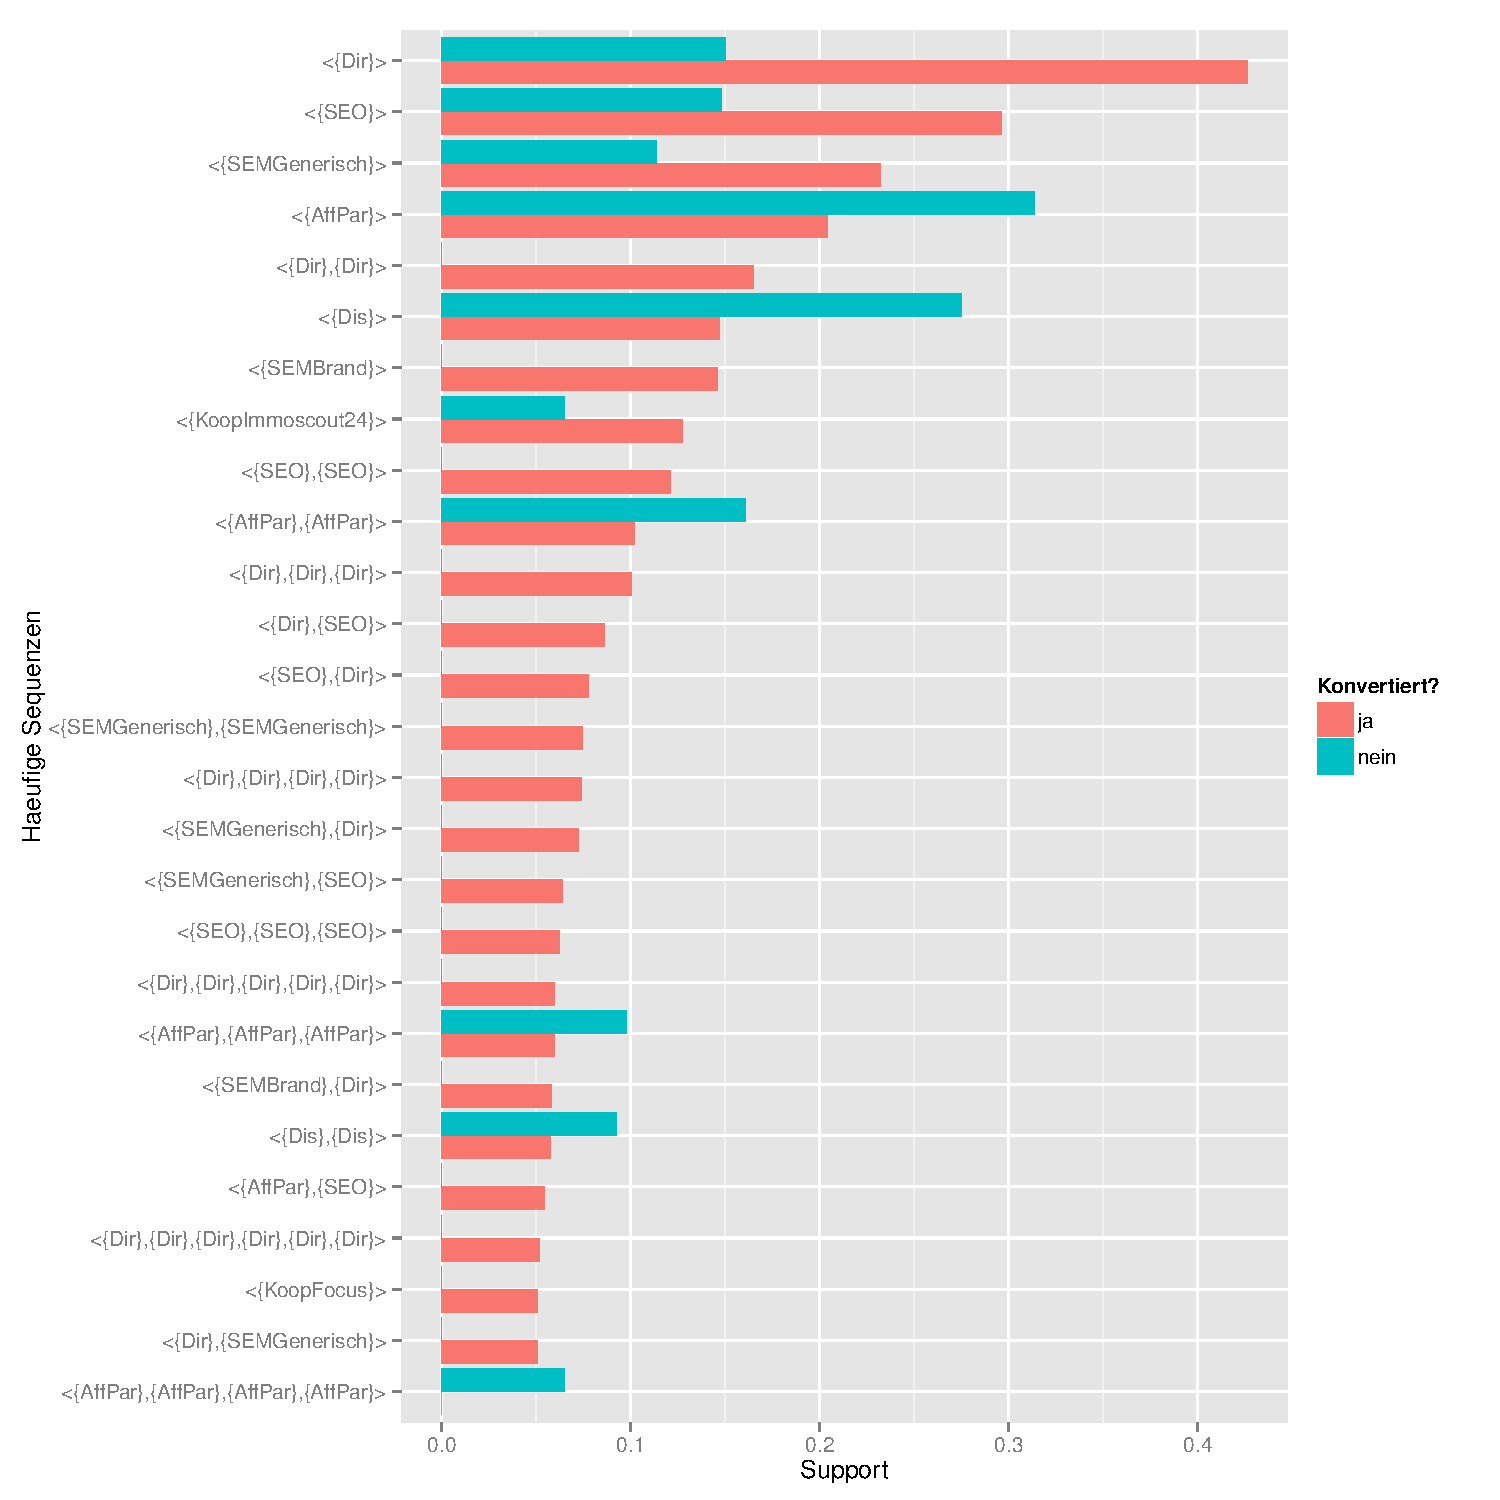
\includegraphics[scale=0.6]{spm_all.pdf}\caption[Häufige Sequenzen]{Häufige Sequenzen in den konvertierten und nicht-konvertierten Funnels}\label{spm_all}
\end{figure}
Deshalb wurde der SPADE-Algorithmus erneut seperat auf konvertierte und nicht-konvertierte Funnel angewendet, wobei dieses mal nur Funnels verwendet wurden, die eine Mindestlänge von $15$ haben. Der minimale Support wurde auf $0.2$ erhöht, um die Anzahl an häufigen Sequenzen zu beschränken. Die Ergebnisse sind in Abbildung \ref{spm_min15} dargestellt.\\
\begin{figure}[H]
	\centering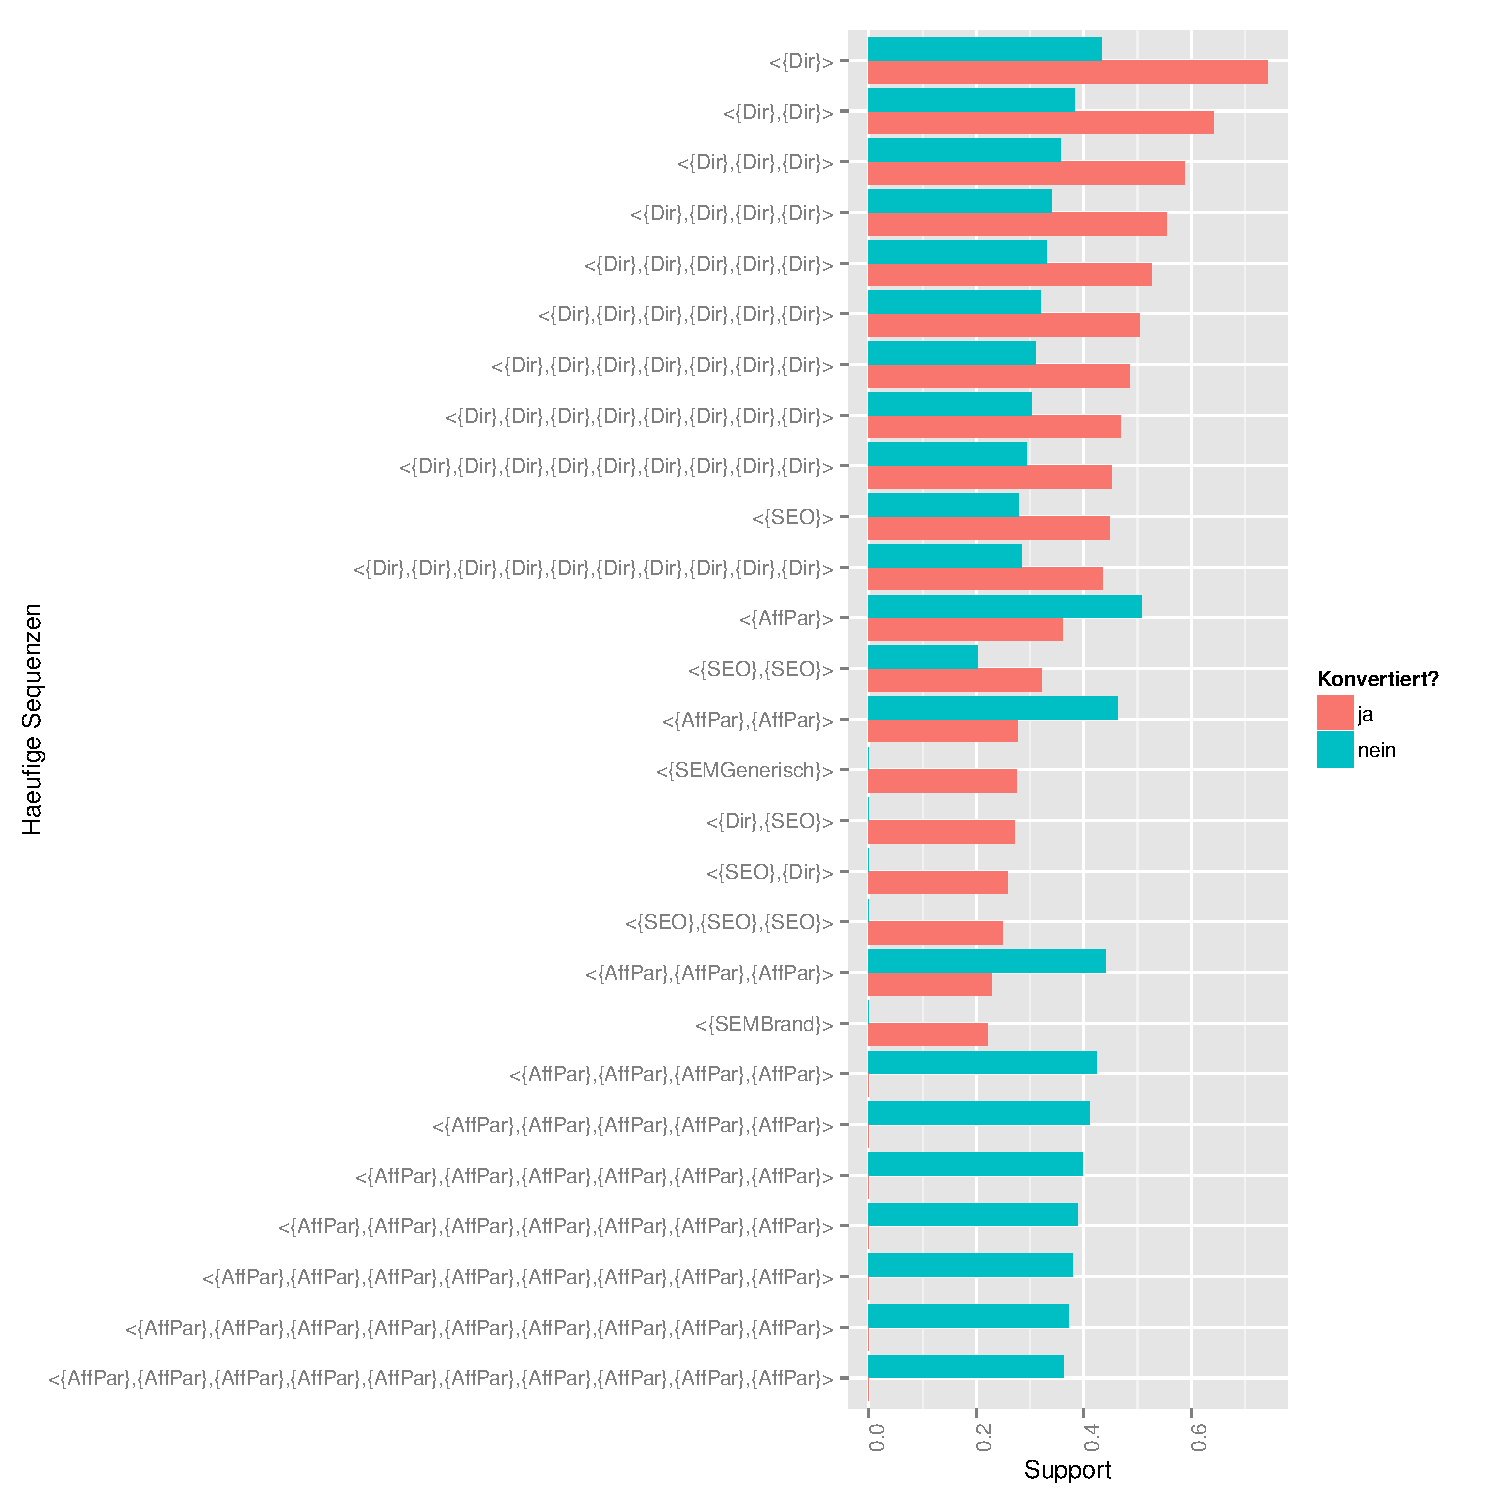
\includegraphics[scale=0.6]{spm_min15.pdf}\caption[Häufige Sequenzen in Funnels mit mindestens $15$ Kontaktpunkten]{Häufige Sequenzen in den konvertierten und nicht-konvertierten Funnels mit mindestens $15$ Kontakten}\label{spm_min15}
\end{figure}
Die Sequenzen haben jetzt teilweise einen Support, der größer als $0.5$ ist, das heißt mehr als die Hälfte der Funnels beinhalten diese Sequenz. Hier ist noch deutlicher zu erkennen, dass die \textit{Direct}-Sequenzen in den konvertierten Funnels stärker sind als in den nicht-konvertierten Funnels. Die \textit{Affiliate - Partnerprogramm}-Sequenzen haben in den nicht-konvertierten Funnels einen Support von ungefähr $40 \%$ und in den konvertierten Funnels einen Support von unter $20 \%$.\\

\subsection{Netzwerk}\label{resultsnetwork}

Mit dem Programm \textit{Gephi} ist es möglich interaktiv mit dem Netzwerk zu arbeiten. Eine komplette Analyse des Netzwerkes würde den Rahmen dieses Berichtes sprengen. Deshalb soll hier nur beispielhaft, anhand einiger Grafiken, dargestellt werden, welche Ergebnisse man aus dem Netzwerk ziehen kann. Dafür wurde ein Ausschnitt an Position $2$ gewählt. Eine genauere Anleitung zur Verwendung von \textit{Gephi} ist zudem in Kapitel \ref{anhang} zu finden.

\subsubsection*{Relative Ausgänge}

Zunächst werden die relativen Ausgänge präsentiert, das heißt die Gewichte aller Kanten, die einen Knoten verlassen, ergeben in der Summe $1$.\\
Abbildung \ref{out_labels} enthält den Ausschnitt des Netzwerkes an Position $2$ mit den relativen Ausgängen. Die Knoten sind farblich codiert und mit Labels versehen. Am rechten Bildrand ist noch eine Kampagne der ersten Position \textit{SEO\_1} zu erkennen. Von dort und den anderen Kampagnen der ersten Position führen die Kanten zu den Kampagnen der zweiten Position in der Mitte der Abbildung. Für Funnels, die mehr als zwei Kontaktpunkte haben gehen die Kanten von diesen Kampagnen zu den Knoten der dritten Positionen jenseits des linken Bildrandes. Die Kampagne \textit{Affiliate - Partnerprogramm\_3} ist noch zu erkennen.\\
Funnels, die lediglich über zwei Kontaktpunkte verfügen, enden in \textit{Fail\_2} im Falle einer Nicht-Konvertierung beziehungsweise in \textit{Success\_2} im Falle einer Konvertierung.
\begin{figure}[H]
	\centering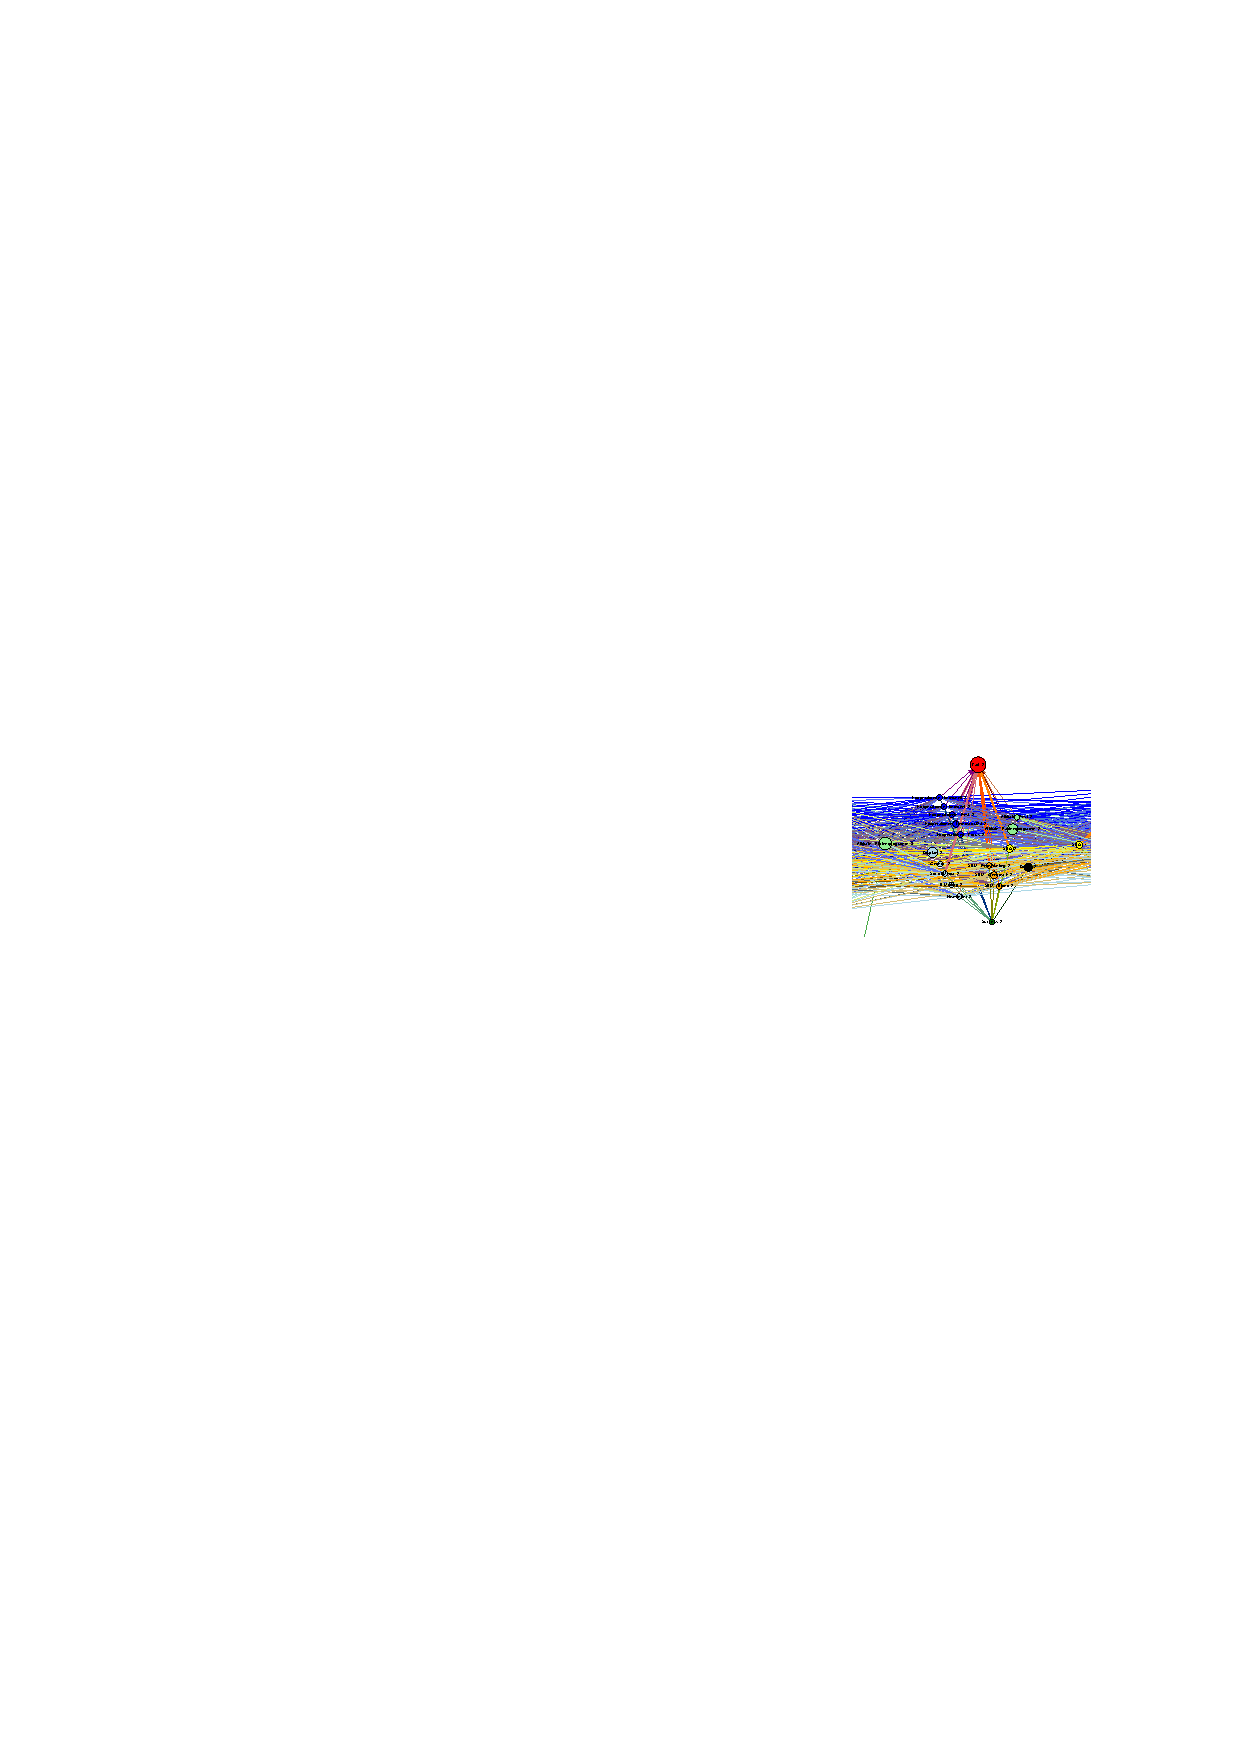
\includegraphics[scale=2.5]{out_labels.pdf}\caption[Relative Ausgänge]{Auschnitt des Netzwerkes an Position $2$ mit relativen Ausgängen}\label{out_labels}
\end{figure}
Die Dicke der Kanten hängt von deren Gewichtung ab. Abbildung \ref{out_filter_2_succ} enthält den selben Ausschnitt, wobei nun ein Filter von $0.02$ auf die Kanten angewendet wurde. Somit sind nur noch Kanten abgebildet, deren Gewicht größer als $0.02$ ist. Durch das Auswählen des Knoten \textit{Success\_2} werden alle Knoten hervorgehoben, die nach der Anwendung des Filters noch durch eine Kante mit \textit{Success\_2} verbunden sind.\\
Das heißt über $2 \%$ aller Nutzer, die als zweiten Kontaktpunkt $Direct$ haben, konvertieren an der zweiten Position. Selbiges gilt für \textit{Affiliate - Rest}, \textit{Generic}, \textit{SEM - Brand} und \textit{E-Mailing}. Durch Veränderung der Filter und weiterer Einstellungen können die Ergebnisse auch noch genauer betrachtet werden. Wie bereits erwähnt, ist in Kapitel \ref{anhang} ein Tutorial dazu vorhanden.\\
Interessant ist an dieser Stelle, dass die fünf hervorgehobenen Kampagnen gleichzeitig die fünf stärksten Kampagnen bei den Marginalen Effekten des Features \textit{Campaign} an Position $2$ sind. Das heißt die Ergebnisse des Survival-Modells können durch die Betrachtung des Netzwerkes überprüft und bestätigt werden.
\begin{figure}[H]
	\centering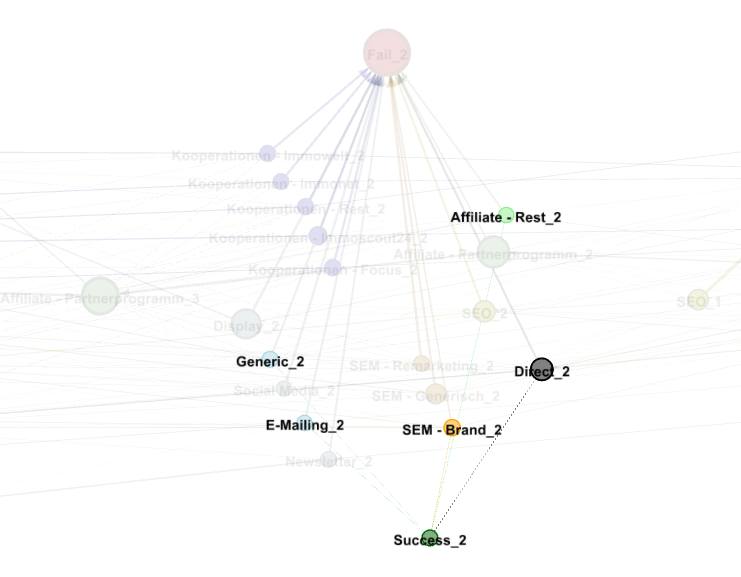
\includegraphics[scale=0.4]{out_filter_2_succ.png}\caption[Relative Ausgänge mit Filter $0.02$]{Auschnitt des Netzwerkes an Position $2$ mit relativen Ausgängen, Filter $0.02$ und Fokus auf den konvertierten Funnels}\label{out_filter_2_succ}
\end{figure}
Abbildung \ref{out_filter_50_fail} enthält erneut den selben Ausschnitt des Netzwerkes, wobei nun ein Filter von $0.5$ angewendet wurde und der Fokus auf den nicht-konvertierten Funnels liegt. Von den hervorgehobenen Knoten enden also jeweils mindestens die Hälfte der Beobachtungen ohne Konvertierung.\\
Analog zu der Betrachtung von \textit{Success\_2} oder \textit{Fail\_2} können auch die Kampagnen durch Auswählen näher betrachtet werden. Durch die positionsübergreifende Betrachtung können zudem die häufigen Sequenzen, die mittels des Sequential-Pattern-Mining Algorithmus ermittelt wurden, erkannt werden.
\begin{figure}[H]
	\centering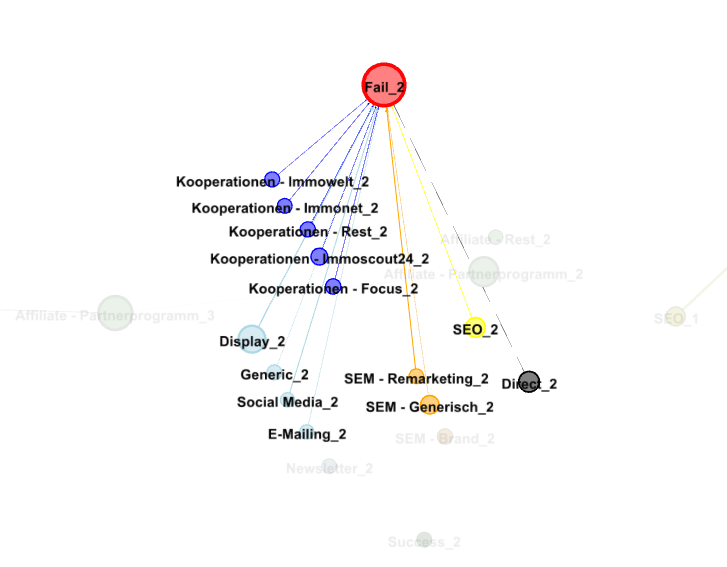
\includegraphics[scale=0.4]{out_filter_50_fail.png}\caption[Relative Ausgänge mit Filter $0.5$]{Auschnitt des Netzwerkes an Position $2$ mit relativen Ausgängen, Filter $0.5$ und Fokus auf den nicht-konvertierten Funnels}\label{out_filter_50_fail}
\end{figure}

\subsubsection*{Relative Eingänge}

In diesem Abschnitt wird erneut Position $2$ betrachtet, wobei die Kanten nun anhand der relativen Eingänge gewichtet sind. Das heißt die Gewichte aller Kanten, die in einen bestimmten Knoten gehen, ergeben aufsummiert $1$. Abbildung \ref{in_labels} enthält den Ausschnitt des Netzwerkes. Am rechten beziehungsweise linken Bildrand ist erneut eine Kampagne von Position $1$ beziehungsweise $3$ zu erkennen. Die Farben und Beschriftungen der Knoten sind die selben wie in Abbildung \ref{out_labels}. 
\begin{figure}[H]
	\centering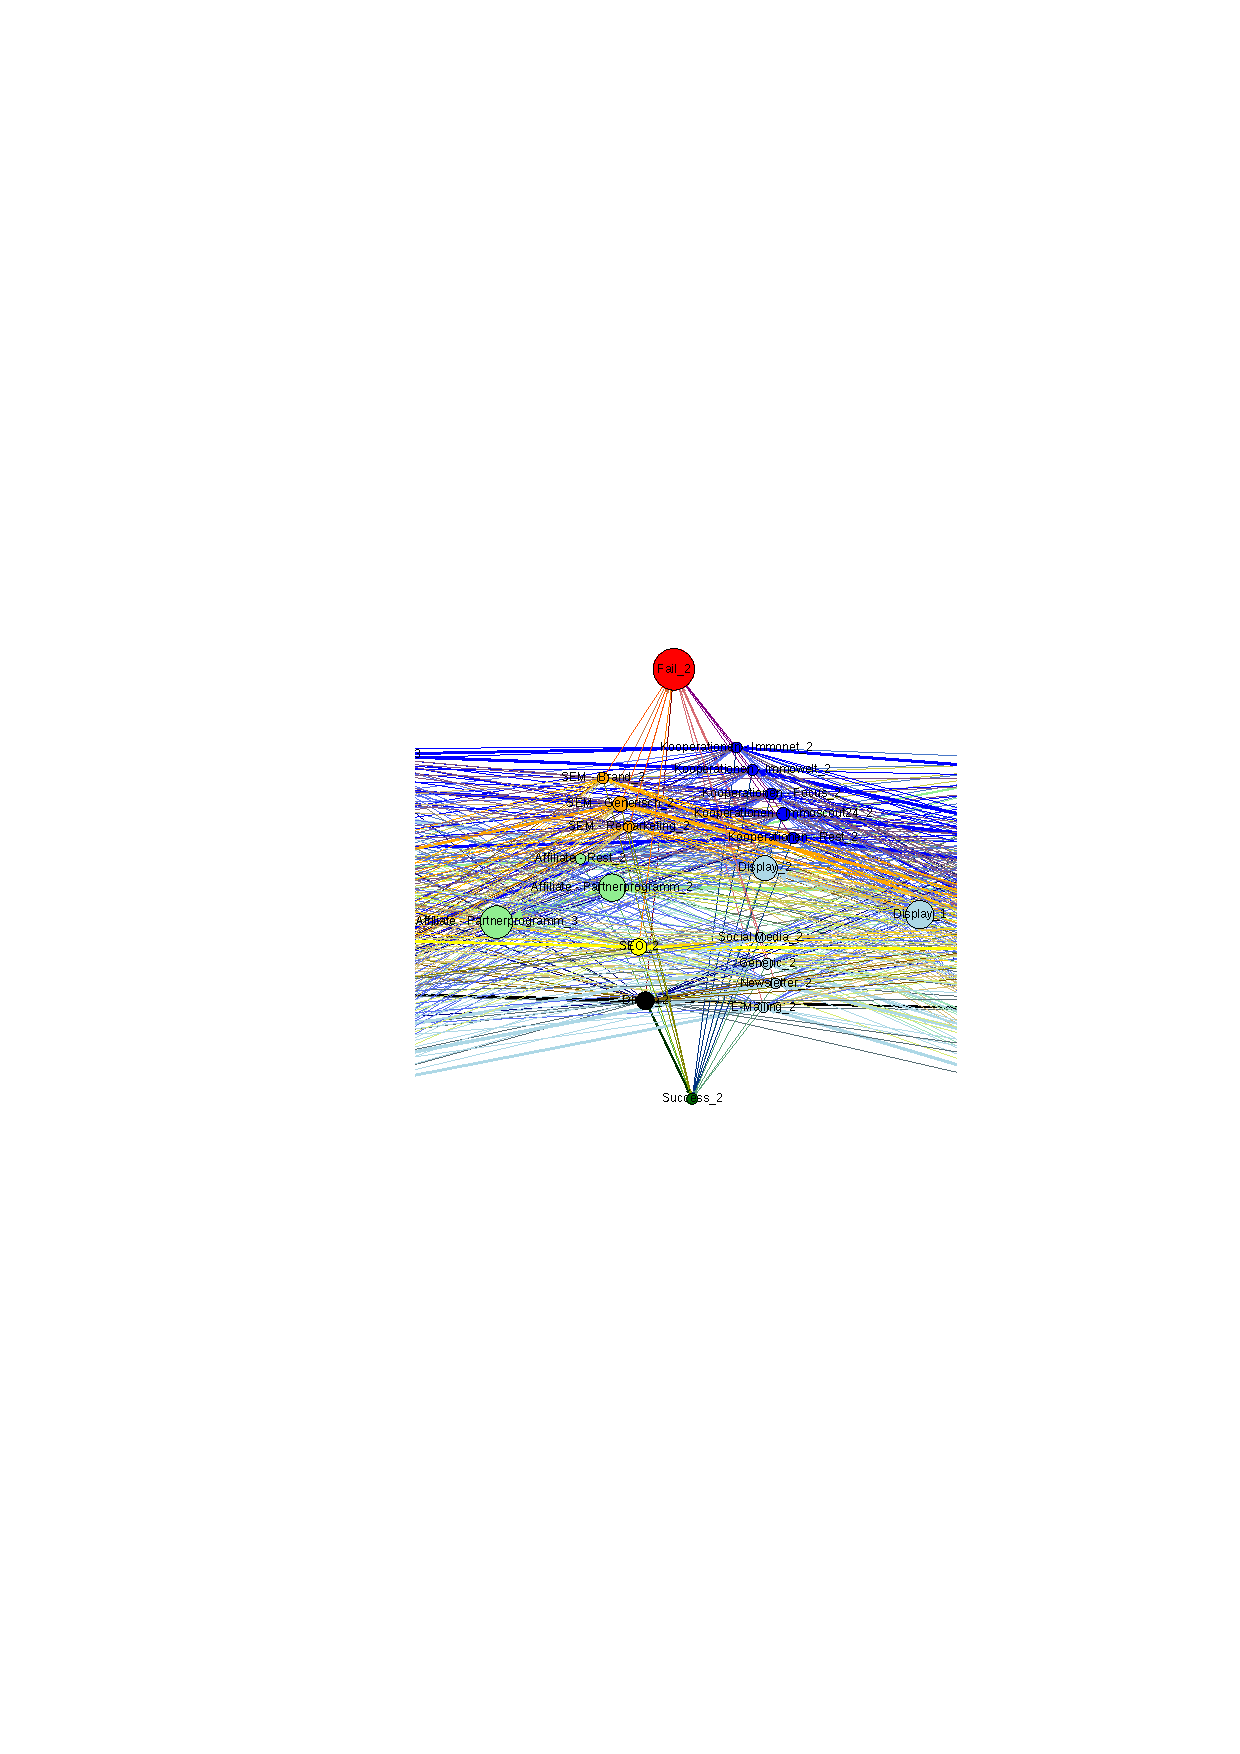
\includegraphics[scale=1]{in_labels.pdf}\caption[Relative Eingänge]{Auschnitt des Netzwerkes an Position $2$ mit relativen Eingängen}\label{in_labels}
\end{figure}
Auf diesen Ausschnitt wurde ein Filter von $0.1$ angewendet, wobei der Fokus auf den konvertierten Funnels liegt (siehe Abbildung \ref{in_filter_10_succ}). Die hervorgehobenen Knoten \textit{SEM-Generisch\_2}, \textit{Display\_2}, \textit{SEO\_2} und \textit{Direct\_2} machen jeweils mehr als $10 \%$ der konvertierten Funnels aus, die aus zwei Kontaktpunkten bestehen. Das heißt hier kann nun betrachtet werden, aus welchen Kampagnen des letzten Kontaktpunktes sich die Menge der konvertierten beziehungsweise nicht-konvertierten Funnels zusammensetzen. Zudem ist es auch möglich eine Kampagne zu markieren, so dass erkennbar wird, aus welchen Kampagnen der vorherigen Position, sich diese zusammensetzt. Im Gegensatz dazu, war die Interpretation im vorherigen Kapitel eine andere. Dort wurde betrachtet, wohin die Nutzer von einem Knoten aus gehen.
\begin{figure}[H]
	\centering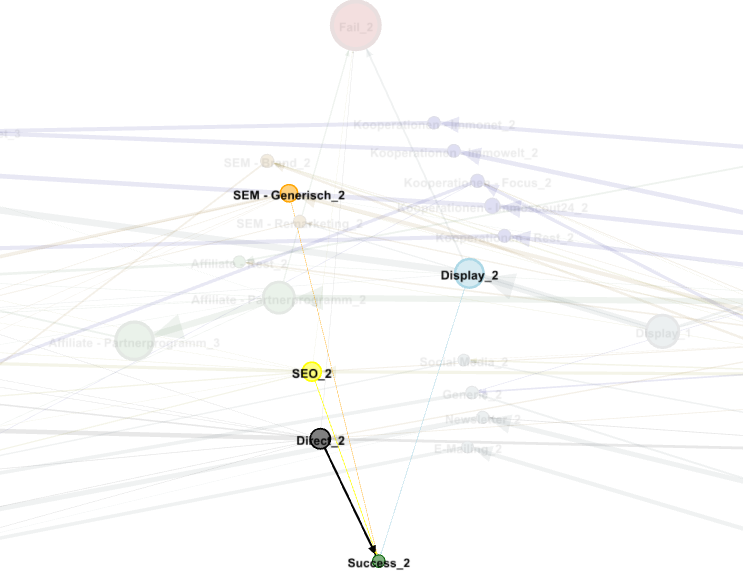
\includegraphics[scale=0.4]{in_filter_10_succ.png}\caption[Relative Eingänge mit Filter $0.1$ und Fokus auf Konvertierten]{Auschnitt des Netzwerkes an Position $2$ mit relativen Eingängen, Filter $0.1$ und Fokus auf den konvertierten Funnels}\label{in_filter_10_succ}
\end{figure}
Abbildung \ref{in_filter_10_fail} enthält den selben Ausschnitt mit dem selben Filter von $0.1$, wobei nun die nicht-konvertierten Funnels betrachtet werden. Das heißt von den Funnels, die nach zwei Kontaktpunkten ohne Konvertierung abbrechen, haben jeweils mindestens $10\%$ als letzten Kontaktpunkt \textit{Affiliate - Partnerprogramm\_2}, \textit{Display\_2}, \textit{SEO\_2} oder \textit{Direct\_2}.
\begin{figure}[H]
	\centering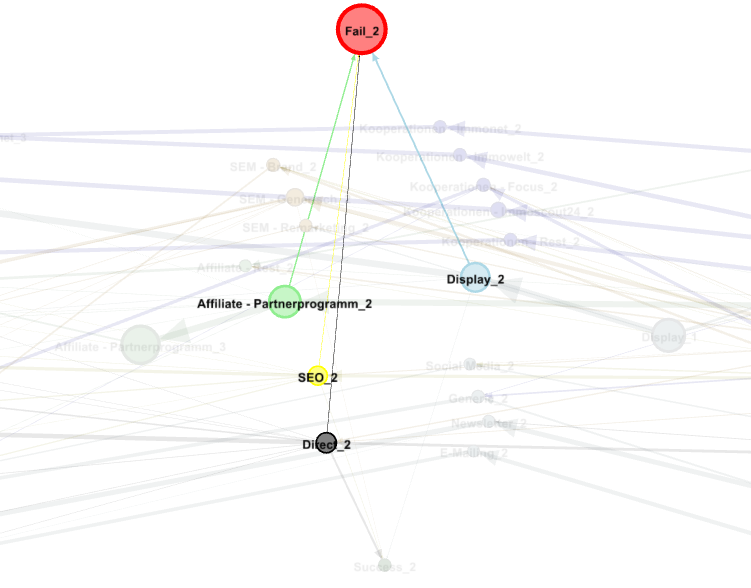
\includegraphics[scale=0.4]{in_filter_10_fail.png}\caption[Relative Eingänge mit Filter $0.1$ und Fokus auf Nicht-Konvertierten]{Auschnitt des Netzwerkes an Position $2$ mit relativen Eingängen, Filter $0.1$ und Fokus auf den nicht-konvertierten Funnels}\label{in_filter_10_fail}
\end{figure}
\section{Zusammenfassung}

\begin{frame}\frametitle{Inhalt}
	\tableofcontents[currentsection,hideallsubsections]
\end{frame}

\begin{frame}\frametitle{Zusammenfassung der Ergebnisse}
	\begin{itemize}
		\item Zeitdiskretes Survival-Modell
		\begin{itemize}
			\item Klassifikation in konvertierte und nicht-konvertierte Funnels
			\item Marginale Effekte der Features
		\end{itemize}
		\item Sequential Pattern Mining
		\item Netzwerk
		\begin{itemize}
			\item Visualisierung der gesamten Daten
			\item Bestätigung der Ergebnisse aus Survival-Modell und Sequential Pattern Mining
			\item Tutorial zum interaktiven Arbeiten im Bericht
		\end{itemize}
	\end{itemize}
\end{frame}

\begin{frame}{Literatur}
	\begin{thebibliography}{1}
		\bibitem{} J. H. Friedman \& B. E. Popescu (2005): {\glqq Predictive Learning via Rule Ensembles\grqq}.
		\bibitem{} R. Agrawal \& R. Srikant (1995): {\glqq Mining sequential patterns\grqq}.
		\bibitem{} M. J. Zaki (2001): {\glqq SPADE: An efficient algorithm for mining frequent sequences\grqq}.
		\bibitem{} M. Bastian, S. Heymann \& M. Jacomy. (2009): {\glqq Gephi: An Open Source Software for Exploring and Manipulating Networks\grqq}.
		\bibitem{} R-Packages: \textit{gbm, rgexf, arulesSequences, data.table, plyr, ggplot2, doSNOW, foreach}.
	\end{thebibliography}
\end{frame} 
\section{Elektronischer Anhang}\label{anhang}

\subsection{Verzeichnisstruktur}
Abbildung \ref{verz} zeigt die Verzeichnisstruktur des elektronischen Anhangs. Dieser soll hier noch erklärt werden.
\begin{figure}[H]
\dirtree{% dieses Kommentar-Zeichen ist noetig, da der erste Charakter in der Umgebung ein '.' sein muss
.1 consulting/.
.2 raw\_data/.
.2 r\_data/.
.2 sql\_scripts/.
.2 r\_scripts/.
.3 support\_functions/.
.2 r\_results/.
.3 descriptive/.
.3 gbm\_no\_offset/.
.3 gbm\_no\_offset\_interactions/.
.3 gbm\_offset/.
.3 gbm\_offset\_bag/.
.3 gbm\_offset\_interactions/.
.3 spm/.
.2 network/.
.3 gephi/.
.3 network\_data/.
.2 presentation.pdf.
.2 report.pdf.
.2 README.pdf.
}
\caption{Verzeichnisstruktur des Projekts}\label{verz}
\end{figure}
Die rohen Daten, die von der Refined Labs GmbH bereitgestellt wurden, sind im Ordner \textit{raw\_data} enthalten und im Ordner \textit{r\_data} sind die vorverarbeiteten Daten im \textit{RData}-Format abgespeichert. Der Ordner \textit{sql\_scripts} enthält die SQL Skripte, die für die Vorverarbeitung der Daten verwendet wurden. Die R Skripte zur weiteren Vorverarbeitung der Daten, zur deskriptiven Analyse, zur Schätzung des zeitdiskreten Survival-Modells mittels Stochastic Gradient Boosting, zum Sequential Pattern Mining sowie zur Erstellung des Netzwerkes sind im Ordner \textit{r\_scripts} gespeichert. Der Unterordner \textit{support\_functions} enthält zudem einige Hilfsfunktionen.\\
Die Ergebnisse sind in dem Ornder \textit{r\_results} gespeichert. Der Unterordner \textit{descriptive} enthält die in Kapitel \ref{descriptiv} vorgestellten Grafiken als \textit{pdf}-Dateien, wobei die Namen der Dateien aus den Namen der Features resultieren.\\
Der Ordner \textit{spm} enthält die Ergebnisse des Sequential Pattern Mining-Algorithmus im \textit{RData}-Format sowie als Plot, wie in Kapitel \ref{ergspm} vorgestellt. Die Dateien \textit{spadeFail\_all.RData} und \textit{spadeSucc\_all.RData} sind die Ergebnisse des SPADE-Algorithmus in den nicht-konvertierten und konvertierten Funnels, wobei die kompletten Daten berücksichtigt wurden, und \textit{spm\_all.pdf} ist die Visualisierung der Ergebnisse in Form eines Barplots. Außerdem wurde der Algorithmus nur auf Funnels mit mindestens $10$ beziehungsweise $15$ Kontaktpunkten angewendet. Die Namen dieser Ergebnis-Dateien sind analog mit den Endungen \textit{min10} beziehungsweise \textit{min15}.\\
Der Ordner \textit{gbm\_offset} enthält die Ergebnisse des Survival-Modells, die in diesem Bericht vorgestellt wurden. Die Dateien \textit{dataTrain.RData} und \textit{dataTest.RData} enthalten die Trainings- und Testdaten. Die Datei \textit{model.RData} enthält das eigentliche Ergebnis des Modells und \textit{predTrain.RData} und \textit{predTest.RData} enthalten die Vorhersagen auf den Daten anhand des Modells. Die Vorhersagen auf den Trainingsdaten wurden lediglich für den Offset verwendet und die Vorhersagen auf den Testdaten wurden zur Bewertung der Prognosegüte des Modells verwendet. Außerdem enthält der Ordner einige Plots zur Visualisierung der Ergebnisse. Unter anderem sind hier die marginalen Effekte aller Features für jede Position enthalten.\\
Zusätzlich zu den Ergebnissen, die in diesem Bericht vorgestellt wurden, sind noch Ergebnisse des Survival-Modells mit anderen Parametereinstellungen im Ordner \textit{r\_results} bereitgestellt. Diese Parametereinstellungen haben allerdings stets zu schlechteren Resultaten geführt als die Ergebnisse in dem Ordner \textit{gbm\_offset}. Der Ordner \textit{gbm\_no\_offset} enthält Ergebnisse des Modells ohne Offset und \textit{gbm\_no\_offset\_interactions} Ergebnisse ohne Offset und mit Interaktionen, das heißt einer \textit{interaction.depth} von $2$. Für den Ordner \textit{gbm\_offset\_bag} wurde lediglich die \textit{bag.fraction} auf $1$ gesetzt und die Ergebnisse sind nahezu identisch zu \textit{gbm\_offset}. Ergebnisse mit Offset und Interaktionen sind im Ordner \textit{gbm\_offset\_interactions} zu finden.\\
Für die Ergebnisse des Netzwerkes wurde ein seperater Ordner \textit{network} angelegt. Der Unterordner \textit{gephi} enthält die Installationsdateien für das Open Source-Programm \textit{Gephi}, dass für das Arbeiten mit dem Netzwerk benötigt wird. Die \textit{dmg}-Datei ist für Computer mit dem Betriebssystem \textit{Mac OSX}, die \textit{gz}-Datei ist für Linux und die \textit{exe}-Datei für Windows. Alternativ können die Installationsdateien auch auf \textit{https://gephi.github.io/} heruntergeladen werden.\\
Nach der Installation von \textit{Gephi} kann das Netzwerk in das Programm gelesen werden. Der Ordner \textit{network\_data} enthält dafür sechs Dateien. Das gesamte Netzwerk mit allen Positionen kann mit den Dateien \textit{relative\_ausgänge.gexf} oder \textit{relative\_eingänge.gexf} geladen werden. Die Dateien \textit{relative\_ausgänge\_pos\_10.gexf} und \textit{relative\_eingänge\_pos\_10.gexf} enthalten das selbe Netzwerk, allerdings nur für die ersten $10$ Positionen. Im nächsten Kapitel wird beschrieben, wie man mit diesen Dateien in \textit{Gephi} arbeiten kann. Die Dateien mit der Endung \textit{Layout} enthalten zudem ein Layout des Netzwerkes der ersten $10$ Positionen, das bereits eine übersichtliche Betrachtung des Netzwerkes ermöglicht. Für dieses Layout wurde die Anordnung der Knoten nach dem Anwenden des \textit{ForceAtlas2}-Algorithmus noch manuell bearbeitet.\\
Neben den bereits beschriebenen Ordnern sind im Hauptverzeichnis noch die Folien des Vortrages vom 12.08.2014 im Institut für Statistik, dieser Bericht sowie dieser elektronische Anhang als \textit{README}-Datei gespeichert.

\subsection{Tutorial zu Gephi}

\newpage
\listoftables
\listoffigures
\newpage
\printbibliography

\end{document}
